\documentclass[11pt,final,letterpaper,openany]{mytuftsthesis}
% \documentclass[11pt,draft,letterpaper,openany]{mytuftsthesis}
\usepackage{matscript}
\usepackage{natbib}
%%%%%%%%%%%%%%%%%%%%%%%%%%%%%%%%%%%%%%%%%%%%%%%%%
% set real paper size for PDF (A4 or letter)
%%%%%%%%%%%%%%%%%%%%%%%%%%%%%%%%%%%%%%%%%%%%%%%%%
% \pdfpagewidth=210mm
% \pdfpageheight=297mm
\pdfpagewidth=8.5in
\pdfpageheight=11in



\usepackage{scalerel}
\usepackage{bm}
\DeclareMathOperator*{\argmax}{arg\,max}
\DeclareMathOperator*{\argmin}{arg\,min}
\usepackage{mathtools}

%%%%%%%%%%%%%%%%%%%%%%%%%%%%%%% MACROS %%%%%%%%%%
\newcommand{\tpc}[0]{\text{tpc}}
\newcommand{\fpc}[0]{\text{fpc}}
\newcommand{\til}[1]{\tilde{#1}}
\newcommand{\xobs}{\mathbf{X}^{\mathcal{O}}}
\newcommand{\compactsum}[2]{\smashoperator[r]{\sum_{#1}} {#2}}

\begin{document}

%%%%%%%%%%%%%%%%%%%%%%%%%%%%%%%%%%%%%%%%%%%%%%%%%
% Title Page, abstract, acknowledgements,
% table of contents, list of tables, list of 
% figures
%%%%%%%%%%%%%%%%%%%%%%%%%%%%%%%%%%%%%%%%%%%%%%%%%
\title{Time series machine learning for hospitalized patient monitoring:
Addressing missing data, missing labels, and high false alarm rates}
\author{Preetish Rath}
\adviser{Professor Michael C. Hughes}
% \committee{Dr. Eric Miller, Dr. Donna Slonim, Dr. Joyce Ho, Dr. Liping Liu}
\institute{Tufts University}
\degreedate{August 2024}
\copyrightyear{2024}

\myabstract{content/abstract.tex}
\myacknowledgements{content/acknowledgements.tex}
\mydedication{\bigskip\\Dedicated to my dear mother. The ones we love are always in our hearts.}

\beforethesisproper

%%%%%%%%%%%%%%%%%%%%%%%%%%%%%%%%%%%%%%%%%%%%%%%%%
% main body of thesis
%%%%%%%%%%%%%%%%%%%%%%%%%%%%%%%%%%%%%%%%%%%%%%%%%

\chapter{Executive Summary}
Better decisions in public health with limited budgets

\begin{itemize}
    \item Prediction error is the wrong goal
    
    \item It's difficult to train models on decision error

    \item The methods for training decision error are opaque and difficult to use.
\end{itemize}

First, in work published Epidemilogy we introduce BPR.

My second project, ICML we show how train models

In the third project, presented at OPTIMAL (I HOPE) we provide best practices for decision aware training.

 Ultimately, using the tools developed in this thesis, better decisions for everyone. 

\chapter{Introduction}

How can we make better decisions about allocating limited budgets using machine learning?


Machine learning is increasingly used to answer decision-making questions in domains where resources are limited and uncertainty is high.

%The opioid overdose crisis provides a concrete example where better allocation decisions could significantly improve outcomes.
Throughout this thesis, we will consider the motivating example of a public health authority who wishes to invest resources in opioid-related overdose death prevention across its territory. \
In an ideal scenario all locations would receive adequate resources, but in practice, budgets are limited and interventions need to be prioritized for the areas of greatest need. \
This is a decision making problem: \textit{given a budget to intervene in limited number $K$ of locations, which locations should be prioritized for intervention?} \
Possible interventions include naloxone distribution (a life-saving drug which can reverse an overdose), outreach campaigns, or increased access to treatment options such as methadone.
We make several simplifying assumptions throughout: the cost of an intervention is the same in every location (a reasonable assumption if the locations have equal population), and that an intervention is equally effective in every location (less realistic, but if reliable data indicating otherwise were available it could easily be incorporated).


In these settings, machine learning predictions are often used as inputs to downstream optimization problems that determine how limited resources are allocated.

However, traditional machine learning models are typically trained to maximize predictive accuracy, which does not necessarily lead to the best decisions.

Decision-focused learning (DFL) addresses this limitation by recognizing that decision quality depends more on correctly ranking the most important cases than on minimizing average prediction error.

One approach to implementing DFL is to train end-to-end differentiable pipelines that integrate prediction and optimization.

However, differentiating through optimization problems is often difficult, especially when the decisions involved are discrete.

In addition, empirical evaluations of these approaches are often incomplete and fragmented across different decision problems.

Although several methods have been proposed to address these challenges, comparisons between approaches are often incomplete or inconsistent.

This thesis therefore asks the following central question: how can machine learning models be trained and evaluated so that they produce better decisions when allocating limited resources?

To address this question, the thesis introduces three contributions that improve how decision-aware machine learning models are evaluated, trained, and benchmarked.


\subsection{Thesis Overview}

This chapter introduces Best Possible Reach (BPR), a metric for evaluating forecasts of opioid overdose deaths.

This chapter presents Decision-Aware Maximum Likelihood (DAML), a method for training machine learning models that jointly optimize decision quality and probabilistic maximum likelihood.

This chapter provides practical guidance for the use of differentiable perturbed optimizers, along with improved benchmarking protocols and best practices for evaluating decision-aware learning methods.

The thesis concludes by summarizing the main contributions and outlining future directions for research in decision-focused machine learning.



\chapter{Spatiotemporal Forecasting of Opioid-related Fatal Overdoses: Towards Best Practices for Modeling and Evaluation}
\section{Abstract}\label{abstract}

To inform public health interventions, researchers have developed models to forecast opioid-related overdose mortality. However, these efforts often have limited overlap in the models and datasets employed, presenting challenges to assessing progress in this field. Furthermore, common error-based performance metrics, such as root mean squared error, are not directly suitable to assess a key modeling purpose: the identification of priority areas for public health interventions. We recommend a new intervention-aware performance metric and establish a set of baseline models with competitive performance. \hl{To show how model and metric choice vary across locations, we explore two distinct geographies: Cook County, Illinois and the state of Massachusetts. We introduce a new, intervention-aware evaluation metric: the Percentage of Best Possible Reach (\%BPR).} The top-performing models based on error-based metrics recommend fixed-budget interventions in areas that do not always reach the most possible overdose events. In Massachusetts the top models, as ranked by our proposed \%BPR metric, could have reached 18 additional fatal overdoses per year in our 2020-2021 test period compared to models favored by error-based metrics, assuming the ability to intervene in 100 census tracts out of the 1620 in Massachusetts. We release open code and data for others to build upon.

Repository for code and data: \href{https://github.com/tufts-ml/opioid-overdose-models}{\ul{https://github.com/tufts-ml/opioid-overdose-models}}

This work appeared in the American Journal of Epidemiology \citep{heutonSpatiotemporalForecastingOpioidrelated2024}.  Our Python-based software is available for other researchers to reuse and build upon: \href{https://github.com/tufts-ml/opioid-overdose-models}{\ul{https://github.com/tufts-ml/opioid-overdose-models}}.

\section{Introduction}\label{introduction}

The opioid overdose epidemic in the United States has resulted in over 450,000 deaths during the past eight years, with more than 80,000 fatal opioid-related overdoses during 2022, the highest yet in a single year \citep{fbahmadProvisionalDrugOverdose2023}.
Managing the opioid overdose epidemic requires a constellation of efforts ranging from substance use treatment programs offering medications for opioid use disorder (e.g., methadone, buprenorphine), \citep{mattickBuprenorphineMaintenancePlacebo2014,leshnerMedicationsOpioidUse2019} harm reduction programs with provisions for overdose education and naloxone distribution, and comprehensive mental health and social support services \citep{clarkSystematicReviewCommunity2014,hawkReducingFatalOpioid2015,peiperFentanylTestStrips2019}.
Beyond the provision of harm reduction and healthcare services, it is critical for policymaking to address the ever-evolving substance use environment and plan for targeted interventions.

There has been considerable variation in the availability of different types of opioids and the consequent increase in opioid use disorder and opioid-related fatal overdoses in the past two decades. The current fatal opioid overdose epidemic has been characterized by four waves \citep{ciccaroneTripleWaveEpidemic2019,ciccaroneRiseIllicitFentanyls2021}. In the early 2000s, prescription opioids drove overdoses. Then, heroin-related deaths surged post-2010, followed by a fentanyl spike in 2013 \citep{UnderstandingOpioidOverdose2023}. This culminated with the fourth wave of combined stimulant and fentanyl-related overdoses \citep{ciccaroneRiseIllicitFentanyls2021}. These shifts in supply accompanied changes in social and ecological conditions, impacting substance use behaviors in varying ways across geographic regions \citep{stopkaOpioidrelatedMortalityDynamic2023,friedmanOpioidOverdoseCrisis2020}. Hence, it is critical to examine local spatiotemporal variation in opioid overdose outcomes, identifying the most-impacted areas and predicting future outcomes to inform preemptive public health responses.

A growing body of research \citep{marksMethodologicalApproachesPrediction2021} has explored spatiotemporal variations in the opioid overdose landscape. Yet \emph{forecasting} approaches are in a nascent stage and there are few prediction studies at the population level \citep{borquezFatalOverdosePredicting2022}. Other research focuses on patient-specific risk prediction \citep{tseregounisAssessingOpioidOverdose2021,lo-ciganicIntegratingHumanServices2021,lo-ciganicDevelopingValidatingMachinelearning2022}, assuming access to detailed, person-level demographic and medical history data. However, there are immense challenges in compiling rich datasets for person-level analysis. Most state-level public health authorities may not have access to the data and technical resources to conduct individual predictive modeling. Analyses focused on population-level predictions that solely depend on more readily-available aggregated data have the potential to be more easily adopted by public health authorities with limited resources.

While a number of prior studies have identified historical overdose ``hotspots'' \citep{acharyaExploringCountylevelSpatiotemporal2022,herlandsGaussianProcessSubset2018,luGeographicTemporalTrends2023}, fewer studies have forecasted future spatiotemporal overdose spikes. Research that focuses on hotspots often assumes that identified clusters represent the locations where the highest needs will exist in the future. In our analyses, we show that this assumption does not always hold. Intervention and policies that rely on such findings may be acting on lagged measures of opioid burden, thereby limiting the effectiveness of interventions. Existing research also spans a broad range of spatial and temporal resolutions. In geographic space, studies range from coarser county-level analysis \citep{acharyaExploringCountylevelSpatiotemporal2022}, to finer analyses based on ZIP Codes, census tracts, or census block groups \citep{allenTranslatingPredictiveAnalytics2023}. 
Temporally, studies range in focus across yearly aggregated \citep{acharyaExploringCountylevelSpatiotemporal2022} data, quarterly \citep{heutonZIGP2022}
, or weekly data \citep{ertugrulCASTNetCommunityAttentiveSpatioTemporal2019}.

The overarching goal of our study is to help public health departments make short-term forecasts of future overdose events to enable planning of geographically and temporally targeted interventions that are cognizant of limited resources and needed intervention efficiencies. We focus specifically on development of forecasts at a fine spatial scale (census tracts) at annual intervals, which we selected to match the decision-making needs of public health agencies. In order to understand the role of different forecasting models and evaluation metrics on different communities, our evaluations cover two distinct catchment areas. First, we study Cook County, Illinois, covering over 5 million residents of Chicago and its surroundings, where we forecast death events across 1328 populated census tracts from years 2015-2022 through analysis of publicly available data. Second, we study the state of Massachusetts, where we forecast fatal overdose events across 1620 census tracts representing over 6 million residents from 2001-2021. These locations were selected based on data availability, and to demonstrate the impact of model and metric choice at multiple locations.

To establish best practices for modeling and evaluation, we carefully compare different modeling approaches and performance metrics in each catchment area. We implement a comprehensive set of existing models -- including heuristic baselines, statistical models, \citep{marksMethodologicalApproachesPrediction2021,allenTranslatingPredictiveAnalytics2023,ertugrulCASTNetCommunityAttentiveSpatioTemporal2019,bauerSmallAreaForecasting2023} and neural networks \citep{ertugrulCASTNetCommunityAttentiveSpatioTemporal2019}. We then assess the opioid-related fatal overdose forecasts they produce for both Cook County and Massachusetts at the census-tract-level at annual timeframes. We compute widely-used error-based performance metrics and introduce a new intervention-focused performance metric.

\section{Methods}\label{methods}

\subsection{Data Sources and Preparation}\label{data-sources-and-preparation}

To assess models, we assembled two datasets suitable for forecasting opioid-related fatal overdoses annually at the census tract level. Our relatively coarse annual temporal scale was chosen to match the frequency at which decision-makers might set new priorities and at which new reliable data become available. We chose the census tract spatial scale due to its potential for targeted interventions at a sub-municipality level. Each census tract by design contains a mean count of 4000 people 
(with a range of 1200-8000 \citep{uscensusbureauGlossary2022}
) . For many (but not all) interventions, costs scale with population size, and thus the cost of deploying an intervention in any tract is roughly uniform.

\subsubsection{\texorpdfstring{Data source 1: Cook County, Illinois }{Data source 1: Cook County, Illinois }}\label{data-source-1-cook-county-illinois}

We obtained fully de-identified data from the Cook County Government Medical Examiner Case Archive\citep{MedicalExaminerCase} for opioid-involved overdose deaths from August 2014 (the first date records are available) to May 2023. These data contained every fatal incident under the medical examiner's jurisdiction that was determined to have any opioid as a primary cause. We used the provided incident latitude and longitude to map each overdose fatality to one of 1328 census tracts. Because the underlying data is in the public domain, we make our processed Cook County data available in our shared repository.

\subsubsection{Data source 2: Massachusetts}\label{data-source-2-massachusetts}

We obtained death certificate data from the Massachusetts Registry of Vital Records and Statistics for opioid-involved overdose deaths between 2001 and 2019. These deaths were defined as unintentional, intentional, and undetermined drug poisonings containing an opioid code (ICD-10 codes T.40.0-T40.4, or T40.6) as a ``multiple cause of death''. Each fatal overdose is linked to a calendar date as well as a residential street address. Decedent addresses for the place of residence at the time of the fatal overdose were geocoded, assigning latitude and longitude measures to each event that was then mapped to one of 1620 census tracts using the 2020 census tract boundaries.

\subsubsection{Dataset Preparation}\label{dataset-preparation}

For each dataset, we computed the observed number of fatal overdose events \(y_{s,t}\) at time unit \(t\) for individuals residing in spatial tract \(s\). 
We employed open tools \citep{freemanCensusgeocodeThinPython}
\ that utilize the US Census Geocoding API to map locations (street address or latitude/longitude) to its corresponding census tract, using the tract boundaries for the states of Massachusetts and Illinois defined by the U.S. Census Bureau in 2020.

In each dataset, a uniform set of covariates is available as input for prediction models. At each time period \emph{t} and spatial region \emph{s}, we provide the history of fatal overdose counts from previous times in that region, as well as the spatial location (numerical latitude and longitude of the tract), and timestamp (numerical time, measured in years since the first available year for that dataset). Further, for each census tract \emph{s} at time \emph{t}, an optional covariate vector represents social vulnerability across socioeconomic status, age-related demographics, minority status, housing, and composite dimensions using percentile ranking across all census tracts in that state. 
These features stem from the five dimensions of the Social Vulnerability Index (SVI)\citep{CDCATSDRSVI2022}
\ published between 2000 and 2018 for every U.S. state. Published tract values are updated every five years; we selected the closest value to each time period t. These SVI features were chosen for their simplicity and portability, mirroring the role of higher-dimensional socioeconomic covariates in previous studies \citep{bauerSmallAreaForecasting2023,marksIdentifyingCountiesRisk2021}.

\subsection{Metrics}\label{metrics}

To evaluate model forecasting accuracy against observed mortality in a test period, suitable performance metrics were essential. Our study considered both commonly-used error-based metrics and a new intervention-focused metric.

\subsubsection{Error-based metrics}\label{error-based-metrics}

Model performance is often assessed via summary statistics of the errors between predicted and observed mortality across all S spatial regions in the test period. Within this category, two common metrics are Root Mean Squared Error (RMSE) and Mean Absolute Error (MAE), both defined in Equation 1 below. RMSE calculates the square root of the average squared errors, while MAE computes the average of absolute errors.

% FIXME: RMSE formula did not port from Pandoc -- only the MAE half is present below; restore the RMSE expression (sqrt of mean squared errors) before the comma
\(RMSE\  = \ ,\ \ \ \ \ MAE\  = \frac{1}{S}\sum_{s = 1}^{S}|y_{s} - \widehat{y_{s}}|\) (1)

Both RMSE and MAE have been concretely used as the primary metrics to assess opioid overdose forecasting\citep{ertugrulCASTNetCommunityAttentiveSpatioTemporal2019,bauerSmallAreaForecasting2023, sumetskySpatiotemporalModelingOpioid2017}
. RMSE can be more sensitive to large errors due to its use of squaring.

\subsubsection{Intervention-focused metric}\label{intervention-focused-metric}

In our intended use case of mitigating the opioid crisis, stakeholders at a public health agency could use a forecasting model to select a targeted subset of all possible census tracts in which to deploy an intervention in the near future. We assume these actors have a limited budget, allowing intervention deployment in a maximum of K of the S regions in their jurisdiction. For a given model, we can obtain its recommended set of K regions, which we refer to as the intervention set \emph{I}, in two steps. Step 1: predict mortality counts for all S regions in the test period. Step 2: identify the K regions with the K highest predictions (breaking ties at random), and store these as the recommended set \emph{I.}

To evaluate such intervention recommendations, we need new metrics. The error-based metrics defined earlier (RMSE or MAE) aggregate error for all S regions equally. They do not directly measure if a forecast's guess of the K highest-risk areas specifically aligns with the actual areas with highest mortality. We thus wish to design a metric better aligned with how stakeholders will determine and assess intervention priorities. We suggest a model is favorable if, during the test period, the total count of fatal overdose events in its recommended set \emph{I} of K tracts is as large as possible. This would indicate the model is good at identifying where adverse events will occur, and thus increase the possibility that stakeholders could ``reach'' and hopefully mitigate these events via interventions targeted at the model's recommended tracts.

Our proposed metric, ``best possible reach'' (BPR), assesses a model's recommendations via a ratio of two numbers. First, the numerator counts how many opioid-related fatalities actually occurred in the model's recommended set \emph{I} of size K. Second, the denominator counts the total number of opioid-related fatalities in the K regions that would be chosen with perfect hindsight of the actual count vector y = {[}y\textsubscript{1}, \ldots, y\textsubscript{S}{]} of fatalities in the test period. Mathematically, we define BPR as follows

\(BPR\  = \ \frac{\sum_{k \in I}^{}y_{k}}{\sum_{k \in TopKInds(y)}^{}y_{k}}\) = \(\frac{\ \#\ events\ in\ K\ regions\ picked\ by\ model}{\#\ events\ in\ actual\ K\ highest\ count\ regions}\)

where TopKInds(y) denotes a function that returns the distinct indices of the K largest elements of vector \emph{y}.

For public health applications, BPR holds a practical interpretation as the proportion of fatal overdose events the current model's interventions would reach, compared to the perfect foresight of future events. BPR's numerical value by definition will have a minimum of 0.0 and a maximum of 1.0. We typically convert the fractional BPR to a percentage ranging from 0-100\%, denoted as \%BPR. A higher \%BPR value signifies a more effective model at deciding where to intervene. A value of 100\% indicates perfect decision-making given a limited budget: there is no other set of K regions any model could have recommended that would reach more events.

Although independently developed by our team (see our preliminary workshop paper \citet{heutonZIGP2022}
), our proposed BPR metric closely resembles the metric suggested by a recent pre-registered trial\citep{marshallPreventingOverdoseUsing2022} and a later feasibility study\citep{allenTranslatingPredictiveAnalytics2023} to evaluate opioid overdose forecasts in Rhode Island. The primary distinction lies in the denominator: our BPR sums only the top K indices, while the alternative includes all S regions. We prefer our definition due to \%BPR's consistent range of 0-100\%, with 100\% representing a model that could not have made a better decision given the limited budget of K regions. In contrast, the alternative definition's maximum value fluctuates based on observed data in the test period, making it difficult to know if another model could have done better.

\subsection{Models}\label{models}

Below we define a range of possible forecasting methods that can be used for our where-to-intervene prediction task. All methods are trained and evaluated via a common protocol using the same provided splits (train/validation/test) of the two available datasets (Cook County and Massachusetts). Thorough details about model fitting and hyperparameter tuning are provided in the Supplement. This study was reviewed by the Tufts University Health Sciences Institutional Review Board and deemed to be non-human subjects research.

\subsubsection{Simple Baseline Models}\label{simple-baseline-models}

We study several easy-to-implement baseline models to highlight their comparative strengths. Public health practitioners seeking data-driven allocation of scarce intervention resources without sophisticated modeling could easily use these approaches.

Our first baseline, dubbed \emph{all zeroes,} predicts uniformly across all S tracts that zero fatal overdoses will occur in the test period. This model, by definition, ranks all tracts as equally high-risk, so for metrics like BPR that require a set of K recommended regions we report an average over many samples of K distinct regions selected uniformly at random.

Our second baseline, known as \emph{last year,} predicts that the mortality at the next year in a specific location will mirror the mortality observed at the most recent recorded year for that location.

The final baseline we consider is a \emph{historical average,} which predicts the next timestep's mortality as an average of all mortality counts observed over the preceding W timesteps. Here, the appropriate ``look back'' period length W serves as a model hyperparameter.

\subsubsection{Complex Models}\label{complex-models}

Next, we consider several more flexible models with parameters that can be fit to the data. The first is the \emph{weighted historical} average: a weighted average of the previous W years of overdose events. This is more flexible than \emph{historical average}, because each year's count is multiplied by a customized weight coefficient.

The next model we consider is a Generalized Linear Model (GLM) with a Poisson likelihood. This model assumes that fatal overdose count \emph{y} for spatial tract \emph{s} at time \emph{t} is modeled by a Poisson distribution where the log of the mean parameter is a linear function of the covariate vector \emph{x} for that tract and time:

\(y|\ x,\bm{\theta}\  \sim \ Poisson(\lambda\  = e^{\bm{\theta}^{T}x})\ \)

GLMs have limited flexibility due to the assumption of a monotonic relationship between covariates and fatal event count. We thus also include a Gradient Boosted Trees\citep{friedmanGreedyFunctionApproximation2001} model, a popular more flexible ensemble of regression trees. Previous studies of opioid forecasting \citep{allenTranslatingPredictiveAnalytics2023,schellIdentifyingPredictorsOpioid2022} have used similar tree ensembles.

In addition, we include three spatially-sophisticated statistical models used in recent opioid overdose forecasting applications. First, we include a \emph{Gaussian Process} model\citep{allenTranslatingPredictiveAnalytics2023} for its ability to flexibly capture spatial and temporal correlations. We use similar covariance functions (``kernels'') to prior overdose forecasting work (details in the supplement). Next, \emph{Bayesian Spatio-Temporal (BST)} models\citep{bauerSmallAreaForecasting2023} use a Markov Random Field to model inherent spatial and temporal trends. Thirdly, \emph{NBSpLag} denotes a negative binomial regression model with spatially lagged features\citep{marksIdentifyingCountiesRisk2021}, where each tract is informed by its spatial neighbors. In a variable selection experiment\citep{marksIdentifyingCountiesRisk2021}, these spatially lagged covariates were found to be the most predictive features. Unlike previous evaluations of both \emph{BST}\citep{bauerSmallAreaForecasting2023} and \emph{NBSpLag} models, our study compares to the rich set of baselines described above.

Finally, we include \emph{CASTNet}\citep{ertugrulCASTNetCommunityAttentiveSpatioTemporal2019}, a neural network approach custom developed for opioid-overdose forecasting. Unlike previous methods, CASTNet employs multi-head attentional networks that allow predictions at a given location to be informed by learned ``communities'' of regions.

\subsection{Experimental Protocol}\label{experimental-protocol}

We applied each of the models described above separately to the Cook County, IL dataset and the MA dataset. In each case, we sought to use available historical counts of opioid-related fatal overdoses (together with other covariates described above) to predict future fatal overdose counts in each census tract. We further assessed how these predictions can be used to recommend where to intervene in the near future.

For training on a dataset, for all S regions we assemble covariate vector, fatality count pairs \((x_{s,t},\ y_{s,t})\) for each year in the training set (t = 2010-2018 for Massachusetts, 2015-2019 for Cook County). The historical covariates inside each \(x_{s,t}\) vector can summarize the recent history of \(W\) previous years (W=10 for Massachusetts, W=5 for Cook County). Hyperparameters are chosen to maximize performance as assessed by BPR on a validation set of data from the year prior to evaluation (2019 for Massachusetts, 2020 for Cook County. Finally, models are evaluated on predictions for the final two years (2020-2021 in Massachusetts, 2021-2022 in Cook County).

From each model, we obtained predictions for each of the S tracts in each test year. We then computed each evaluation metric (RMSE, MAE, BPR) as well as an interval that quantifies our uncertainty in its precise value. Inspired by resampling methods for uncertainty quantification\citep{SpatialSamplingResampling}, for each test year we obtained 50 different without-replacement samples of 1370 of the 1620 locations in MA (1078 of the 1328 in Cook County, IL), and recorded all metrics of interest for each sample. Our reported intervals quantify the min-max range of these 50 samples. We chose the number of tracts retained in each catchment area so that each sample on average retains 85\% of all fatal overdose events.

\section{Results}\label{results}

Results from the experiments conducted on Massachusetts and Cook County data are summarized in Table~\ref{tab:bpr_massachusetts} and Table~\ref{tab:bpr_cookcounty}, respectively. The best model(s) can vary depending on the chosen evaluation metric.

In both catchment areas, we see reasons to prefer our proposed BPR metric to alternatives when the goal is effectively prioritizing where to intervene. First, in Massachusetts, both the Gaussian Process (GP) and Bayesian Spatiotemporal model (BST) have top performance as assessed by MAE and RMSE. However, the BST has higher \%BPR than the GP (62.0\% compared to 58.2\%). Interventions guided by the BST model would have the potential to preemptively identify 18 additional fatal overdoses per year in the top 100 census tracts. Similarly, in Cook County the Gradient Boosted Trees model with SVI covariates has superior MAE and RMSE to the GLM model, yet has worse \%BPR (77.1\% versus 79.4\% for GLM). Interventions guided by the GLM model (preferred via the \%BPR metric) could reach 15 more fatal overdose events annually in Cook County.

We also observe that while complex models like BST do well in both catchment areas, so does the simple \emph{historical average} baseline and its weighted extension. In Massachusetts, \emph{historical average} delivers a BPR and MAE that fall within the uncertainty intervals of the best performing models. The weighted extension's ultimate \%BPR is so close to the top method (NPSpLag) that the difference amounts to identifying fewer than 2 additional overdose events annually. In Cook County, the \emph{historical average} baseline delivers competitive scores (within the intervals of the best models) as assessed by all three metrics (BPR, MAE, and RMSE); the best model (BST) here would reach less than 1 additional overdose event annually.

\begin{longtable}[]{@{}
  >{\raggedright\arraybackslash}p{(\linewidth - 8\tabcolsep) * \real{0.2308}}
  >{\raggedright\arraybackslash}p{(\linewidth - 8\tabcolsep) * \real{0.1923}}
  >{\raggedright\arraybackslash}p{(\linewidth - 8\tabcolsep) * \real{0.1923}}
  >{\raggedright\arraybackslash}p{(\linewidth - 8\tabcolsep) * \real{0.1923}}
  >{\raggedright\arraybackslash}p{(\linewidth - 8\tabcolsep) * \real{0.1923}}@{}}
\caption{Comparison of fatal opioid-related overdose prediction models trained on Massachusetts decedent data from 2010-2019, then evaluated on data from 2020 and 2021.}\label{tab:bpr_massachusetts}\\
\toprule\noalign{}
\begin{minipage}[b]{\linewidth}\raggedright
\end{minipage} & \multicolumn{4}{>{\centering\arraybackslash}p{(\linewidth - 8\tabcolsep) * \real{0.7692} + 6\tabcolsep}@{}}{%
\begin{minipage}[b]{\linewidth}\centering
Metric
\end{minipage}} \\
\begin{minipage}[b]{\linewidth}\raggedright
Model
\end{minipage} & \begin{minipage}[b]{\linewidth}\raggedright
Total overdoses identified

in top 100 tracts
\end{minipage} & \begin{minipage}[b]{\linewidth}\raggedright
\%BPR (K=100)
\end{minipage} & \begin{minipage}[b]{\linewidth}\raggedright
MAE
\end{minipage} & \begin{minipage}[b]{\linewidth}\raggedright
RMSE
\end{minipage} \\
\begin{minipage}[b]{\linewidth}\raggedright
All Zeros
\end{minipage} & \begin{minipage}[b]{\linewidth}\raggedleft
124.1
\end{minipage} & \begin{minipage}[b]{\linewidth}\raggedleft
\hl{25.1, (24.8-25.8)}
\end{minipage} & \begin{minipage}[b]{\linewidth}\raggedleft
\hl{1.24, (1.18-1.30)}
\end{minipage} & \begin{minipage}[b]{\linewidth}\raggedleft
\hl{1.92, (1.83-2.01)}
\end{minipage} \\
\begin{minipage}[b]{\linewidth}\raggedright
Last year
\end{minipage} & \begin{minipage}[b]{\linewidth}\raggedleft
254.5
\end{minipage} & \begin{minipage}[b]{\linewidth}\raggedleft
\hl{51.8, (49.5-54.4)}
\end{minipage} & \begin{minipage}[b]{\linewidth}\raggedleft
\hl{1.09, (1.04-1.14)}
\end{minipage} & \begin{minipage}[b]{\linewidth}\raggedleft
\hl{1.58, (1.50-1.65)}
\end{minipage} \\
\begin{minipage}[b]{\linewidth}\raggedright
Historical Average

(4 year)
\end{minipage} & \begin{minipage}[b]{\linewidth}\raggedleft
295.4
\end{minipage} & \begin{minipage}[b]{\linewidth}\raggedleft
\textbf{\hl{59.8, (56.8-62.9)}}
\end{minipage} & \begin{minipage}[b]{\linewidth}\raggedleft
\textbf{0.92, (0.90-0.94)}
\end{minipage} & \begin{minipage}[b]{\linewidth}\raggedleft
1.28, (1.24-1.33)
\end{minipage} \\
\begin{minipage}[b]{\linewidth}\raggedright
Weighted

Historical Average
\end{minipage} & \begin{minipage}[b]{\linewidth}\raggedleft
303.5
\end{minipage} & \begin{minipage}[b]{\linewidth}\raggedleft
\textbf{\hl{61.4, (56.1-66.9)}}
\end{minipage} & \begin{minipage}[b]{\linewidth}\raggedleft
\textbf{0.94, (0.91-0.98)}
\end{minipage} & \begin{minipage}[b]{\linewidth}\raggedleft
1.32, (1.27-1.38)
\end{minipage} \\
\begin{minipage}[b]{\linewidth}\raggedright
Poisson GLM
\end{minipage} & \begin{minipage}[b]{\linewidth}\raggedleft
304.7
\end{minipage} & \begin{minipage}[b]{\linewidth}\raggedleft
\textbf{61.6, (56.4-66.8)}
\end{minipage} & \begin{minipage}[b]{\linewidth}\raggedleft
\textbf{\hl{0.95, (0.91-0.98)}}
\end{minipage} & \begin{minipage}[b]{\linewidth}\raggedleft
\hl{1.32, (1.25-1.39)}
\end{minipage} \\
\begin{minipage}[b]{\linewidth}\raggedright
Poisson GLM +SVI
\end{minipage} & \begin{minipage}[b]{\linewidth}\raggedleft
301.3
\end{minipage} & \begin{minipage}[b]{\linewidth}\raggedleft
\textbf{61.0, (57.4-65.1)}
\end{minipage} & \begin{minipage}[b]{\linewidth}\raggedleft
\hl{1.10, (1.04-1.16)}
\end{minipage} & \begin{minipage}[b]{\linewidth}\raggedleft
\hl{1.38, (1.30-1.47)}
\end{minipage} \\
\begin{minipage}[b]{\linewidth}\raggedright
Gradient Boosted Trees +SVI
\end{minipage} & \begin{minipage}[b]{\linewidth}\raggedleft
293.6
\end{minipage} & \begin{minipage}[b]{\linewidth}\raggedleft
\textbf{59.5, (55.9-63.1)}
\end{minipage} & \begin{minipage}[b]{\linewidth}\raggedleft
\textbf{0.92, (0.89-0.96)}
\end{minipage} & \begin{minipage}[b]{\linewidth}\raggedleft
\textbf{1.24, (1.18-1.30)}
\end{minipage} \\
\begin{minipage}[b]{\linewidth}\raggedright
GP
\end{minipage} & \begin{minipage}[b]{\linewidth}\raggedleft
287.2
\end{minipage} & \begin{minipage}[b]{\linewidth}\raggedleft
58.2, (55.2-61.2)
\end{minipage} & \begin{minipage}[b]{\linewidth}\raggedleft
\textbf{0.93, (0.91-0.95)}
\end{minipage} & \begin{minipage}[b]{\linewidth}\raggedleft
\textbf{1.28, (1.23-1.34)}
\end{minipage} \\
\begin{minipage}[b]{\linewidth}\raggedright
CASTNet +SVI
\end{minipage} & \begin{minipage}[b]{\linewidth}\raggedleft
268.0
\end{minipage} & \begin{minipage}[b]{\linewidth}\raggedleft
54.4, (52.0-56.6)
\end{minipage} & \begin{minipage}[b]{\linewidth}\raggedleft
1.07, (0.99-1.16)
\end{minipage} & \begin{minipage}[b]{\linewidth}\raggedleft
1.47, (1.36-1.58)
\end{minipage} \\
\begin{minipage}[b]{\linewidth}\raggedright
BST: Bayesian spatiotemporal
\end{minipage} & \begin{minipage}[b]{\linewidth}\raggedleft
301.0
\end{minipage} & \begin{minipage}[b]{\linewidth}\raggedleft
\textbf{61.1, (58.6-63.3)}
\end{minipage} & \begin{minipage}[b]{\linewidth}\raggedleft
0.95, (0.93--0.96)
\end{minipage} & \begin{minipage}[b]{\linewidth}\raggedleft
1.26, (1.24-1.28)
\end{minipage} \\
\begin{minipage}[b]{\linewidth}\raggedright
BST + SVI
\end{minipage} & \begin{minipage}[b]{\linewidth}\raggedleft
305.4
\end{minipage} & \begin{minipage}[b]{\linewidth}\raggedleft
\textbf{62.0, (60.0-63.7)}
\end{minipage} & \begin{minipage}[b]{\linewidth}\raggedleft
\textbf{0.92, (0.91-0.94)}
\end{minipage} & \begin{minipage}[b]{\linewidth}\raggedleft
\textbf{1.23, (1.21-1.25)}
\end{minipage} \\
\begin{minipage}[b]{\linewidth}\raggedright
NBSpLag + SVI
\end{minipage} & \begin{minipage}[b]{\linewidth}\raggedleft
305.4
\end{minipage} & \begin{minipage}[b]{\linewidth}\raggedleft
\textbf{62.0, (60.3-64.0)}
\end{minipage} & \begin{minipage}[b]{\linewidth}\raggedleft
\textbf{0.92 (0.89-0.95)}
\end{minipage} & \begin{minipage}[b]{\linewidth}\raggedleft
1.31, (1.27-1.35)
\end{minipage} \\
\midrule\noalign{}
\endhead
\bottomrule\noalign{}
\endlastfoot
\end{longtable}


\begin{longtable}[]{@{}
  >{\raggedright\arraybackslash}p{(\linewidth - 8\tabcolsep) * \real{0.2308}}
  >{\raggedright\arraybackslash}p{(\linewidth - 8\tabcolsep) * \real{0.1875}}
  >{\raggedright\arraybackslash}p{(\linewidth - 8\tabcolsep) * \real{0.1939}}
  >{\raggedright\arraybackslash}p{(\linewidth - 8\tabcolsep) * \real{0.1955}}
  >{\raggedright\arraybackslash}p{(\linewidth - 8\tabcolsep) * \real{0.1923}}@{}}
\caption{Comparison of fatal opioid-related overdose prediction models trained on Cook County, Illinois decedent data, from 2015 to 2020, then evaluated on data from 2021 and 2022.}\label{tab:bpr_cookcounty}\\
\toprule\noalign{}
\begin{minipage}[b]{\linewidth}\raggedright
\end{minipage} & \multicolumn{4}{>{\centering\arraybackslash}p{(\linewidth - 8\tabcolsep) * \real{0.7692} + 6\tabcolsep}@{}}{%
\begin{minipage}[b]{\linewidth}\centering
Metric
\end{minipage}} \\
\begin{minipage}[b]{\linewidth}\raggedright
Model
\end{minipage} & \begin{minipage}[b]{\linewidth}\raggedright
Total overdoses

identified in top 100 tracts
\end{minipage} & \begin{minipage}[b]{\linewidth}\raggedright
\%BPR (K=100)
\end{minipage} & \begin{minipage}[b]{\linewidth}\raggedright
MAE
\end{minipage} & \begin{minipage}[b]{\linewidth}\raggedright
RMSE
\end{minipage} \\
\begin{minipage}[b]{\linewidth}\raggedright
All Zeros
\end{minipage} & \begin{minipage}[b]{\linewidth}\raggedleft
137.0
\end{minipage} & \begin{minipage}[b]{\linewidth}\raggedright
\hl{21.7, (21.1--22.4)}
\end{minipage} & \begin{minipage}[b]{\linewidth}\raggedright
1.37, (1.30--1.44)
\end{minipage} & \begin{minipage}[b]{\linewidth}\raggedright
2.46, (2.34--2.56)
\end{minipage} \\
\begin{minipage}[b]{\linewidth}\raggedright
Last year
\end{minipage} & \begin{minipage}[b]{\linewidth}\raggedleft
466.0
\end{minipage} & \begin{minipage}[b]{\linewidth}\raggedright
\hl{73.9, (70.7--77.0)}
\end{minipage} & \begin{minipage}[b]{\linewidth}\raggedright
\hl{1.07, (1.03--1.10)}
\end{minipage} & \begin{minipage}[b]{\linewidth}\raggedright
1.66, (1.59--1.71)
\end{minipage} \\
\begin{minipage}[b]{\linewidth}\raggedright
Historical Average (4 year)
\end{minipage} & \begin{minipage}[b]{\linewidth}\raggedleft
505.3
\end{minipage} & \begin{minipage}[b]{\linewidth}\raggedright
\textbf{\hl{80.1, (76.2--84.3)}}
\end{minipage} & \begin{minipage}[b]{\linewidth}\raggedright
\textbf{0.94, (0.90--0.97)}
\end{minipage} & \begin{minipage}[b]{\linewidth}\raggedright
\textbf{1.44, (1.38--1.50)}
\end{minipage} \\
\begin{minipage}[b]{\linewidth}\raggedright
Weighted

Historical Average
\end{minipage} & \begin{minipage}[b]{\linewidth}\raggedleft
495.4
\end{minipage} & \begin{minipage}[b]{\linewidth}\raggedright
\textbf{\hl{78.6, (75.7--81.8)}}
\end{minipage} & \begin{minipage}[b]{\linewidth}\raggedright
\hl{1.15, (1.11--1.19)}
\end{minipage} & \begin{minipage}[b]{\linewidth}\raggedright
1.87, (1.76--1.96)
\end{minipage} \\
\begin{minipage}[b]{\linewidth}\raggedright
Poisson GLM
\end{minipage} & \begin{minipage}[b]{\linewidth}\raggedleft
496.8
\end{minipage} & \begin{minipage}[b]{\linewidth}\raggedright
\textbf{78.8, (75.9--82.3)}
\end{minipage} & \begin{minipage}[b]{\linewidth}\raggedright
\hl{1.22, (1.08--1.29)}
\end{minipage} & \begin{minipage}[b]{\linewidth}\raggedright
\hl{4.64, (1.65--5.92)}
\end{minipage} \\
\begin{minipage}[b]{\linewidth}\raggedright
Poisson GLM + SVI
\end{minipage} & \begin{minipage}[b]{\linewidth}\raggedleft
500.7
\end{minipage} & \begin{minipage}[b]{\linewidth}\raggedright
\textbf{79.4, (76.0--82.8)}
\end{minipage} & \begin{minipage}[b]{\linewidth}\raggedright
1.16, (1.11--1.20)
\end{minipage} & \begin{minipage}[b]{\linewidth}\raggedright
\hl{1.86, (1.77--1.94)}
\end{minipage} \\
\begin{minipage}[b]{\linewidth}\raggedright
Gradient Boosted Trees +SVI
\end{minipage} & \begin{minipage}[b]{\linewidth}\raggedleft
485.7
\end{minipage} & \begin{minipage}[b]{\linewidth}\raggedright
\textbf{77.1, (72.2--81.9)}
\end{minipage} & \begin{minipage}[b]{\linewidth}\raggedright
\hl{0.99, (0.95--1.05)}
\end{minipage} & \begin{minipage}[b]{\linewidth}\raggedright
\hl{1.55, (1.42--1.68)}
\end{minipage} \\
\begin{minipage}[b]{\linewidth}\raggedright
GP
\end{minipage} & \begin{minipage}[b]{\linewidth}\raggedleft
477.2
\end{minipage} & \begin{minipage}[b]{\linewidth}\raggedright
\textbf{75.7, (69.9--80.5)}
\end{minipage} & \begin{minipage}[b]{\linewidth}\raggedright
\hl{1.03, (0.97--1.09)}
\end{minipage} & \begin{minipage}[b]{\linewidth}\raggedright
1.63, (1.50--1.74)
\end{minipage} \\
\begin{minipage}[b]{\linewidth}\raggedright
CASTNet +SVI
\end{minipage} & \begin{minipage}[b]{\linewidth}\raggedleft
472.6
\end{minipage} & \begin{minipage}[b]{\linewidth}\raggedright
75.2, (73.2--76.8)
\end{minipage} & \begin{minipage}[b]{\linewidth}\raggedright
1.01, (0.98-1.04)
\end{minipage} & \begin{minipage}[b]{\linewidth}\raggedright
1.53, (1.39-1.67)
\end{minipage} \\
\begin{minipage}[b]{\linewidth}\raggedright
BST: Bayesian spatiotemporal
\end{minipage} & \begin{minipage}[b]{\linewidth}\raggedleft
505.9
\end{minipage} & \begin{minipage}[b]{\linewidth}\raggedright
\textbf{80.5, (78.9--82.1)}
\end{minipage} & \begin{minipage}[b]{\linewidth}\raggedright
1.00, (0.98--1.01)
\end{minipage} & \begin{minipage}[b]{\linewidth}\raggedright
\textbf{1.40, (1.36--1.43)}
\end{minipage} \\
\begin{minipage}[b]{\linewidth}\raggedright
BST + SVI
\end{minipage} & \begin{minipage}[b]{\linewidth}\raggedleft
504.1
\end{minipage} & \begin{minipage}[b]{\linewidth}\raggedright
\textbf{80.2, (78.7--82.0)}
\end{minipage} & \begin{minipage}[b]{\linewidth}\raggedright
0.97, (0.95--0.98)
\end{minipage} & \begin{minipage}[b]{\linewidth}\raggedright
1.47, (1.43--1.51)
\end{minipage} \\
\begin{minipage}[b]{\linewidth}\raggedright
NBSpLag + SVI
\end{minipage} & \begin{minipage}[b]{\linewidth}\raggedleft
502.2
\end{minipage} & \begin{minipage}[b]{\linewidth}\raggedright
\textbf{\hl{79.9, (78.1--81.6)}}
\end{minipage} & \begin{minipage}[b]{\linewidth}\raggedright
\textbf{\hl{0.96, (0.93-0.98)}}
\end{minipage} & \begin{minipage}[b]{\linewidth}\raggedright
\textbf{\hl{1.42, (1.37-1.48)}}
\end{minipage} \\
\midrule\noalign{}
\endhead
\bottomrule\noalign{}
\endlastfoot
\end{longtable}


\section{Discussion}\label{discussion}

Our study's first contribution to the science of spatiotemporal forecasting of opioid-related overdose deaths is highlighting the need for extensive comparisons to a robust suite of simple baselines. This lesson matches reports\citep{handClassifierTechnologyIllusion2006,rudinStopExplainingBlack2019} from across the sciences, especially efforts in health\citep{christodoulouSystematicReviewShows2019,nusinoviciLogisticRegressionWas2020} and the social sciences\citep{salganikMeasuringPredictabilityLife2020}, that suggest advanced modeling techniques may not substantially outperform simpler baselines on some difficult prediction tasks. Our findings are similar in both the large state of MA and the far denser Cook County. In each catchment area, across both intervention-aware and error-based metrics, we found that a historical average baseline performed competitively (within the uncertainty bounds of top-ranked statistical models). The key to success here is careful selection of the number of recent years in the look-back period, following standard best practices for hyperparameter tuning.\citep{probstTunabilityImportanceHyperparameters2018,raschkaModelEvaluationModel2020} If this simple baseline model yields such high performance, it raises questions about the rationale for adopting more complex counterparts that require specialized expertise. Many prior overdose forecasting studies\citep{allenTranslatingPredictiveAnalytics2023,bauerSmallAreaForecasting2023} completely omit such baselines, or often include only the poor performing ones such as the last-year\citep{marksIdentifyingCountiesRisk2021} model or a too-long historical average\citep{ertugrulCASTNetCommunityAttentiveSpatioTemporal2019}. For all future studies of opioid overdose forecasting, we recommend including historical averages with tuned look-back periods.

Our second contribution, developed in parallel to contemporary work\citep{marshallPreventingOverdoseUsing2022}, is a new metric -- percentage of best possible reach (\%BPR) -- which evaluates predictions based on their utility for informing decisions about where to intervene. In both Massachusetts and Cook County, we demonstrate that using \%BPR as an evaluation metric can lead to different model rankings and different recommendations of where to intervene than error-based metrics like RMSE, improving the total number of annual fatal overdose events that could be preemptively identified by 15 in IL and 18 in MA. This is an important finding, as we believe that intervention-aware metrics like \%BPR more closely reflect how public health agencies wish to use forecasting models to inform their intervention strategies.\citep{allenTranslatingPredictiveAnalytics2023}

Lastly, we emphasize that our study is designed to be reproducible and open to extensions by other researchers. We released the software for fitting all models and computing all metrics under a permissive open-source license (link in Introduction). We also released our cleaned version of the public-domain Cook County dataset as well as all preprocessing code. Historically, overdose forecasting studies have not often shared code and have focused on private bespoke datasets, often reasonably due to privacy issues around decedent data. Enabling diverse researchers to pursue a common prediction task, especially via the availability of a public dataset for evaluation, has been a key driver of progress in predictive modeling\citep{donoho50YearsData2017}.

\subsection{Limitations}\label{limitations}

This study has several limitations. First, our findings come from only two places (Massachusetts and Cook County), and may not be generalizable to other counties, states, or public health jurisdictions. Cook County is predominantly urban, while Massachusetts is a large state with substantial urban, rural and suburban areas. The spatiotemporal trends in opioid-related mortality could thus be dramatically different in these two locations, necessitating different model rankings and intervention strategies. Furthermore, we acknowledge that not all Cook County deaths are reported to the Medical Examiner. The Medical Examiner\textquotesingle s jurisdiction only covers specific fatalities for cause-of-death determination.

Second, there are limitations to our analysis of the proposed BPR metric. For simplicity, all results here assumed an intervention budget of K=100 census tracts. Different K values may lead to different method rankings. Our suggested BPR metric is intended for identifying where to intervene to relieve high overall burden. However, it does not directly prioritize the rate of change. Interventions aimed to reduce risk in communities that are at very high risk but do not already have a high burden may not be correctly identified using BPR.

Finally, other choices of covariates are possible. Our focus on a limited set of covariates, derived from the SVI of the American Community Survey, was an intentional choice to ensure the nationwide availability of these covariates. Certain jurisdictions may possess useful alternate data sources, such as emergency medical service (EMS) calls, insurance claims data, and measures for a mix of linked administrative datasets\citep{bharelUsingDataGuide2020}, necessitating additional covariate consideration for enhanced model performance.

\subsection{Conclusion}\label{conclusion}

In an effort to better predict future fatal opioid-related overdose spikes and inform future harm-reducing interventions, we compared overdose forecasting options. Our study reinforces the value of intervention-aware metrics like \%BPR in evaluating models for opioid overdose mortality forecasting. Our study also suggests that simple baselines like (weighted) historical averages should be included in future analyses, as more sophisticated and expensive-to-train models may not substantially outperform these baselines. As the opioid crisis continues to evolve, we hope our findings and our open-source resources enable improved model comparisons and better data-informed public health interventions that ultimately reduce the harm caused by overdose events.

\section{Acknowledgments}\label{acknowledgments}

We are grateful to both the Massachusetts Department of Public Health (DPH) and the Cook County Medical Examiner's Office for data access.

Author KH was supported by the U.S. National Science Foundation under NSF award NRT-HDR 2021874. Author JK's effort during a summer research program for undergraduates hosted at Tufts University was supported by NSF award REU-2149871. Authors KH, TJS, and MCH gratefully acknowledge support for early work on this project from NSF award IIS-1908617.

\input{content/chapters/bpr/supplementary}

\chapter{Predicting In-Hospital Patient Outcomes from Time Series with Missing Data via a Semi-supervised Hidden Markov Model}
\label{chap:pchmm}
\section{Challenges in Predictive Modeling of Critical Care: Addressing Missing Features and Limited Labels}
Recent research has increasingly concentrated on utilizing time-series data of laboratory results and vital signs to predict patient outcomes in critical care settings. This chapter explores two specific challenges associated with these predictive models.
First, \emph{feature missingness is common in patient records either due to varied frequency of measurements of various labs and vitals, or if certain physiological measurements are deemed irrelevant for diagnosis.}
Second, for many diagnostic tasks, obtaining outcome labels to supervise training is prohibitively expensive, leading to \emph{small labeled sets}.
Both challenges require methods that inherently address uncertainty.
We argue that simple probabilistic models -- hidden Markov models (HMMs)~\citep{rabinerIntroductionHiddenMarkov1986,ghahramaniIntroductionHiddenMarkov2001b} with a few dozen states -- have been under-explored yet provide a natural solution. Our experiments show that HMMs with 5-20 states, requiring minimal computational resources, are capable of elegantly capturing temporal trends across various physiological channels, resulting in prediction performance competitive with large sequential neural nets.

To address the problem of \emph{feature missingness}, most efforts to date targeted at critical care time series consider two kinds of approaches: (1) a preprocessing step that imputes missing values via a simple heuristic like population mean filling or forward filling~\citep{purushothamBenchmarkingDeepLearning2018,harutyunyanMultitaskLearningBenchmarking2019a, harvey2023comparative}, followed by a standard time series classifier, or (2) a deep learning approach that performs iterative refinement of missing values following an initial guess~\citep{cheRecurrentNeuralNetworks2018,yoonGAINMissingData2018,caoBRITSBidirectionalRecurrent2018}.
Unlike these approaches, HMMs are probabilistic models that elegantly handle missingness via exact marginalization, avoiding any imputation on the way to prediction.
Recent work has also explored other \emph{deep probabilistic} approaches to missingness that hybridize neural nets with Gaussian processes~\citep{futomaLearningDetectSepsis2017},
latent or stochastic differential equations~\citep{rubanovaLatentODEsIrregularlySampled2019,debrouwerGRUODEBayesContinuousModeling2019},
Hawkes processes~\citep{meiNeuralHawkesProcess2017},
 or encoder-decoder models~\citep{liLearningIrregularlySampledTime2020}.
Unlike these approaches, HMMs do not need tens of thousands of parameters or specialized GPU hardware to make good predictions. 

To address the \emph{small labeled set} problem, one promising approach is to use semi-supervised learning (\emph{SSL})~\citep{vanengelenSurveySemisupervisedLearning2020}, which trains models on the union of a small labeled set and a large unlabeled set of only observed time-series of features, without any known labels.
While applications of SSL to critical care time series are limited \citep{ahuja2022semi, poulain2022few, lam2021semisupervised}, there are many tasks for which it would be applicable, such as automating preliminary screening of diseases such as sepsis. One line of work has produced effective SSL for end-to-end deep classifiers of \emph{images}~\citep{miyato2018virtual,berthelotMixMatchHolisticApproach2019,sohnFixMatchSimplifyingSemisupervised2020}.
Recently, \citet{goschenhofer2021deep} suggest these methods can be effective for multivariate time-series classification as well, assuming no features are missing. 
A few very recent methods \citep{shin2023context,xing2022selfmatch} have developed SSL approaches specialized to time series classification, but neither can handle any missingness in the time series features.
Unlike such deep SSL classifiers, we show how HMMs as generative models can be trained on both small labeled sets and large unlabeled sets with arbitrary feature missingness.

\textbf{Contribution 1: HMMs as a feature extractor for time series with missingness.}
We show how HMMs can produce a learned fixed-dimensional representation vector from any regularly-sampled time series, regardless of missingness or length.
We take advantage of the probabilistic nature of HMMs, estimating the representation conditioning only on the observed features.
This effectively \emph{marginalizes} (integrates away) unobserved feature dimensions.
In practical terms, this means we only evaluate the each timestep's likelihood at observed dimensions.
There is no direct imputation or approximation of any missing feature values, eliminating a source of bias or noise.

\textbf{Contribution 2: Effective supervision and semi-supervision for HMMs.} 
Our experiments find that common unsupervised or supervised approaches to training latent variable models like HMMs for prediction tasks yield sub-par predictions.
To make HMMs succeed at clinical time-series prediction, especially with limited labels, our key methodological insight is \emph{prediction constrained} (PC) training~\citep{hopePredictionConstrainedHiddenMarkov2021,hughes_prediction-constrained_2017}.
This optimization objective balances the HMM's useful generative properties with the essential need for its learned representations to enable effective prediction in the clinical task. 
We show that PC training outperforms two common alternatives. First, the two-stage pipeline of unsupervised training of an HMM followed by supervised fine-tuning of a classifier on the frozen HMM's features (to maximize the likelihood of labels given features).
Second, supervised training of an HMM to maximize the joint likelihood of features and labels.

To highlight the versatility of the prediction constrained HMM (PC-HMM) for clinical prediction tasks, we perform experiments pursuing a binary classification task (in-ICU mortality prediction) and an ordinal classification task (categorizing length of stay in the ICU) on two large health records datasets.
We show that PC training of HMMs of modest size can match or outperform much larger deep neural networks designed specifically to match one of our stated challenges (feature missingness, limited labels).
We compare to 
GRU-D~\citep{cheRecurrentNeuralNetworks2018} and BRITS \citep{caoBRITSBidirectionalRecurrent2018} as strong baselines for missing features.
In the limited labels regime, we compare time-series adaptations~\citep{goschenhofer2021deep} of two strong semi-supervised methods for deep classifiers: MixMatch~\citep{berthelotMixMatchHolisticApproach2019} and FixMatch \citep{sohnFixMatchSimplifyingSemisupervised2020}.
We further show how compact HMMs can be \emph{interpreted} to yield useful clinical insights red both at an individual patient level and over the entire population.
Our PC-HMM results suggest that simple, easy-to-train probabilistic approaches deserve consideration in clinical applications, especially when computational resources are limited.
From the environmental costs of training deep models~\citep{strubellEnergyPolicyConsiderations2019} to avoiding expensive GPUs in bespoke hospital settings,
there are many reasons to try the PC-HMM in clinical time-series applications with missing features or labels. 

\subsection{Benefits Of Our Generative Modeling Approach}
Generative models learn the joint probability distribution $P(X,Y)$ of the input data $X$ and the output labels $Y$. These models attempt to model how the data is generated by capturing the underlying distribution of the data itself. Discriminative models, on the other hand, learn the conditional probability distribution $P(Y|X)$. They focus on the boundary that separates different classes and are directly optimized for classification tasks.
In this work, we choose the generative modeling approach for 2 main reasons:
\begin{itemize}
    \item Generative models offer a probabilistic framework that effectively manages missing features through exact marginalization.

    \item Generative models are ideal for leveraging both labeled and unlabeled data, maximizing the use of the large unlabeled set and improving predictive performance even when labeled data is scarce.
\end{itemize}
Later in our experiments, we also show that our generative model is capable of achieving better predictive performance than several discriminative model alternatives. 

\subsection{Is Our Model Implicit or Explicit?}
Our proposed Prediction Constrained Hidden Markov Model (PC-HMM) is an explicit generative model. 

\textbf{Implicit Generative Models \citep{xie2016theory, ngiam2011learning} :} Implicit generative models do not specify a direct form for the probability distribution of the data. Instead, they generate samples from the distribution through a process that is not explicitly defined in terms of a probability density function. The training process focuses on improving the generator to produce increasingly realistic samples, but it does not result in an explicit probability distribution that can be easily sampled or evaluated. One example of such models is a Generative Adversarial Network (GAN). 


\textbf{Explicit Generative Models \citep{goodfellow2014generative, arjovsky2017wasserstein}:} Explicit generative models define a specific form for the probability distribution of the data, in terms of a joint probability distribution \(P(X, Z)\), where \(X\) represents the observed data and \(Z\) represents the hidden variables or states. These models use parameters to describe the distribution and provide a way to calculate the probability of observed data given the parameters.

\textbf{HMM as an Explicit Model} In the case of HMMs, they explicitly model the joint distribution of the observed sequence and the sequence of hidden states. An HMM consists of:

\begin{itemize}
    \item Transition Probabilities: \(P(z_t | z_{t-1})\) - The probability of transitioning from one hidden state \(z_{t-1}\) to another hidden state \(z_t\).

    \item Emission Probabilities: \(P(x_t | z_t)\) - The probability of observing \(x_t\) given the hidden state \(z_t\).

    \item Initial State Distribution: \(P(z_1)\) - The probability distribution over initial states.
\end{itemize}
These components of the joint distribution of observed data and hidden states allow for explicit computation of likelihoods and probabilistic inference, making our proposed model an explicit generative model. Our choice of explicit generative models aligns with our overall goal due to the following reasons : 
\begin{itemize}
    \item \textbf{Handling missing data :} Explicit generative models are particularly adept at managing missing data by specifying a model for the underlying data distribution. Implicit models, while they can handle missing data, often do so less effectively as they might not model the data distribution as comprehensively.

    \item \textbf{Interpretability :} The parameters in explicit models often have meaningful interpretations, such as emissions probabilities in Hidden Markov Models (HMMs) representing the likelihood of generating features given the latent state. This transparency helps clinicians trust and understand the model’s decisions. Implicit models might lack this transparency as they do not explicitly define the data distribution, making it harder to understand the underlying mechanisms.

    \item \textbf{Likelihood estimation :} Explicit generative models allow for direct likelihood estimation, which can be useful for model evaluation and comparison. Likelihood provides a measure of how well the model fits the observed data, facilitating model selection and tuning. Implicit models typically do not provide likelihood estimates, making it more challenging to quantitatively assess model performance.
\end{itemize}
\section{Methods}
\subsection{Problem formulation}
We represent the measurements available from each patient stay in a hospital as a regularly-spaced time series, unfolding in discrete timesteps indexed by integer $t \in \{1, 2, \ldots T\}$.
In later experiments, each timestep represents one hour.
In general, the length $T$ of each time series may vary across patient stays.

For each patient stay, we observe a sequence of feature vectors across time:
$\mathbf{x}_{1:T} = [\mathbf{x}_1, \ldots \mathbf{x}_T]$. 
The vector $\mathbf{x}_t$ represents a feature vector of possibly-missing-values of size $D$. Each index $d \in \{1, 2, \ldots D\}$ represents a specific \emph{measurement} (e.g. vital sign or lab test) of interest.
Entry $x_{td}$ represents either (i) the numerical value of measurement $d$ at time $t$, when available or (ii) a symbol $\textsc{NaN}$ indicating the intended vital or lab was not measured at time $t$.
Let $\mathbf{o}_{1:T} = \mathbf{o}_1, \ldots \mathbf{o}_T$ denote the set of indices of measurements that are observed (not missing) across all timesteps $1:T$.

%To represent realistic clinical data, the time series $\mathbf{x}_{1:T}$ must have 
%; our later experiments do assume a fixed $T=24$ hour period.

Each patient stay can be associated with a classification outcome $y$ taking one of 2 possible values (0 or 1) for binary classification or one of $C$ possible values, denoted $y \in \{1, 2, \ldots C\}$ for ordinal regression.
Adaptation of our methods to real-valued $y$ (aka regression) is straightforward conceptually; and in-fact has been shown to perform well in predicting soldier readiness from time-series of gait and stride sensory data \citep{rathSoldierReadiness}. Further illustration of evaluating PC-HMM regression models is left to future work.

Our goal is to build a probabilistic classifier %$h_{\theta}(\cdot)$ 
that can map any given feature time series $\mathbf{x}_{1:T}$ (which may have arbitrary missingness) to a probability vector over the $C$-classes of the outcome.
The training or learning problem is then how to optimize such a classifier given a finite training set.
We consider two distinct learning tasks, differing in assumptions about what training data is available.

\textbf{Supervised time-series classification with missingness.} 
For this task, we assume for model development we have access to a fully-labeled training dataset $\mathcal{D}^L$ of size $N$, where each element is a pair $(\mathbf{x}_{1:T}, y)$ representing the time series of measurements and corresponding class outcome.
In our target applications, each sequence $\mathbf{x}_{1:T}$ may have arbitrary missingness patterns during training or at prediction time on new patient stays.

\textbf{Semi-supervised time-series classification with missingness.}
For this task, we assume for model development we have access to both a (small) labeled training dataset $\mathcal{D}^L$ of size $N$ and a (large) unlabeled training set
$\mathcal{D}^U$ of size $M$.
Each element in $\mathcal{D}^L$ is a pair $(\mathbf{x}_{1:T}, y)$ of features and outcome representing one patient stay.
Each element in $\mathcal{D}^U$ is just the features $\mathbf{x}_{1:T}$ for a patient stay, without any known label. Again, we assume $\mathbf{x}_{1:T}$ might have arbitrary missingness when training or predicting.

\subsection{Model : Prediction Constrained HMMs for Semi-supervised Classification and Ordinal Regression}
Here, we review the HMM generative model, how its resulting belief-state vector representations can be used for prediction, and how prediction-constrained training can be used to balance discriminative and generative goals in settings with small labeled sets and feature missingness.

\textbf{HMM generative model.}
The HMM is defined by a fixed number of states $K$ (set as a hyperparameter), parameters governing \emph{transitions} (outgoing probability vectors for all $K$ states $\{ \pi_k \}_{k=1}^K$ and the initial state $\pi_0$) and \emph{emission} parameters $\{ \phi_k \}_{k=1}^K$.
Given $(\pi, \phi)$, the HMM defines a model for a sequence of regularly-spaced times of size $T$, where the random variables are the observable $D$-dimensional features over time $X \in \mathbb{R}^{T \times D}$ and the hidden discrete states $Z = [z_1, \ldots z_T]$.
The model
$p( X, Z | \pi, \phi)$ decomposes as
\begin{align}
	p( Z | \pi) = \text{Cat}( z_1 | \pi_0)
	\textstyle \prod_{t=2}^T \text{Cat}( z_t | \pi_{z_{t-1}} ),
	\quad 
	p( X | Z, \phi) = \textstyle \prod_{t,d} \mathcal{N}( x_{td} | \mu_{z_t,d}, \sigma_{z_t,d}^2 ).
 %\label{eq:logp_x_given_z_emission_likelihood}
\end{align}
In words, we draw $Z$ from a first-order Markov model, where each $z_t$ indicates one of the $K$ states.
Then, we generate each feature $x_{td}$ given $z_t$ via a state-specific emission model that \emph{factorizes} over feature dimensions $d$ and times $t$.
Elegantly, this factorization assumption allows exact computation of the marginal of observed features under \emph{any missingness pattern} (our specific model falls under the missing completely at random (MCAR) scenario since we do not explicitly assume that missingness depends on observed or unobserved data).
By applying the sum rule, the probability of the observed entries of $X$, denoted $X^{\mathcal{O}}$, given $Z$ is $\prod_{t,d \in \mathcal{O}} \mathcal{N}( x_{td} | \mu_{z_t,d}, \sigma_{z_t,d}^2 )$. Naturally, this factorization is a result of assuming independence between the $D$ input dimensions. We avoided estimating a full covariance matrix because when data is missing, estimating the parameters of a non-diagonal covariance matrix becomes more difficult and less reliable. The presence of missing data complicates the calculation of covariance since not all data points contribute to all parts of the covariance calculation. This can lead to biased or inaccurate estimates of the covariance parameters. Additionally, estimating the full covariance matrix increases the computational challenges.

\textbf{Computing beliefs.}
We can obtain useful representations from the HMM even though we never observe $Z$ by computing for each timestep $t$ and state $k$ the posterior belief of state occupancy: $b_{tk}(X^{\mathcal{O}} ) \triangleq p( z_t = k | X^{\mathcal{O}} )$.
Efficient dynamic programming achieves this in $O(TK^2)$ runtime. From an interpretability perspective, the beliefs provide information about the state of the patient at every time-point. In figure \ref{fig:interpretability_mortality} and \ref{fig:interpretability_los_prediction}, we show how the beliefs associated with 'risk' states are useful in providing interpretability at a patient-level and at a population level.

\textbf{Predicting binary outcomes from beliefs.}
Beliefs represent sufficient statistics for the HMM's latent state at each timestep, and thus could be useful representations for classification.
We condense all $T$ belief vectors into an average occupancy vector 
$\bar{b} = [\bar{b}_1, \ldots \bar{b}_K]$, where $\bar{b}_k = \frac{1}{T} \sum_{t=1}^T b_{tk}$.
We can then build a simple linear classification model:
\begin{align}
    p( y = 1 | X) = \sigma( \eta^T \bar{b}(X)) 
    \label{eq:binary_classification}
\end{align}
where $\eta \in \mathbb{R}^K$ are the weight parameters and $\sigma(r) = \frac{1}{1 + e^{-r}}$ is the logistic sigmoid function for real-valued inputs $r$. Besides average pooling, several alternative strategies have emerged in recent research as effective means to transform beliefs for downstream prediction. In the work by \cite{sotoodeh2019improving}, feature representations are derived by concatenating beliefs from the first and last time-points, enabling the capture of patient stay variability. Additionally,  \cite{hopePredictionConstrainedHiddenMarkov2021} demonstrate that applying a convolutional transformation to the belief sequence, followed by localized max pooling, leads to improved performance in human activity recognition tasks. 
While these alternative strategies exhibit promise, our own experiments focusing on mortality and length of stay prediction have conclusively shown that average pooling alone is sufficient to achieve competitive performance when compared to other baselines.

\textbf{Predicting ordinal outcomes from beliefs}
We wish to model the label $y \in \{1, \ldots, C\}$ given an $K$-dimensional feature vector $\bar{b}(x)$,
by
mapping features to a scalar location $g \in (-\infty, +\infty)$ on the real line via a generalized linear model $g(x) = \eta^\text{T} \bar{b}(x)$ with weights $\eta \in \mathbb{R}^K$.
A \emph{deterministic} model might then map this location to a class via a set of ordered thresholds $\theta_0 < \theta_1 < \ldots < \theta_C$:
\begin{align}
p( y = c | x) =     
    \begin{cases}
      1 & \text{if $\theta_{c-1} < g(x) \leq \theta_{c}$} \\
      0 & \text{otherwise}
    \end{cases} 
    \label{eq:deterministic_lik}
\end{align}
where we fix boundaries at $\theta_0 = -\infty$ and $\theta_C = +\infty$.
But the above would be flat almost everywhere as a function of parameters $\eta, \theta$, making gradient-based learning difficult. 

\emph{Cumulative link models} assume a smoother likelihood:
\begin{align}
p( y{=}c | x) = 
	H\left( \frac{\theta_c - g(x)}{\sigma_{scale}} \right) 
	- H\left( \frac{\theta_{c-1} - g(x)}{\sigma_{scale}} \right)
	\label{eq:ordinal_lik}
\end{align}
where $H$ is a cumulative distribution function (CDF) of a location-scale univariate distribution $\mathcal{H}$ over the reals, and $\sigma_{scale} > 0$ is a scale parameter.
Because $H$ as a CDF is a smooth increasing function according to Eq.~\eqref{eq:ordinal_lik}, increasing the value of $g$ gradually across any threshold $\theta_c$ leads to intuitively gradual changes in output probability (see Fig.~\ref{fig:clm_likelihood_vs_g}), not the sudden change across boundaries of Eq.~\eqref{eq:deterministic_lik}.

\begin{figure}[h!]
\begin{center}
\centerline{
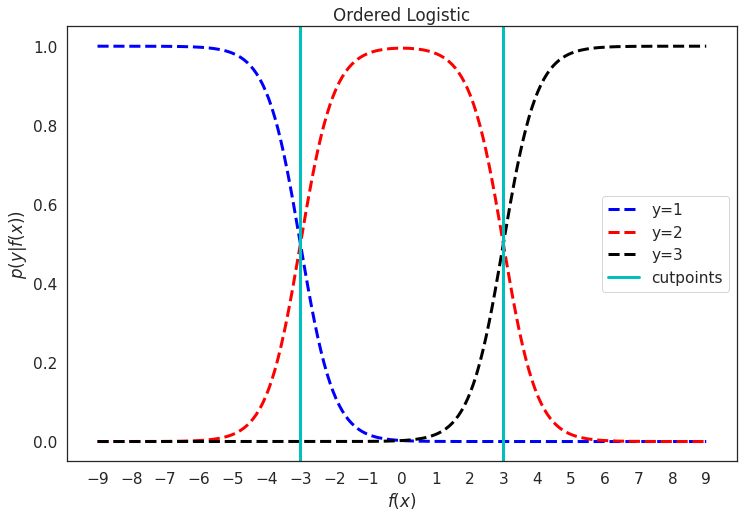
\includegraphics[width=0.8\textwidth]{content/chapters/semi_supervised_pchmm_missing_data/images/ordered_logistic.png}
}
\caption{Visualization of likelihood function for ordinal regression with 3 classes using the logistic distribution to simulate latent function noise}
\label{fig:clm_likelihood_vs_g}
\end{center}
\end{figure}

\textbf{Semi-supervised learning of HMMs via prediction-constrained training}

Now that our generative and discriminative model components are defined, we wish to \emph{estimate the parameters} of the model from a labeled training set $\mathcal{D}^L$ and an (optional) unlabeled set $\mathcal{D}^U$.

The first approach, simple and commonly used~\citep{sotoodeh2019improving}, is two-phase training that first fits standard HMM parameters $\pi, \mu, \sigma$ to all feature data (labeled and unlabeled), then fits the prediction parameters $\eta, \theta$ on the labeled set only.
\begin{align}
\text{phase 1:}~~
\hat{\pi}, \hat{\mu}, \hat{\sigma} &\gets \arg\max_{\pi, \mu, \sigma} \sum_{\xobs \in \mathcal{D}^L \cup \mathcal{D}^U} \log p( \xobs | \pi, \mu, \sigma ),
\label{eq:objective_two_stage}
\\ \notag 
\text{phase 2:}~~~~~
\hat{\eta}, \hat{\theta} &\gets \arg \max_{\eta, \theta} \sum_{\xobs, y ~\in \mathcal{D}^L} \log p( y | \xobs, \eta, \theta, \hat{\pi}, \hat{\mu}, \hat{\sigma}).
\end{align}
In phase 2, prediction parameters are estimated to maximize the label-given-feature likelihood, which is Eq.~\eqref{eq:binary_classification} for binary classification (where $\theta$ is unneeded) or Eq.~\eqref{eq:ordinal_lik} for ordinal regression.
Both objectives can be computed via HMM dynamic programming routines and are amenable to modern automatic differentiation, enabling estimating solutions via gradient descent algorithms.
For such algorithms, constrained parameters such as initial state probabilities \(\pi_0\), state transition probabilities \(\pi_k\), and Gaussian emission variances \(\sigma\) are reparameterized into the unconstrained real space so that all gradient updates yield valid parameters.
Phase 1 can also be solved with expectation-maximization~\citep{ghahramaniIntroductionHiddenMarkov2001b}.

The potential downside to the above approach is that the HMM is trained in an \emph{unsupervised} fashion. Class labels $y$ do not inform the values of $\pi, \mu, \sigma$.
Alternatively, we can maximize the joint supervised likelihood of features and any available labels: 
\begin{align}
    \pi, \mu, \sigma, \eta, \theta \gets
        \arg \max \sum_{\xobs, y \in \mathcal{D}^L}
            \log p( \xobs, y | \eta, \theta, \pi, \mu, \sigma) 
    + \sum_{\xobs \in \mathcal{D}^U}
    \log p( \xobs | \pi, \mu, \sigma)
\label{eq:objective_supervised_joint}
\end{align}
Again, both terms (and their gradients) can be computed in straightforward fashion, as in the two-stage method above.
The main issue with this approach is that while labels can inform the values of the HMM parameters $\pi, \mu, \sigma$, the objective does not encode our practical goal to prioritize predicting labels from features well even when we have few labels. 
This deficiency is reflected in our later results in Figure \ref{fig:mortality_prediction_results}, where this ``supervised'' approach to HMM training is hardly better than the two-stage unsupervised-then-predict method when we have few labels ($N \ll M$).

Recognizing the limitations of these methods, we arrive at our proposed \emph{prediction-constrained} (PC) objective, which directly encodes our goals: first and foremost, achieve label-from-feature prediction better than some threshold $\epsilon$, while also learning a good generative model if possible (to improve handling of missingness). Formally, we wish to estimate parameters by solving the constrained objective

\begin{align}
\pi, \mu, \sigma, \eta, \theta \gets \arg\max & \sum_{\xobs \in D^L \cup D^U} \log p(\xobs | \pi, \mu, \sigma) 
\label{eq:standard_pc_constrained},
\\ \notag
\text{subj. to:} \quad & 
\sum_{\xobs, y \in D^L} \log p(y | \xobs, \pi, \mu, \sigma, \eta, \theta) \geq \epsilon.
\end{align}

Directly handing the constraint here is difficult, so we transform the problem to be more amenable to modern gradient-based learning. 
By applying the theory of Langrange multipliers~\citep{bertsekasConstrainedOptLagrange1996}, we can form an equivalent unconstrained PC objective
\begin{align}
\pi, \mu, \sigma, \eta, \theta \gets \arg\max \sum_{\xobs \in D^L \cup D^U} \log p(\xobs | \pi, \mu, \sigma) 
+ ~~\lambda \sum_{\xobs, y \in D^L} \log p(y | \xobs, \pi, \mu, \sigma, \eta, \theta).
\label{eq:standard_pc_unconstrained}
\end{align}
For each tolerance $\epsilon$, there exists a scalar $\lambda > 0$  such that the maximizer of Eq.~\eqref{eq:standard_pc_unconstrained} 
is an optimum of Eq.~\eqref{eq:standard_pc_constrained}. 
Scalar $\lambda$ thus plays an analogous role as $\epsilon$ in the constrained objective; to achieve a higher prediction quality $\epsilon$, we would solve the above with a larger $\lambda$. 
In the special case of $\lambda = 1$, we recover the earlier supervised objective in Eq.~\eqref{eq:objective_supervised_joint}. 
We intend usually that $\lambda \gg 1$, which encourages better predictions of $y$ from $x$, trading off the quality of generative modeling of $x$ when necessary.


% \textbf{Prediction constrained training.} 
% Now that our generative and discriminative components are defined, we show how the prediction constrained framework is adapted to semi-supervised learning.
% We wish to fit the parameters of the HMM to a labeled dataset $\mathcal{D}^L$ containing many pairs of feature time-series $X$ and class label $y$ as well as an optional unlabeled dataset $\mathcal{D}^U$ containing only $X$ for many sequences.
% Prediction constrained training~\citep{hopePredictionConstrainedHiddenMarkov2021} aims to maximize generative performance but is unwilling to sacrifice prediction quality (the two aims are not treated equally).
% %seek an optimal fit for generating the time-series data (using the HMMs emission distribution($\phi$) to generate observations $x_n$ given a latent state, and the transition distribution($\pi$) to capture state transition at consecutive time-points), and simultaneously predict the labels $y_n$ (using beliefs from the HMM) accurately. 
% Our PC objective to minimize is
% \begin{align}
% %\resizebox{.6\hsize}{!}{$
% \mathcal{L}(\pi, \phi, \eta)
% \triangleq
% \sum_{X \in \mathcal{D}^L \cup \mathcal{D}^U}{{-}\log p( X^{\mathcal{O}} | \pi, \phi)}
% - \lambda 
% \sum_{X,y \in \mathcal{D}^L}{\log p(y|X, \pi, \phi, \eta)}
% %$}
% \end{align}

% The predictor distribution $p(y|X, \pi, \phi, \eta)$ is replaced by equation \ref{eq:binary_classification} or equation \ref{eq:ordinal_lik} for binary classification or ordinal regression respectively. To emphasize the classification task's importance, we set tradeoff parameter $\lambda \gg 1$, selecting its specific value via a validation set.

\textbf{PC-HMM Initialization}: We initialize the HMM's emission's parameters using K-means clustering. For ordinal regression, we initialize the emission's parameters for each class separately and then aggregate the learned clusters by retaining the states that are maximally distant from each other. We set the HMM's initial state probabilities to a uniform with probability $1/K$. For the transition distribution, we initialize such that self transitions probabilities (diagonal elements of the transition matrix) are 0.5, while the off-diagonal entries are $0.5/(K-1)$.We initialize the predictor weights by training a supervised model (logistic regression for binary classification or ordered logistic for ordinal regression) using the initial beliefs as features. We additionally apply L2 regularization on the predictor weights to prevent overfitting.


\subsection{Justifying Usage of The Prediction Constrained (PC) Framework}
The PC framework is built to model tasks containing both labelled and unlabelled examples. In case of time-series health record datasets, unlabelled examples include medical records (including vitals, lab measurements, medications etc.) of patient stays for whom outcome labels may not be available (for example, due to the high cost of obtaining clinician annotated disease labels). In contrast, labelled examples include medical records of patient stays for whom clinician annotated labels exist. The goal of the PC framework is to improve the predictive performance on labelled examples (over a fully supervised approach) by utilizing the unlabelled examples. This is done by maximizing the generative performance on both the labelled and unlabelled examples. While simultaneously adhering to performance constraints on the labelled set.

To formulate the core principle of the PC framework and highlight it's benefits, we first consider a more generic training approach,  \textit{regularized joint maximum likelihood optimization}. We consider a dataset $D$ containing labelled examples $D^L=\{x_n, y_n\}_{n=1:N^{L}}$ and unlabelled examples $D^{U}=\{x_n\}_{n=1:N^{U}}$. Additionally, we assume $h_n$ is a hidden variable, such that the generative process is as follows : (1) Generate $h_n$ from prior distribution parameterized by $\xi^h$; (2) Generate $x_n$ given $h_n$ from a distribution parameterized by $\xi^x$; (3) Generate $y_n$ given $x_n$ and $h_n$ parameterized by $\xi^y$. The joint distribution over $x_n, y_n, h_n$ is as follows :

\begin{align}
    p(x_n, y_n, h_n|\xi^h, \xi^x, \xi^y)=p(h_n|\xi^h)p(x_n|h_n, \xi^x)p(y_n|x_n, h_n, \xi^y)
\end{align}

Regularized maximum likelihood minimizes the following objective and obtains the optimal parameters $\xi^{ML}$.

\begin{align}
    \xi^{ML} = \min_{\xi=\{\xi^h, \xi^x, \xi^y\}} -\Sigma_n \log p(x_n, y_n|\xi) + R(\xi)
\end{align}
where $R(\xi)$ is the regularizer on the model parameters. 
The main issue with regularized maximum likelihood is that it assumes a symmetric relationship between $x_n$ and $y_n$. In other words, jointly maximizing the likelihood of $x_n$ and $y_n$ does not clearly highlight the practitioner's goal of predicting $y_n$ given $x_n$, rather than $x_n$ given $y_n$. To overcome this issue, the PC framework clearly specifies the need to learn a generative model for data $x$ that simultaneously achieves some threshold performance $\epsilon$ while predicting $y$ from $x$ with the following objective.
\begin{align}
\min_{\xi=\{\xi^h, \xi^x, \xi^y\}} \quad & -\Sigma_{n\in D^L \cup D^U} \log p(x_n|\xi^h, \xi^x) + R(\xi),
% \label{eq:standard_pc_constrained}
\\ \notag
\text{subj. to:} \quad & 
-\Sigma_{n\in D^L} \log p(y_n|\xi^h, \xi^x, \xi^y)\leq \epsilon
\end{align}

By applying the theory of Langrange multipliers, the unconstrained PC objective is :
\begin{align}
    \xi^{PC}=\min_{\xi=\{\xi^h, \xi^x, \xi^y\}} -\Sigma_{n\in D^L \cup D^U} \log p(x_n|\xi^h, \xi^x) - \lambda \Sigma_{n\in D^L} \log p(y_n|\xi^h, \xi^x, \xi^y) + R(\xi)
% \label{eq:standard_pc_unconstrained}
\end{align}
The PC objective clearly prioritizes predictions of $y_n$ from $x_n$ by setting $\lambda>1$ and eliminates the symmetric assumption between $x_n$ and $y_n$. 
This is also justified empirically in Figures \ref{fig:mortality_prediction_results} and \ref{fig:MIMIC_los_prediction_results}, where we see that models trained with the PC objective ($\lambda>>1$) always outperform models trained with maximum likelihood ($\lambda=1$, shown as supervised HMM), and models where the supervised and unsupervised components are trained separately in a 2 step process ($\lambda=0$, shown as unsupervised HMM $+$ predictor). In the following sub-sections, we show how the PC framework is applied to time-series data by choosing a HMM as the generative component. We further show how missing data can be handled elegantly without the need for imputation, and how missing labels can be handled via the semi-supervised extension of the PC framework for clinical prediction tasks involving binary classification as well as ordinal regression.

% \subsection{Baseline Semi-supervised learning adapted to Time-Series}

% Recent progress in improving deep classifiers in the SSL setting has been made under the family of \emph{consistency regularization}.
% Following the unified analysis in \citet{zhuRichGetRicher2022}, these approaches train a deep network $f_{\theta}$ with weights $\theta$ to minimize a two-term loss:

% \begin{align}
% \sum_{X, y \in \mathcal{D}^L }{\ell( y, f_{\theta}(X) )}
%  + \lambda \hspace{-6pt}
%  \sum_{X \in \mathcal{D}^U}{\ell( y'(X), f_{\theta}(X) )}
% \end{align}
% Here, $\ell(\cdot, \cdot)$ is a loss function, $\lambda > 0$ is a tradeoff hyperparameter, $y'(X)$ is a labeling transformation, and $a(\cdot)$ represents an (optional) data augmentation transformation.
% Below, we describe how both MixMatch and FixMatch fit this framework via concrete realizations of $y'$, $a$, and $\ell$.

% In practice, to minimize this loss via minibatch gradient descent we start $\lambda$ at zero for a few hundred epochs, and gradually ramp up to a small positive value over a few hundred more epochs.
% This ensures that early learning fits well to the labeled set, while letting the unlabeled set also influence results later on.

% \textbf{MixMatch for time series.}
% MixMatch~\citep{berthelotMixMatchHolisticApproach2019} is a recent state-of-the-art SSL algorithm based on two key ideas.
% First, smooth transitions between classes in feature space are desirable and achievable via an interpolating augmentation scheme known as MixUp~\citep{zhangMixupEmpiricalRisk2017}.
% Second, it is useful to ensure consistency in the predicted label across multiple augmentations of the same source features.
% Originally designed for images, it has recently been applied to time series  \citep{goschenhofer2021deep}.
% % to encourage smooth transitions between classes and encourages all augmentations of the same source features to lead to the same predictions.

% We set the labeling function $y'(X)$ to produce temperature-sharpened probability vectors averaged across multiple augmentations of examples X.
% The augmentation transformation $a(\cdot)$ uses MixUp to interpolate between labeled examples (see \citep{berthelotMixMatchHolisticApproach2019} for details).
% As a basic augmentation procedure applicable to time series, we add Gaussian noise $\mathcal{N}(0, \epsilon^2)$, following \citet{goschenhofer2021deep}, with standard deviation $\epsilon$ set to 0.1 and 1.
% For the backbone architecture $f_{\theta}$, we use a Gated Recurrent Unit(GRU)~\citep{gru_original}.

% \textbf{FixMatch for time series.}
% Similar to MixMatch, FixMatch~\citep{sohnFixMatchSimplifyingSemisupervised2020} is another recent state-of-the-art SSL algorithm based on consistency regularization and pseudo-labeling. Pseudo-labels for weakly augmented unlabeled examples are only retained if the model produces high-confidence predictions (we try 0.6 and 0.8 as thresholds for high confidence predictions). Consistency regularization and the augmentation procedure is the same as MixMatch. Again, we use GRU for the backbone architecture.

% \subsection{Baselines for Supervised Learning With Time-Series}
% \textbf{Gated Recurrent Unit with Decay (GRU-D)} GRU-D \citep{cheRecurrentNeuralNetworks2018} The GRU-D model is an adaptation of the standard GRU (Gated Recurrent Unit) architecture, tailored specifically for handling clinical time series data with missing values and irregular time intervals. GRU-D elegantly addresses the challenges of modeling clinical data by integrating information about missingness patterns and elapsed time between observations directly into the model.

% GRU-D extends the GRU by incorporating two main components: decay mechanisms for missing values and modeling elapsed time between observations.
% \begin{itemize}
%     \item Masking : GRU-D uses a masking mechanism to handle missing values. For each input feature, a binary mask (denoted as $m$ is used, which has a value of 1 if the feature is observed and 0 if it's missing. This mask is used to modulate the input and decay rates.
%     \item Decay Rate: This is a mechanism in GRU-D to capture the elapsed time between two consecutive observations. This decay rate ensures that the effect of a distant past observation decreases as time progresses.
% \end{itemize}

% The equations for GRU-D with the missing data handling and decay mechanisms can be described as:
% \begin{align*}
%     &\gamma_t = \text{tanh}(W_d \delta_t + b_d)\\
%     &h'_{t-1} = m_t \odot h_{t-1} + (1 - m_t) \odot (\gamma_t \odot h_{t-1})
% \end{align*}
% Where $\gamma_t$ is the decay rate, $\delta_t$ is the elapsed time since the last observation and $h'_{t-1}$ is the decayed previous hidden state.
% The decayed hidden state $h'_{t-1}$ replaces the regular $h_{t-1}$ in the GRU equations. $W_d$ and $b_d$ are learned parameters and $m_t$ represents the missingness mask (1 means observed, 0 means missing)

% The last hidden state is then passed through the fully connected layers to get the final classification output:
% \begin{align*}
%     \hat{y} = f_{out}(W_c h_T + b_c)
% \end{align*}
% Where $W_c$  and $b_c$ are trainable parameters of the fully connected layer. $h_T$ is the final hidden state from GRU-D.
% $f_{out}$ is the fully connected output layer.

% This output $\hat{y}$ is then used to compute the classification loss, using binary cross-entropy, which is then minimized during training.

% \textbf{Bidirectional Recurrent Imputation Time Series (BRITS)} BRITS \citep{caoBRITSBidirectionalRecurrent2018} is designed as a bidirectional RNN that performs imputation and classification/regression jointly in one neural graph. The hidden states are computed in both directions and concatenated to capture context from past and future time steps:
% \begin{align*}
%     &\overrightarrow{h}_t = \text{RNN}\left(\overrightarrow{h}_{t-1}, x_t\right) \tag{Forward RNN}\\
%     &\overleftarrow{h}_t = \text{RNN}\left(\overleftarrow{h}_{t+1}, x_t\right)
%     \tag{Backward RNN}\\
%     & h_t = [\overrightarrow{h}_t, \overleftarrow{h}_t]
%     \tag{combined hidden state}
% \end{align*}
% Finally, the sequence label $\hat{y}$ is predicted as 
% \[
% \hat{y} = f_{out}(\Sigma_{i=1}^T\alpha_i h_i)
% \]
% where $f_{out}$ is the output layer and $\alpha_i=1/T$.
% If a measurement $x_t$ at time $t$ is missing, it is replaced by a complement value $\hat{x_t}=W_x h_{t-1}+b_x$ where $W_x$ and $b_x$ are learned parameters. Additionally, the model incorporates a consistency loss to enforce the prediction in each step to be consistent in both directions. The consistency loss at time $t$ is given by $l_t^{cons}(\hat{x_t}, \hat{x_t'})=MAE(\hat{x_t}, \hat{x_t'})$, where $x_t$ is the estimated sequence in the forward direction and $\hat{x_t'}$ is the estimated sequence in the backward direction. The final loss $l$ is given by
% \begin{align*}
%     l = \Sigma_{t=1}^T l_t^{cons}(\hat{x_t}, \hat{x_t'}) + l_t^{imp}(x_t, \hat{x_t})+l^{BCE}(y, \hat{y})
% \end{align*}
% where $l_t^{cons}$ is the mean absolute error applied to the missing observations, $l_t^{imp}$ is the mean absolute error applied to the observed dimensions and $l^{BCE}$ is the binary cross entropy for classifying the output.

\subsection{Baseline neural nets for fully-supervised classification with missingness}
\label{sec:baselines_RNN}

We now consider alternative deep models intended to produce effective predictions for clinical time series, even with some missingness, but that can only make use of labeled datasets. These approaches cannot easily benefit from an extra large unlabeled dataset $\mathcal{D}^U$. We focus specifically on two methods in the recurrent neural net tradition that are both well-known and competitive: the Gated Recurrent Unit with Decay (GRU-D)~\citep{cheRecurrentNeuralNetworks2018} and Bidirectional Recurrent Imputation Time Series (BRITS)~\citep{caoBRITSBidirectionalRecurrent2018}, each summarized below.

\textbf{GRU-D : Gated recurrent Unit with decay model} \citep{cheRecurrentNeuralNetworks2018} developed the GRU-D to adapt the standard GRU (Gated Recurrent Unit) architecture by~\citep{gru_original} in order to specifically handle clinical time series data with missing values and long time delays between non-missing values. 
GRU-D extends the GRU by producing a complete feature vector at every time step, imputing any missing values between the last observation and a population mean via a  learnable, variable-specific decay mechanism informed by the time since last observation. Another similar decay mechanism informs the GRU-D's continuous-valued hidden state vector.
Ultimately, like any recurrent neural net, the GRU-D can be viewed as a deterministic mapping of input time series $\mathbf{X}$ of length $T$ to a representation vector $h_T$ at the final timestep. Following \citep{cheRecurrentNeuralNetworks2018}, a fully-connected output layer maps $h_T$ to probabilities over the $C$ possible classes. 

\textbf{BRITS : Bidirectional Recurrent Imputation Time Series model} \citep{caoBRITSBidirectionalRecurrent2018} designed BRITS as a bidirectional RNN that jointly performs imputation and classification/regression. It generates forward and backward hidden state representations, concatenates them into per-timestep representations $h_t$, and creates a sequence-level representation through mean pooling, followed by a fully-connected layer to produce class probabilities. The BRITS model handles missing data by using bidirectional recurrent neural networks that incorporate both past and future information, leveraging temporal correlations to impute missing values while considering the entire sequences, but its reliance on future data makes it unsuitable for real-time applications.

In our implementation, for both GRU-D and BRITS weight parameters are trained via gradient descent exclusively on the labeled training set $\mathcal{D}^L$ to minimize cross entropy. BRITS also includes a reconstruction and imputation consistency loss. For both methods, key hyperparameters like network size and learning rate settings are tuned on the validation set of each task. See table \ref{table: hyperparameters} for details.


\subsection{Baseline neural nets for semi-supervised time series classification without missingness}
\label{sec:baselines_SSL}

Many works have aimed to develop deep classifiers for SSL scenarios without abundant labeled data but plenty of unlabeled data. In this work, we focus on two strong baselines from the deep SSL literature, MixMatch~\citep{berthelotMixMatchHolisticApproach2019} and FixMatch~\citep{sohnFixMatchSimplifyingSemisupervised2020}. MixMatch recently delivered the most reliable accuracy gains (even over more recent methods) at a benchmark of self-supervised and semi-supervised methods for medical images \citep{huang2023accuracy}.
%of the SSL setting has been made under the family of \emph{consistency regularization}.
We adapt both methods to time series following \citep{goschenhofer2021deep}.
Importantly, neither method natively handles time series with arbitrary missingness. Thus, all methods here assume missing values have been filled by forward filling imputation (for all times after the first observation of channel $d$) or mean imputation (for all other times).
%fills in any missing values of any feature time series in any dataset.

Following the unified analysis of many SSL methods in \citep{zhuRichGetRicher2022}, these approaches train a deep network $f_{w}$ with weights $w$ to minimize a two-term loss:
\begin{align}
w^* \gets \arg\min \compactsum{X, y \in a(\mathcal{D}^L) }{\ell( y, f_{w}(X) )}
 + \lambda \hspace{-6pt}
 \compactsum{X \in a(\mathcal{D}^U)}{\ell^U( y'(X), f_{w}(X) )}
\end{align}
Here, $\ell(\cdot, \cdot)$ is a standard classification loss (e.g. binary cross entropy) and $\ell^U$ a corresponding unlabeled set loss, $\lambda > 0$ is a tradeoff hyperparameter, $y'(X)$ is a labeling transformation, and $a(\cdot)$ represents an (optional) data augmentation transformation. Below, we describe how both MixMatch and FixMatch fit this framework via distinct realizations of augmentations $a$ and loss $\ell^U$. 

Our implementation of both MixMatch and FixMatch uses a Gated Recurrent Unit (GRU)~\citep{gru_original} architecture to obtain a vector representation for the entire time series. 
We make predictions using representations from the last time step of each sequence.
For both methods, weights \( w \) are estimated using minibatch gradient descent with the Adam \citep{kingma2014adam} optimizer, starting with the unlabeled loss weight \( \lambda \) at zero and gradually increasing it \citep{tarvainen2017mean, berthelot2019mixmatch}. Key shared hyperparameters like \( \lambda \), GRU network size, and learning rate, as well as method-specific hyperparameters, are tuned on the validation set.

\textbf{MixMatch for time series.}
MixMatch is a semi-supervised learning algorithm that improves model performance by combining data augmentation, pseudo labels produced by the classifier, and a consistency loss to effectively utilize both labeled and unlabeled data. To adapt MixMatch \citep{berthelotMixMatchHolisticApproach2019} to time series, we follow Goschenhofer et al. \citep{goschenhofer2021deep}. For each input time series, we have all missing values imputed and then apply z-score transformations to standardize features.
Next, we apply two kinds of augmentation: add Gaussian noise \(\mathcal{N}(0, \epsilon^2)\) and apply MixUp \citep{zhangMixupEmpiricalRisk2017}, which interpolates between random pairs of features $\mathbf{X}$ and their labels (or pseudo labels) to create synthetic examples. We sample each pair's interpolation ratio from the distribution \(\text{Beta}(\alpha, \alpha)\). 
MixMatch defines loss $\ell^U$ to enforce label consistency between the model's prediction on an unlabeled instance and the average temperature-sharpened probability vector from several augmentations of that instance.
The key hyperparameters for MixMatch are scalars $\epsilon$ and $\alpha$. 



\textbf{FixMatch for time series.}
FixMatch \citep{sohnFixMatchSimplifyingSemisupervised2020} combines weak and strong augmentations to create diverse versions of unlabeled data, enabling the model to learn robust features by consistently predicting the same labels across these variations. Weak augmentations provide stable pseudo-labels, while strong augmentations introduce robustness by challenging the model with heavily altered data. To adapt FixMatch to time series, we add random Gaussian noise sampled from \(\mathcal{N}(0, 0.01)\) for weak augmentations and from \(\mathcal{N}(0, 1)\) for strong augmentations. Unlike \citep{goschenhofer2021deep}, who use RandAugment \citep{cubuk2020randaugment}, we only add Gaussian noise since time and magnitude warping hurt performance in our experiments. Pseudo-labels for weakly augmented examples are retained if the model produces high-confidence predictions, with thresholds of 0.6 and 0.8 explored. FixMatch's unlabeled loss $\ell^U$ uses these pseudo-labels as targets for strongly augmented versions of the same examples, ensuring consistent predictions across augmentations and leveraging high-confidence predictions to enhance model robustness and generalization.


\subsection{Justification of the $O(TK^2)$ belief computation runtime for HMMs}

The complexity largely stems from the number of states and the transitions between these states considered over the length of the observation sequence in an algorithm termed as Forward Backward Algorithm.

The forward algorithm computes the probability of observing the sequence up to time \( t \) and being in state \( k \). This is known as the forward probability, denoted as \( \alpha_t(k) \). The recursion formula for \( \alpha_t(k) \) is given by:

\[
\alpha_t(k) = \left( \sum_{j=1}^K \alpha_{t-1}(j) a_{jk} \right) b_k(o_t)
\]

Where:
\begin{itemize}
    \item \( \alpha_{t-1}(j) \) is the forward probability of being in state \( j \) at time \( t-1 \).
    \item \( a_{jk} \) is the transition probability from state \( j \) to state \( k \).
    \item \( b_k(o_t) \) is the probability of observing \( o_t \) given state \( k \) (the emission probability).
\end{itemize}


Computational Steps:
\begin{itemize}
    \item For each state \( k \) at each time \( t \), calculate \( \alpha_t(k) \).
    \item For each \( k \), the sum is over all \( K \) possible states \( j \), requiring \( K \) multiplications and \( K-1 \) additions.
    \item Thus, for each \( k \) and each \( t \), the computation is \( O(K) \).
    \item Since there are \( K \) states to consider at each time step, the complexity for each \( t \) is \( O(K^2) \).
\end{itemize}


Similarly, the backward algorithm computes the probability of the future observations given state \( k \) at time \( t \). This is known as the backward probability, denoted as \( \beta_t(k) \). The recursion formula for \( \beta_t(k) \) is given by:

\[
\beta_t(k) = \sum_{j=1}^K a_{kj} b_j(o_{t+1}) \beta_{t+1}(j)
\]

Where:
\begin{itemize}
    \item \( \beta_{t+1}(j) \) is the backward probability at state \( j \) at time \( t+1 \).
    \item \( a_{kj} \) is the transition probability from state \( k \) to state \( j \).
    \item \( b_j(o_{t+1}) \) is the emission probability at state \( j \) for observation \( o_{t+1} \).
\end{itemize}

Since both the forward and backward algorithms require \( O(K^2) \) operations at each of the \( T \) time steps, the overall computational complexity for running either algorithm is \( O(TK^2) \). This describes the amount of computational work needed to process an entire sequence with respect to the number of states and the length of the sequence, making clear the impact of the state space size and the sequence length on the computational demand.
\section{Results}
\subsection{Toy Data Experiment}
\label{app_toy_data_gen}
The 2-D toy data (represented as $x=\{x_1, x_2\}$) is generated from a Markov model with 4 states (states 0, 1, 2, 3) with the means of the emission distributions located at $(0, -1), (8, -1), (13, 0)$ and $(24, 0)$. The variance in $x_1$ is 0.3 and variance in $x_2$ is 1 for each of the clusters. Each sequence is initialized at state 0 and either remains in the current state or transitions to the next adjacent state with equal probability. Once state 2 is reached, it immediately transitions to state 3 in the next time-step and stays there for the remaining time-steps with probability 1. We simulate 350 sequences, each of length $T=8$ from this model. A sequence is labeled as 1 if it enters the highlighted black box highlighted in figure \ref{fig:toy_pchmm} at any time-point. At each time-point and dimension, data is missing with a fixed probability ($\rho$). We vary $\rho$ on the right plot of figure \ref{fig:toy_pchmm} and report classification performance against several baselines. 

\textbf{Findings :}
We analyze a toy dataset of many sequences generated by an HMM with $K=4$ Gaussian clusters in a $D=2$ feature space. The 2D features are illustrated in Fig.~\ref{fig:toy_pchmm}:
Each sequence is labeled $y=1$ only if any timestep's feature $x_t$ enters the black square.
Fig.~\ref{fig:toy_pchmm} (left) shows that even at 40\% missingness (i.i.d. across features and timesteps) the PC-HMM with $K=6$ learns separate states that cover the black box and its complement, and thus are \emph{discriminative}.
In contrast, both mean-filling and forward-filling imputation destroy the separability of red and blue classes. 
In Fig.~\ref{fig:toy_pchmm} (right), at all missingness levels the PCHMM delivers better AUROC than alternatives, including an LSTM and the GRU-D. This dataset is class-balanced, thus AUROC is an appropriate metric. Later mortality prediction tasks are imbalanced, so we use area under the precision recall curve (AUPRC) instead.
All PC-HMM results, including ``with mean-filled/forward-filled'' baselines, assume diagonal covariances.

\setlength{\tabcolsep}{.1cm}
\begin{figure*}[!t]
\begin{tabular}{c c}
    \centering
% Suggestion 1: Always specify either height or weight
% Suggestion 2: Make sure the aspect ratio when exported matches the intended ratio in the paper here
    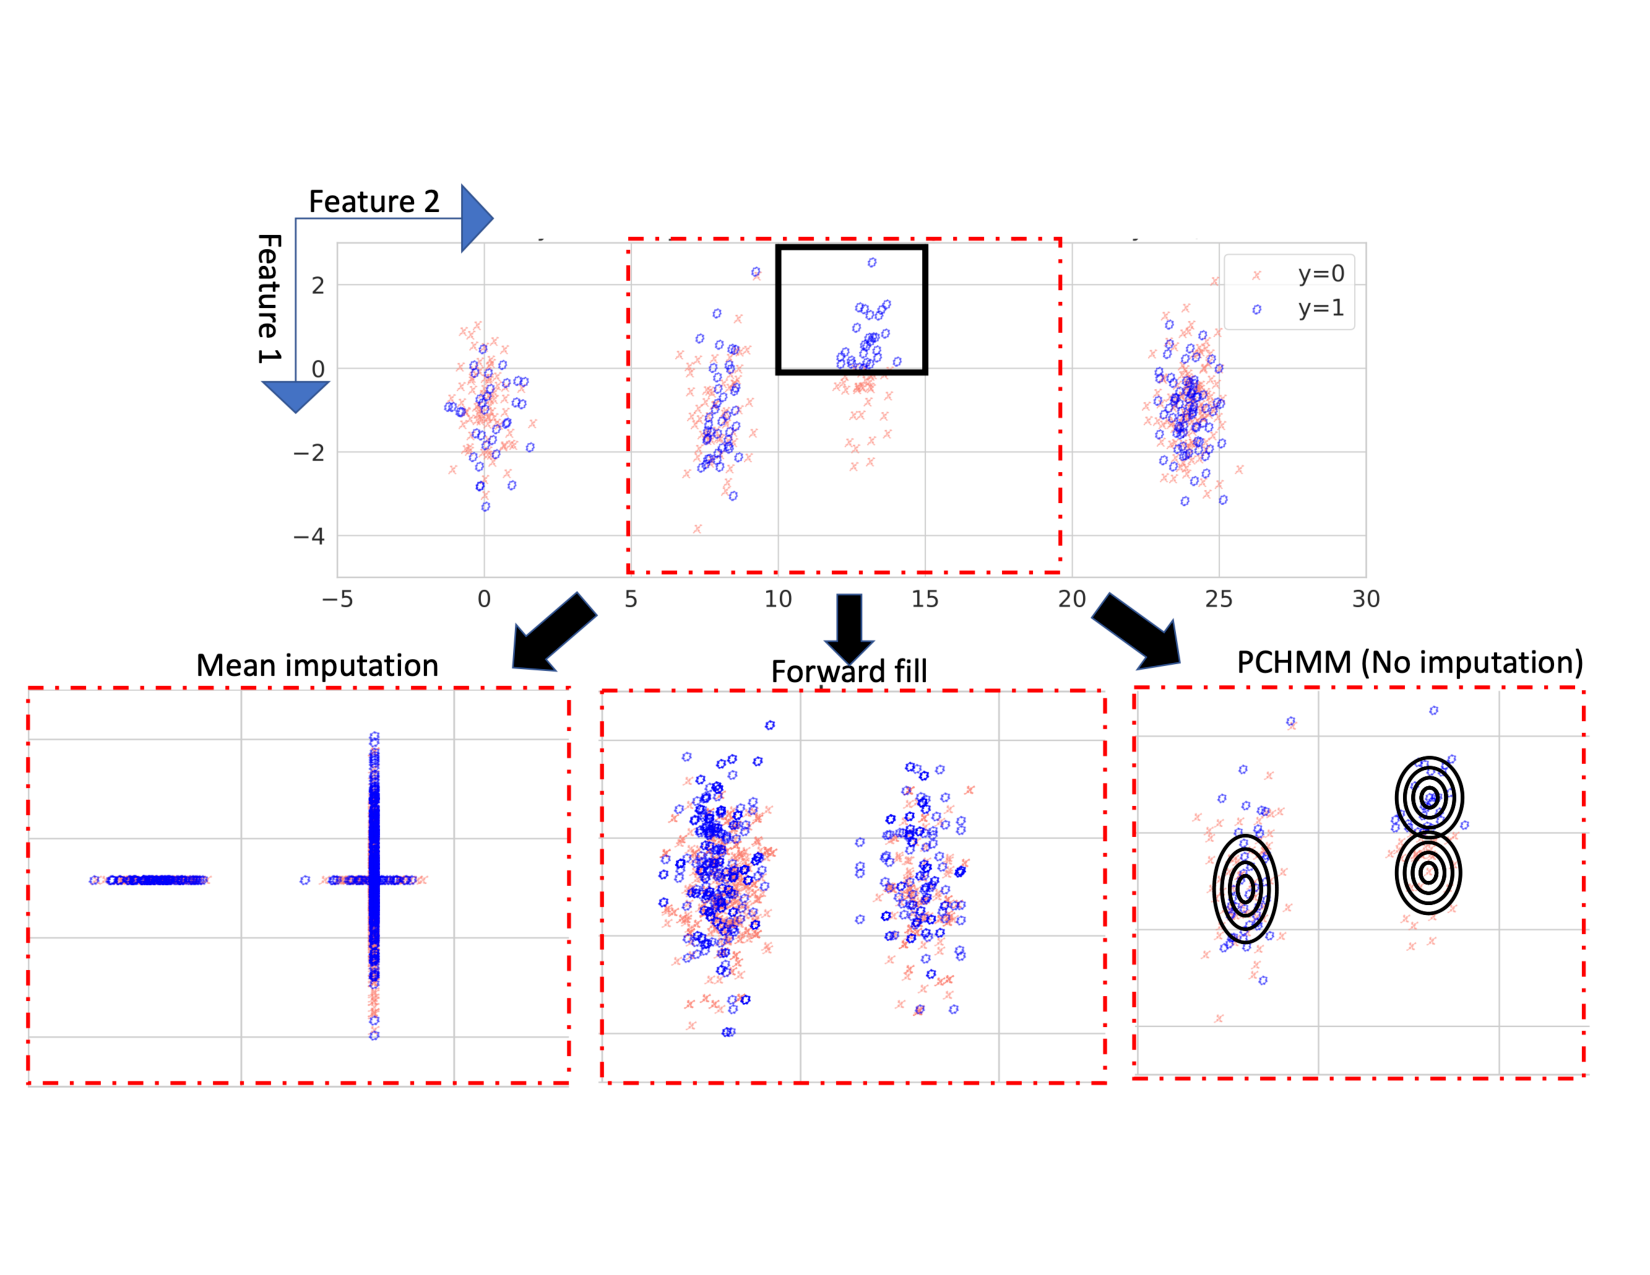
\includegraphics[width=0.57\textwidth]{content/chapters/semi_supervised_pchmm_missing_data/images/toy_data_fig.pdf}
    &
    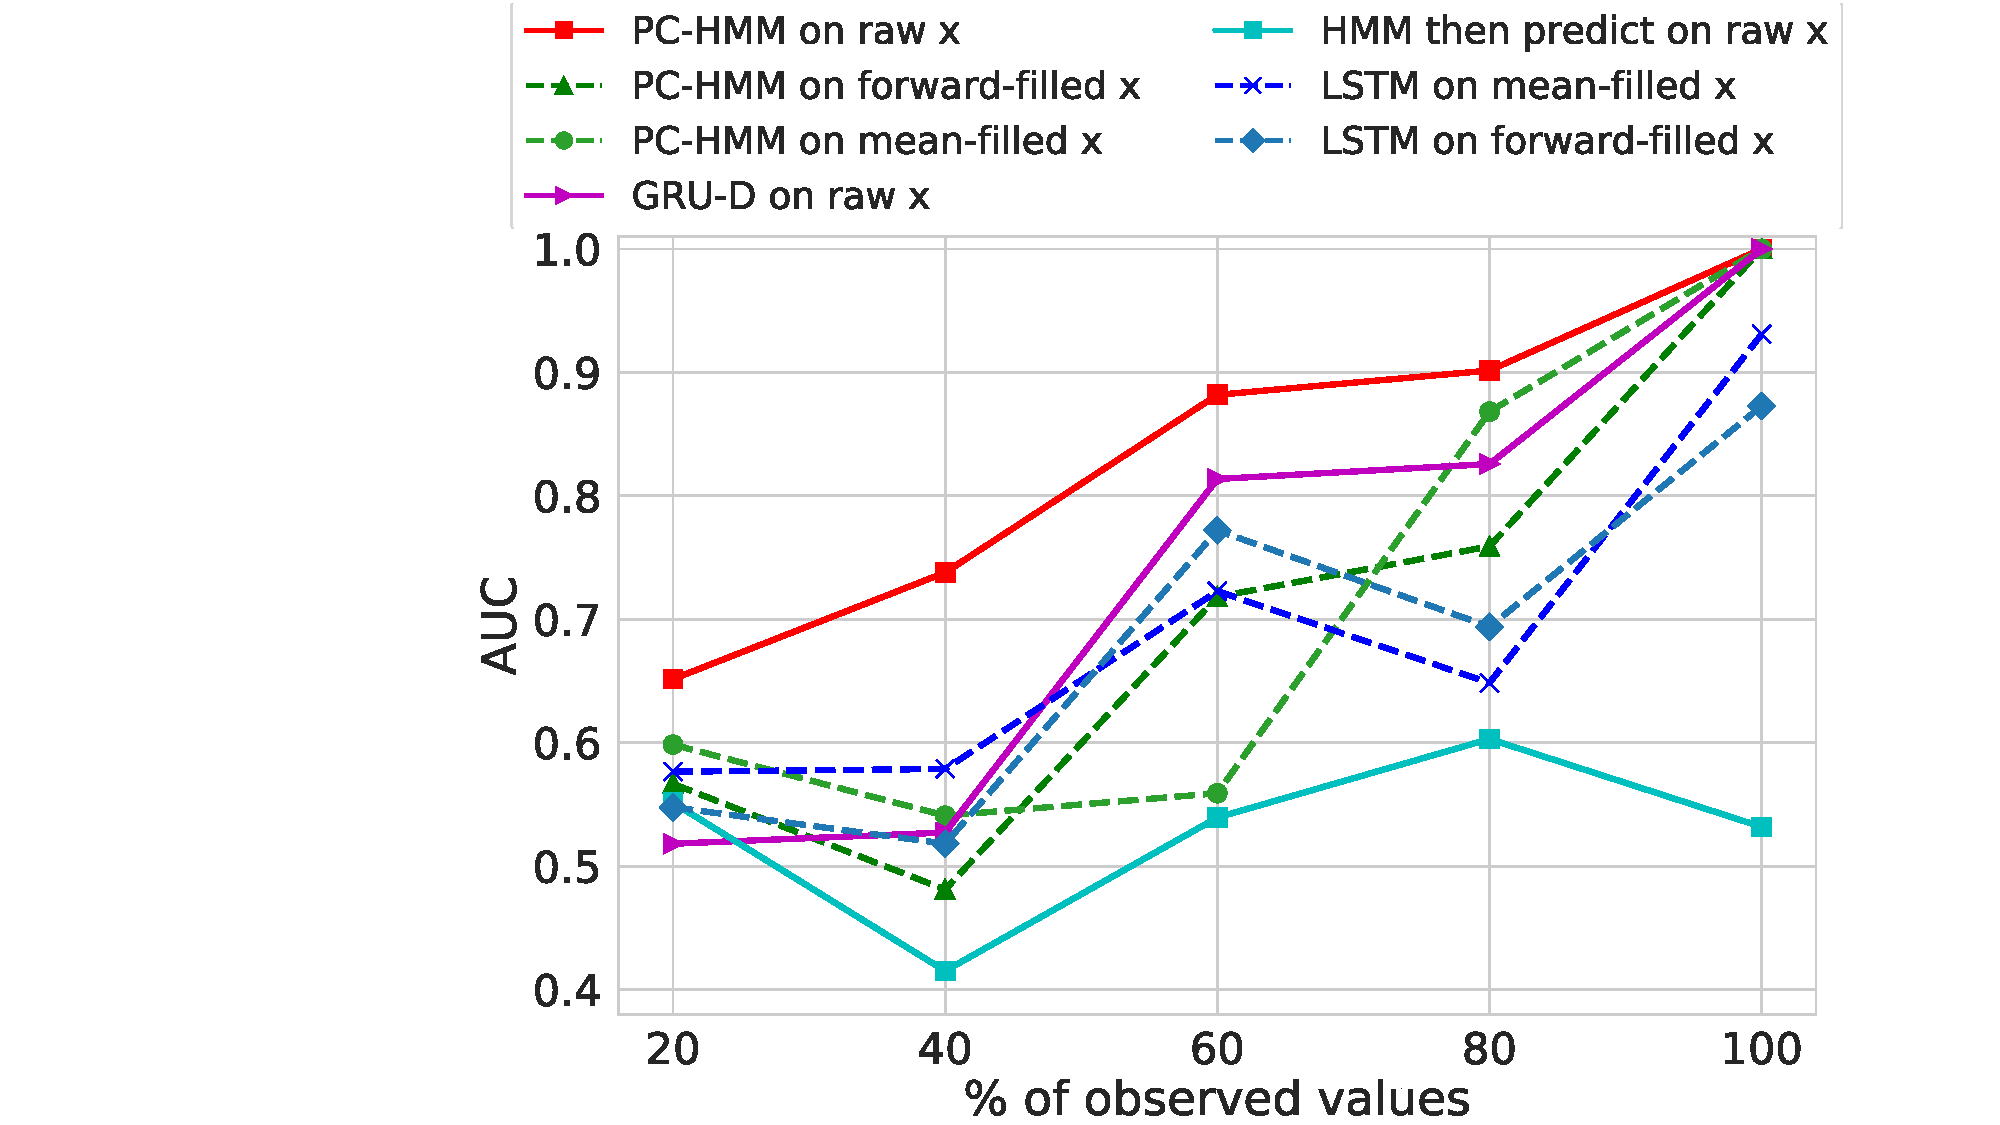
\includegraphics[width=0.43\textwidth]{content/chapters/semi_supervised_pchmm_missing_data/images/toy_data_perf_fig.pdf}
\end{tabular}
\caption[Demonstration of proposed PC-HMM on an “easy” binary classifier
task where naive imputation fails]{Demonstration of proposed PC-HMM on an ``easy'' binary classifier task where naive imputation fails.
\textbf{\emph{Top left:}} Visualization of all observed 2D features from 350 sequences (x-axis: feature 1 value, y-axis: feature 2), colored by labels and collapsed over time.
Each sequence ($T{=}8$) comes from a Markov model that generates features from the 4 clusters shown in this 2D feature space.
A sequence's class label depends on if \emph{any observation} lands in the black box (yes means $y=1$, no means $y=0$). 
Without missingness, the two classes are clearly separable: compare black box to region below it.
\textbf{\emph{Bottom left:}} We sample features as missing with 40\% probability i.i.d. across timesteps and features. We then apply mean-filling or forward-filling: each panel shows 2D values \emph{after} imputation.
Either strategy clearly destroys class separability. 
Our PC-HMM does not need imputation, and even at 40\% missingness can learn to separate the black box from the region below it with separate Gaussian emission densities (black elipsoids).
\textbf{\emph{Right:}} AUROC vs. percentage of feature values observed. Across every tested percentage, our PC-HMM with compact state space (only 6 states, 80 total parameters) can outperform GRU-D or LSTM models even with many more parameters. 
}%endcaption
\label{fig:toy_pchmm}
\end{figure*}

\subsection{Real Data Experiments}
Below, we define and motivate two concrete prediction tasks that we pursue in our experimental evaluations.
Both tasks assume access to the first full 24 hour period of observation in critical care, and predict a future outcome.
To avoid causal leakage and ensure predictions could be actionable, in all training and evaluation data we only examine patient stays that last at least 30 hours. This prevents the classifier from learning a shortcut signal that is already quite obvious to the care team (e.g. lots of palliative morphine before death).

\textbf{In-ICU Mortality.} 
Given a few dozen vital sign and lab measurements from the first 24 hours of a patient stay, we wish to predict whether that patient will later die in the ICU ($y=1$) or not ($y=0$). 
Classifiers that can effectively predict an increased risk of mortality several hours ahead could be useful as early warning systems \citep{purushothamBenchmarkingDeepLearning2018, harutyunyanMultitaskLearningBenchmarking2019a, gao2020machine, rajkomar2018scalable}. 
Several of these works have pursued classifiers for in-ICU mortality. Our work is differentiated because our probabilistic approach does not rely on any form of imputation or iterative refinement of missing values, which are common in health record datasets. We further evaluate performance where labels are limited. While we acknowledge that a clinical outcome like in-ICU mortality outcome would rarely be missing, our goal is to use this outcome as a proxy to demonstrate the utility of our model for disease outcomes that require significant clinical expertise to annotate. To assess in-ICU mortality, we focus on area under the precision-recall curve (AUPRC) because it accounts for several limiting factors in clinical EHR prediction such as severe class imbalance, need for high performance on the positive class at low false alarm rates.

\subsection{Data}
\textbf{MIMIC-IV} We first study data from MIMIC-IV \cite{johnson2020mimic} to predict length of stay for 52,354 de-identified ICU  patient-stays from one hospital. We pre-process the dataset to contain 39 time varying measurements of labs and vitals and 2 demographics (see tables \ref{tab:mimic_features} and \ref{tab:eicu_features} for full feature list and missing data information). We selected these labs and vitals after reviewing existing literature pursuing prediction tasks with clinical time-series \citep{harutyunyanMultitaskLearningBenchmarking2019a, purushothamBenchmarkingDeepLearning2018}. Each time varying measurement is transformed into hourly buckets by taking the closest to the nearest earlier hour. If no data existed within an hourly bucket, we leave it as missing. We remove patient stays less than 30 hours to avoid label leakage. Additionally, we ensure that the subjects are split into train/valid and test based on patient-IDs.
\begin{table*}[h!]
  \centering
  \caption{MIMIC-IV features}
  \label{app:table_mimic_features}
  \begin{tabular}{lcccc}
    \toprule
    & 10\% & median & 90\% & missing\_rate \\
    \midrule
    Heart Rate	& 63.00 & 83.00 & 109.00 & 0.00 \\
    Respiratory Rate	& 13.00 & 18.00 & 26.00 & 0.00 \\
    O2 saturation pulseoxymetry	& 93.00 & 97.00 & 100.00 & 0.00 \\
    Non Invasive Blood Pressure systolic	& 93.00 & 116.00 & 148.00 & 0.08 \\
    Non Invasive Blood Pressure diastolic	& 47.00 & 63.00 & 85.00 & 0.08 \\
    Temperature Fahrenheit	& 36.22 & 36.83 & 37.61 & 0.07 \\
    Height (cm)	& 155.00 & 170.00 & 183.00 & 0.98 \\
    Respiratory Rate (Total)	& 14.00 & 18.00 & 27.00 & 0.62 \\
    Potassium (serum)	& 3.40 & 4.10 & 5.10 & 0.04 \\
    Sodium (serum)	& 132.00 & 138.00 & 144.00 & 0.04 \\
    Chloride (serum)	& 96.00 & 104.00 & 112.00 & 0.04 \\
    Hematocrit (serum)	& 23.60 & 30.30 & 38.90 & 0.05 \\
    Hemoglobin	& 7.70 & 10.10 & 13.10 & 0.05 \\
    Creatinine (serum)	& 0.60 & 1.00 & 3.10 & 0.04 \\
    Glucose (serum)	& 88.00 & 126.00 & 222.00 & 0.05 \\
    Magnesium	& 1.60 & 2.00 & 2.60 & 0.08 \\
    Phosphorous	& 2.20 & 3.50 & 5.50 & 0.11 \\
    Platelet Count	& 79.00 & 175.00 & 322.00 & 0.05 \\
    Glucose (whole blood)	& 97.00 & 136.00 & 200.00 & 0.77 \\
    Daily Weight	& 58.40 & 82.30 & 114.00 & 0.66 \\
    Absolute Neutrophil Count	& 4.55 & 9.30 & 20.54 & 1.00 \\
    Prothrombin time	& 11.60 & 14.20 & 23.60 & 0.21 \\
    Fibrinogen	& 127.00 & 216.00 & 462.00 & 0.80 \\
   PH (Arterial) & 7.25 & 7.37 & 7.46 & 0.60 \\
    PH (Venous) & 7.23 & 7.36 & 7.45 & 0.78 \\
    HCO3 (serum) & 17.00 & 23.00 & 28.00 & 0.05 \\
    Arterial O2 pressure & 75.00 & 132.00 & 334.00 & 0.60 \\
    Arterial CO2 Pressure & 31.00 & 40.00 & 52.00 & 0.60 \\
    Lactic Acid & 1.00 & 2.00 & 5.60 & 0.47 \\
    Albumin & 2.20 & 3.10 & 3.90 & 0.75 \\
    Calcium non-ionized & 7.30 & 8.30 & 9.30 & 0.12 \\
    C Reactive Protein (CRP) & 2.00 & 40.70 & 213.40 & 0.98 \\
    ALT & 11.00 & 33.00 & 395.00 & 0.59 \\
    AST & 17.00 & 48.00 & 568.00 & 0.59 \\
    Direct Bilirubin & 0.30 & 1.60 & 7.80 & 0.97 \\
    Total Bilirubin & 0.30 & 0.80 & 5.10 & 0.60 \\
    Troponin-T & 0.01 & 0.07 & 1.60 & 0.71 \\
    Venous CO2 Pressure & 30.00 & 42.00 & 63.00 & 0.82 \\
    Age & 40.00 & 65.00 & 84.00 & 0.00 \\
    is\_gender\_male & 0.00 & 1.00 & 1.00 & 0.00 \\
    is\_gender\_unknown & 0.00 & 0.00 & 0.00 & 0.00 \\
    \bottomrule
\end{tabular}
\end{table*}

\begin{table}[H]
\centering
\caption{MIMIC-IV Dataset Split and Statistics}
\label{tab:mimic-dataset-split}
\begin{tabular}{|l|l|c|c|c|c|c|c|}
\hline
\multirow{2}{*}{Dataset} & \multirow{2}{*}{Split} & \multirow{2}{*}{Stays} & \multirow{2}{*}{Patients} & \multicolumn{3}{c|}{Fraction of Stays} & \multirow{2}{*}{In-ICU mortality}\\ \cline{5-7}
 &  &  &  & LOS $\geq$ 3 days & LOS $\geq$ 7 days & LOS $\geq$ 11 days & \\ \hline
\multirow{3}{*}{MIMIC-IV} & Train & 33,506 & 27,084 & 0.46 & 0.16 & 0.08 &0.08 \\ \cline{2-8}
 & Valid & 8,377 & 7,821 & 0.46 & 0.16 & 0.08 & 0.08\\ \cline{2-8}
 & Test & 10,471 & 9,673 & 0.47 & 0.17 & 0.08 & 0.08 \\ \hline
\end{tabular}
\end{table}

\textbf{eICU} We also study the eICU dataset \cite{eICU} (details in section \ref{eicu_dataset_description}), containing 111,879 de-identified ICU patient-stays. We follow the same pre-processing steps as MIMIC-IV to aggregate measurements into hourly buckets, and split the data into train/valid and test, and remove stays less than 30 hours. We pre-process the dataset to contain 39 time varying measurements of labs and vitals and 2 demographics. 
\label{eicu_dataset_description}
\begin{table*}[h!]
\centering
\caption{eICU features}
\label{app:table_eicu_features}
\begin{tabular}{lcccc}
    \toprule
    Lab Test & 10\% & Median & 90\% & Missing Rate \\
    \midrule
    temperature & 35.80 & 37.18 & 38.21 & 0.91 \\
    sa02 & 93.25 & 97.17 & 100.00 & 0.04 \\
    heartrate & 62.42 & 82.83 & 108.92 & 0.03 \\
    respiration & 13.42 & 18.67 & 26.67 & 0.10 \\
    systemlicsystolic & 94.50 & 118.25 & 150.40 & 0.78 \\
    systemlicdiastolic & 44.25 & 57.45 & 75.42 & 0.78 \\
    ALT (SGPT) & 12.00 & 29.00 & 178.00 & 0.56 \\
    AST (SGOT) & 14.00 & 35.00 & 268.00 & 0.55 \\
    BUN & 9.00 & 21.00 & 59.00 & 0.07 \\
    Hct & 23.40 & 31.30 & 40.90 & 0.08 \\
    Hgb & 7.70 & 10.30 & 13.60 & 0.09 \\
    MCH & 26.70 & 30.00 & 32.70 & 0.16 \\
    PT & 11.60 & 15.60 & 27.00 & 0.61 \\
    RBC & 2.63 & 3.57 & 4.62 & 0.10 \\
    WBC x 1000 & 5.70 & 11.00 & 20.90 & 0.09 \\
    albumin & 1.90 & 2.80 & 3.70 & 0.52 \\
    anion gap & 6.00 & 11.00 & 18.00 & 0.26 \\
    calcium & 7.20 & 8.20 & 9.20 & 0.09 \\
    chloride & 96.00 & 105.00 & 113.00 & 0.07 \\
    creatinine & 0.59 & 1.08 & 3.38 & 0.06 \\
    glucose & 90.00 & 132.00 & 235.00 & 0.07 \\
    platelets x 1000 & 87.00 & 181.00 & 313.00 & 0.10 \\
    potassium & 3.30 & 4.00 & 5.00 & 0.05 \\
    sodium & 132.00 & 139.00 & 145.00 & 0.06 \\
    total bilirubin & 0.30 & 0.70 & 2.50 & 0.56 \\
    total protein & 4.60 & 5.80 & 7.00 & 0.55 \\
    uric acid & 2.70 & 6.10 & 11.90 & 0.98 \\
    magnesium & 1.50 & 1.90 & 2.50 & 0.42 \\
    bedside glucose & 91.00 & 137.00 & 239.00 & 0.37 \\
    lactate & 0.80 & 1.90 & 5.70 & 0.71 \\
    HCO3 & 16.20 & 22.90 & 31.00 & 0.62 \\
    pH & 7.23 & 7.36 & 7.47 & 0.60 \\
    FiO2 & 21.00 & 45.00 & 100.00 & 0.58 \\
    Total CO2 & 17.20 & 24.00 & 35.30 & 0.85 \\
    fibrinogen & 144.00 & 277.00 & 517.00 & 0.93 \\
    CRP & 1.07 & 11.50 & 543.00 & 0.98 \\
    phosphate & 1.90 & 3.30 & 5.50 & 0.62 \\
    direct bilirubin & 0.10 & 0.30 & 2.40 & 0.91 \\
    troponin - T & 0.02 & 0.14 & 1.96 & 0.96 \\
    age & 38.00 & 65.00 & 82.00 & 0.03 \\
    gender\_is\_male & 0.00 & 1.00 & 1.00 & 0.00 \\
    \bottomrule
\end{tabular}
\end{table*}
\begin{table}[H]
\centering
\caption{eICU Dataset Split and Statistics}
\label{tab:eicu-dataset-split}
\begin{tabular}{|l|l|c|c|c|c|c|c|}
\hline
\multirow{2}{*}{Dataset} & \multirow{2}{*}{Split} & \multirow{2}{*}{Stays} & \multirow{2}{*}{Patients} & \multicolumn{3}{c|}{Fraction of Stays} & \multirow{2}{*}{In-ICU mortality}\\ \cline{5-7}
 &  &  &  & LOS $\geq$ 3 days & LOS $\geq$ 5 days & LOS $\geq$ 7 days & \\ \hline
\multirow{3}{*}{eICU} & Train & 72,947 & 62,322 & 0.43 & 0.21 & 0.13 &0.06 \\ \cline{2-8}
 & Valid & 18,237 & 17,429 & 0.43 & 0.22 & 0.12 & 0.05\\ \cline{2-8}
 & Test & 22,797 & 21,587 & 0.43 & 0.21 & 0.13 & 0.05 \\ \hline
\end{tabular}
\end{table}

\begin{figure*}[t]
\begin{tabular}{c c}
	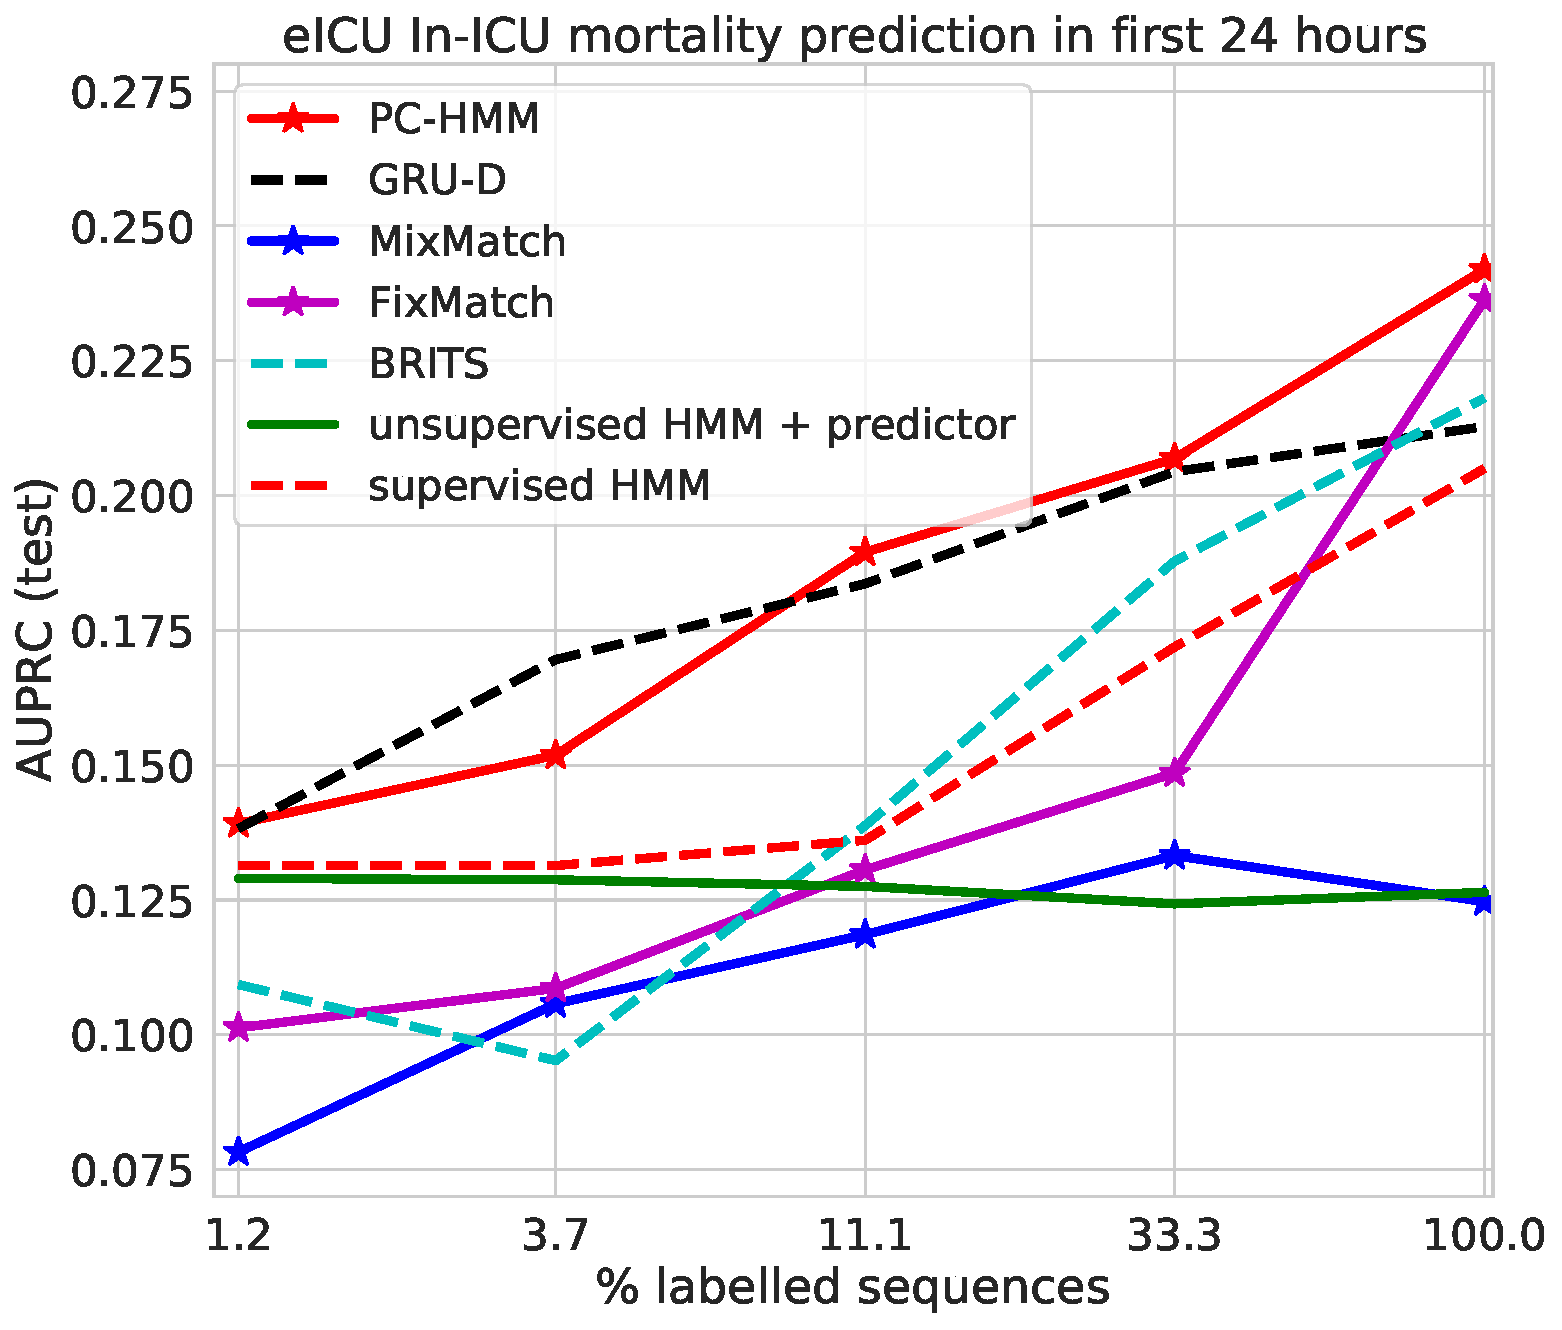
\includegraphics[width=0.5\textwidth]{content/chapters/semi_supervised_pchmm_missing_data/images/perf_mortality_prediction_eicu.pdf}
	&
	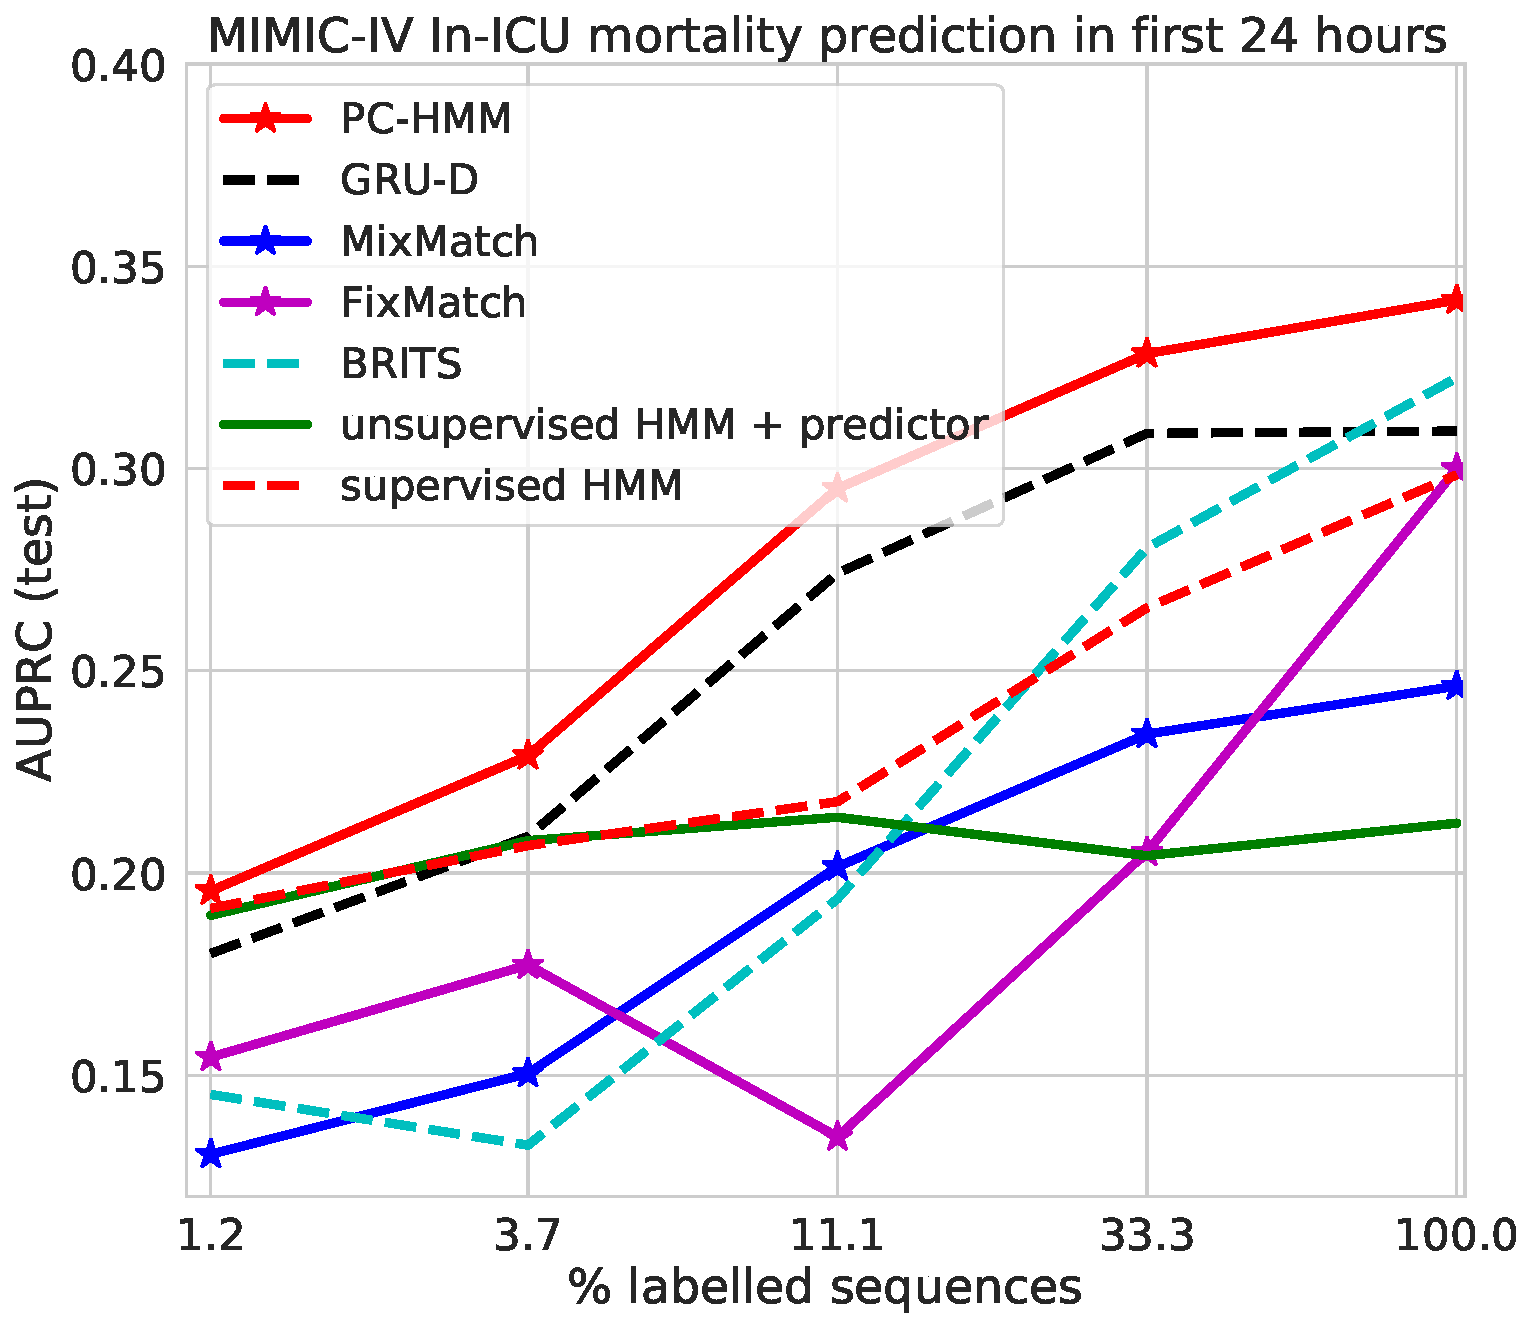
\includegraphics[width=0.5\textwidth]{content/chapters/semi_supervised_pchmm_missing_data/images/perf_mortality_prediction_mimic.pdf}	
\end{tabular}
\caption[AUPRC versus amount of labeled data for in-hospital
mortality early warning classifiers on two large EHR datasets]{AUPRC (higher is better) versus amount of labeled data for in-hospital mortality early warning classifiers on two large EHR datasets (left: eICU, right: MIMIC-IV).
X-axis: Percentage of all training sequences available with labels (SSL methods treat remaining sequences as unlabeled; other methods discard them).
Y-axis: Area under precision-recall curve (AUPRC, higher is better).
%Each line represents a different model.
SSL methods, including our PC-HMM as well as MixMatch and FixMatch,
learn from both labeled and unlabeled data.
GRU-D, BRITS, and Random Forest use the labeled set only.
The PC-HMM matches or beats the other models across all tested labeled set sizes, despite needing fewer parameters and only $1/10^{th}$ of the training time as the other models. }%endcaption

\label{fig:mortality_prediction_results}
\end{figure*}
\subsection{Mortality Prediction Results}
Fig.~\ref{fig:mortality_prediction_results} shows each method's test-set AUPRC (where $y=1$ means death) as label availability $p$ increases.
Across all tested percentages $p$, the PC-HMM is competitive with deep alternatives, including BRITS and GRU-D as well as deep SSL such as FixMatch and MixMatch on both MIMIC and eICU. Notably, the PC-HMM outperforms the baselines with the fewest parameters (see table \ref{table: n_params}), the least training time (see table \ref{table: training_times}) and the fewest number of jobs for hyperparameter search (see table \ref{table: n_params}). The full list of hyperparameters are listed in table \ref{table: hyperparameters}

\begin{table*}[!h]
\begin{tabular}{|l|l|l|l|l|l|l}
\hline
         & \multicolumn{5}{l|}{Confidence Intervals for AUPRC for mortality prediction (100\% labelled)}                                  \\ 
         \hline
         & PC-HMM & GRU-D & MixMatch & FixMatch & BRITS \\ 
         \hline
MIMIC-IV & 0.341 (\scriptsize{0.332, 0.351}) & 0.306 (\scriptsize{0.301, 0.315}) & 0.212 (\scriptsize{0.207, 0.218}) & 0.180 (\scriptsize{0.177, 0.189}) & 0.322 (\scriptsize{0.320, 0.325})  \\ 
\hline
eICU    & 0.243 (\scriptsize{0.239, 0.251}) & 0.211 (\scriptsize{0.209, 0.214}) &  0.126 (\scriptsize{0.120, 0.129})&  0.124 (\scriptsize{0.122, 0.129})&  0.218 (\scriptsize{0.213, 0.220}) \\ 
\hline
\end{tabular}
  \caption[AUPRC with confidence intervals for mortality prediction with all labels known]{AUPRC with confidence intervals for mortality prediction with all labels known. The confidence intervals are obtained by bootstrapping on the test set. We resample 10 different subsets of the test set, and compute AUPRC for each subset. The median (5th, 95th) of the AUPRC across subsets are shown in the table. We find that the variance in prediction across subsets is fairly low and thus only show the performance on the full test set in figures \ref{fig:mortality_prediction_results} and \ref{fig:MIMIC_los_prediction_results}}
    \label{table: CI_performance}
\end{table*}

\begin{table*}[!h]
\begin{tabular}{|l|l|l|l|l|l|}
\hline
Beliefs aggregation  & \multicolumn{5}{l|} {AUPRC for MIMIC-IV mortality prediction varying $p$($\%$ labeled sequences)}\\
\hline
         & $p=1.2$\%      & $p=3.7\%$      & $p=11.1\%$      & $p=33.3\%$      & $p=100\%$     \\
\hline
Average     & 0.19 (\scriptsize{0.18, 0.20})       & 0.23 (\scriptsize{0.22, 0.23})      & 0.29  (\scriptsize{0.29, 0.30})        & 0.32 (\scriptsize{0.32, 0.34})        & 0.34 (\scriptsize{0.33, 0.35})      \\
\hline
1 Conv layer + Max & 0.14 (\scriptsize{0.13, 0.14})       & 0.19 (\scriptsize{0.19, 0.20})      & 0.27  (\scriptsize{0.26, 0.28})        & 0.27 (\scriptsize{0.27, 0.28})        & 0.28 (\scriptsize{0.27, 0.29}) \\
\hline
First + Last Step concat & 0.15 (\scriptsize{0.15, 0.16})       & 0.19 (\scriptsize{0.18, 0.19})      & 0.20  (\scriptsize{0.20, 0.21})        & 0.21 (\scriptsize{0.21, 0.22})        & 0.25 (\scriptsize{0.24, 0.25}) \\
\hline
\end{tabular}
  \caption[Comparison of aggregation strategies of the HMM beliefs, before be-
ing passed as features to the predictor]{Comparison of aggregation strategies of the HMM beliefs, before being passed as features to the predictor. We compare 3 stategies : (1)averaging beliefs across time (2) convolutional transformation of the belief sequence followed by max-pooling \citep{hopePredictionConstrainedHiddenMarkov2021} and (3)concatenating the beliefs at the first and last time steps. Across all levels of missing labels, we observe that averaging the beliefs performs best \citep{sotoodeh2019improving}.}
    \label{table: avg_vs_max_pooling}
\end{table*}

\begin{figure}[!t]
\begin{tabular}{c c}
    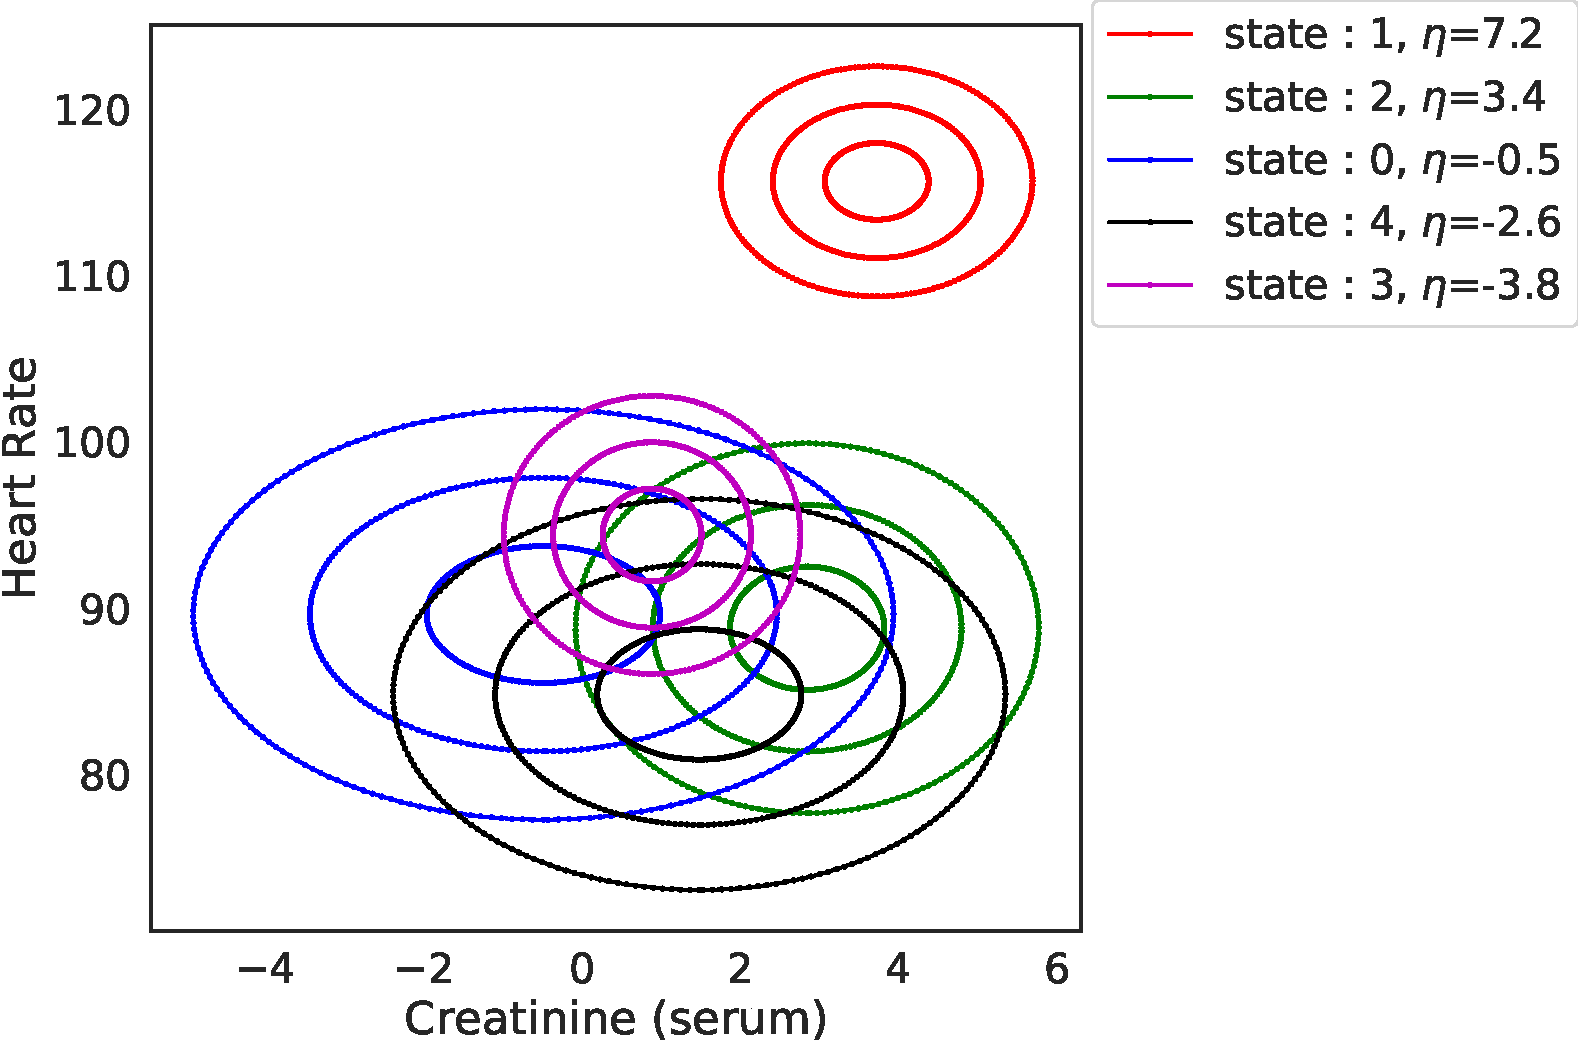
\includegraphics[width=0.5\textwidth]{content/chapters/semi_supervised_pchmm_missing_data/images/interpretability_Heart Rate_Creatinine (serum)_MIMIC.pdf} 
    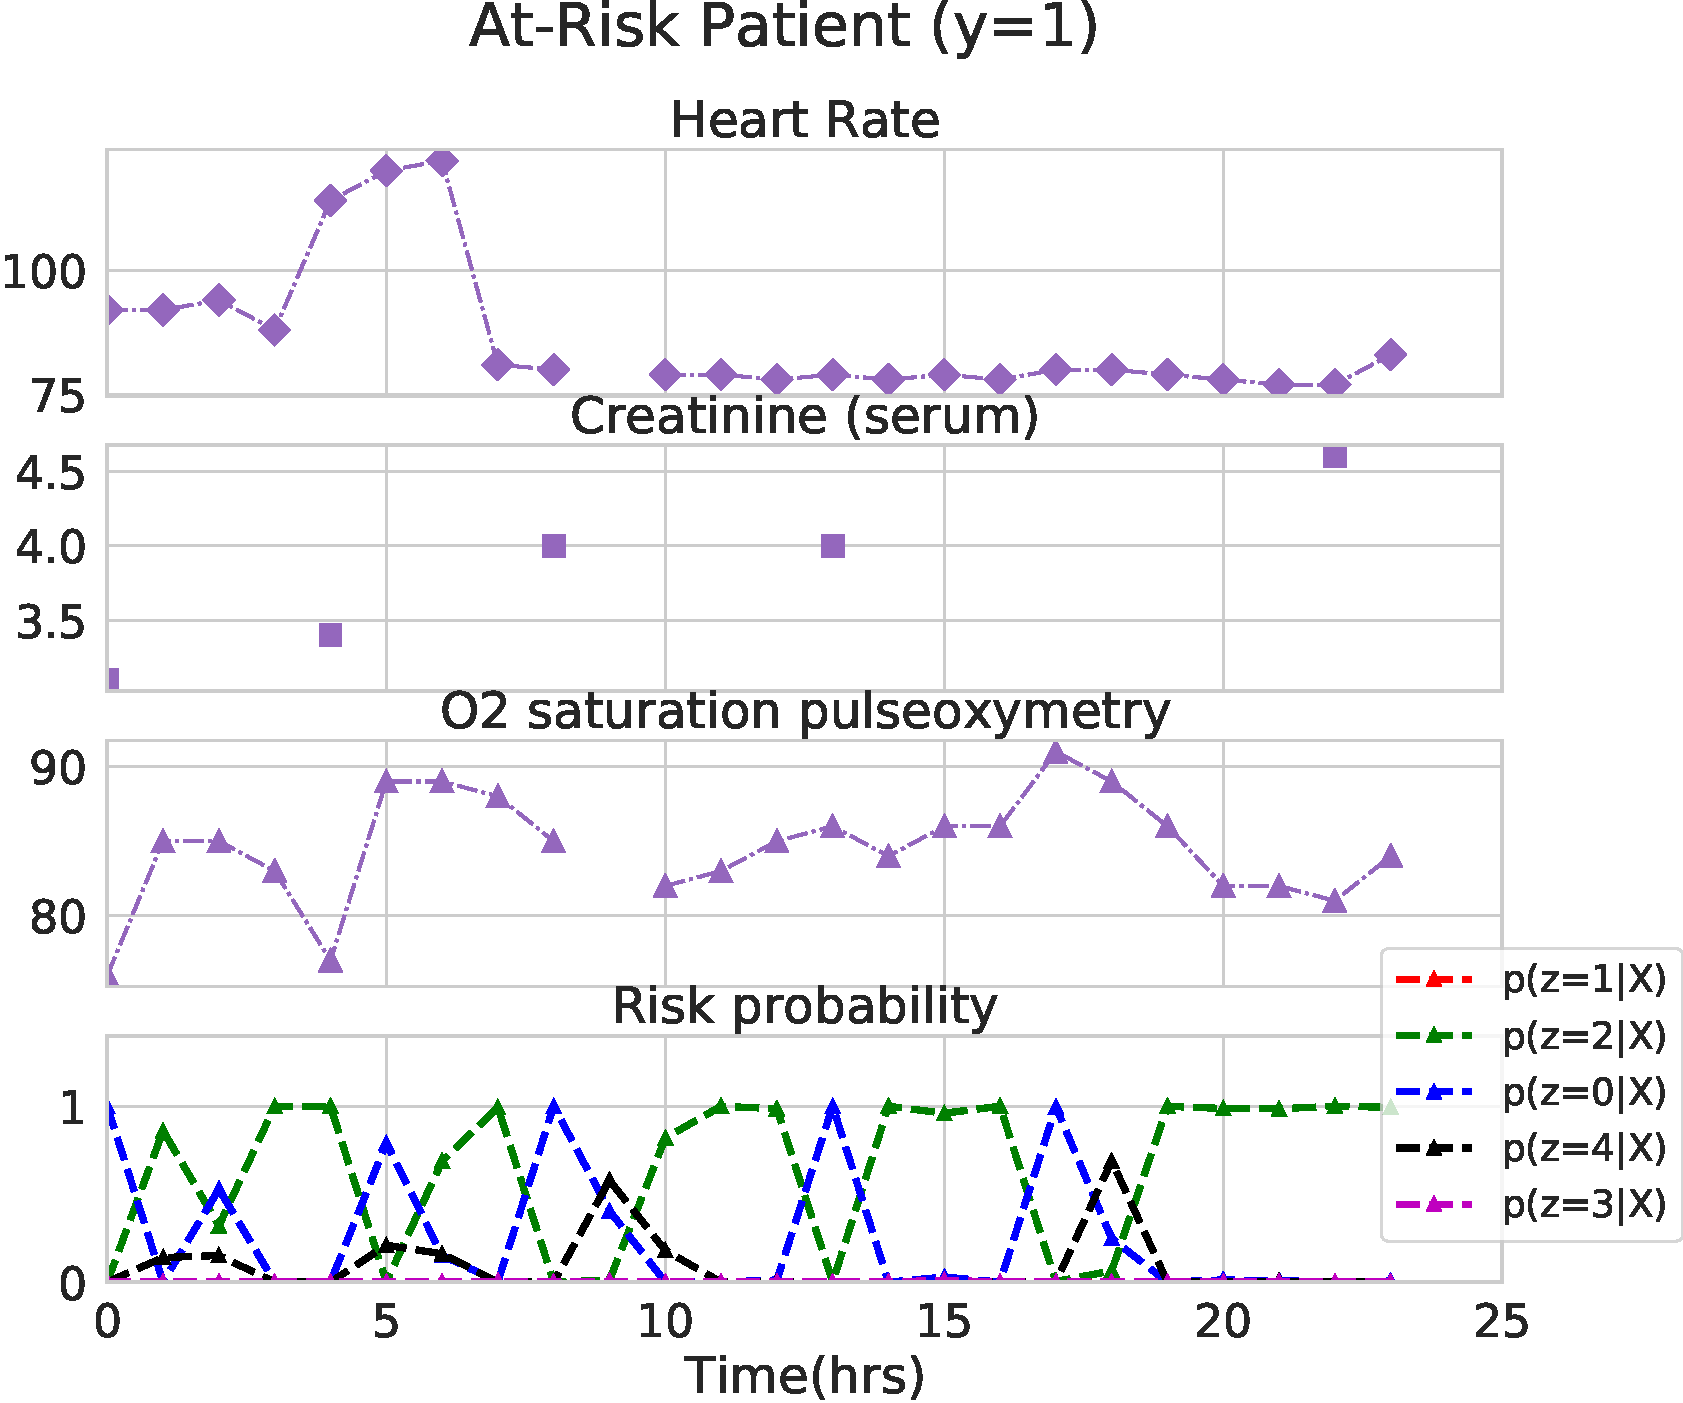
\includegraphics[width=0.5\textwidth]{content/chapters/semi_supervised_pchmm_missing_data/images/mortality_risk_patient_interpretability.pdf} \\
    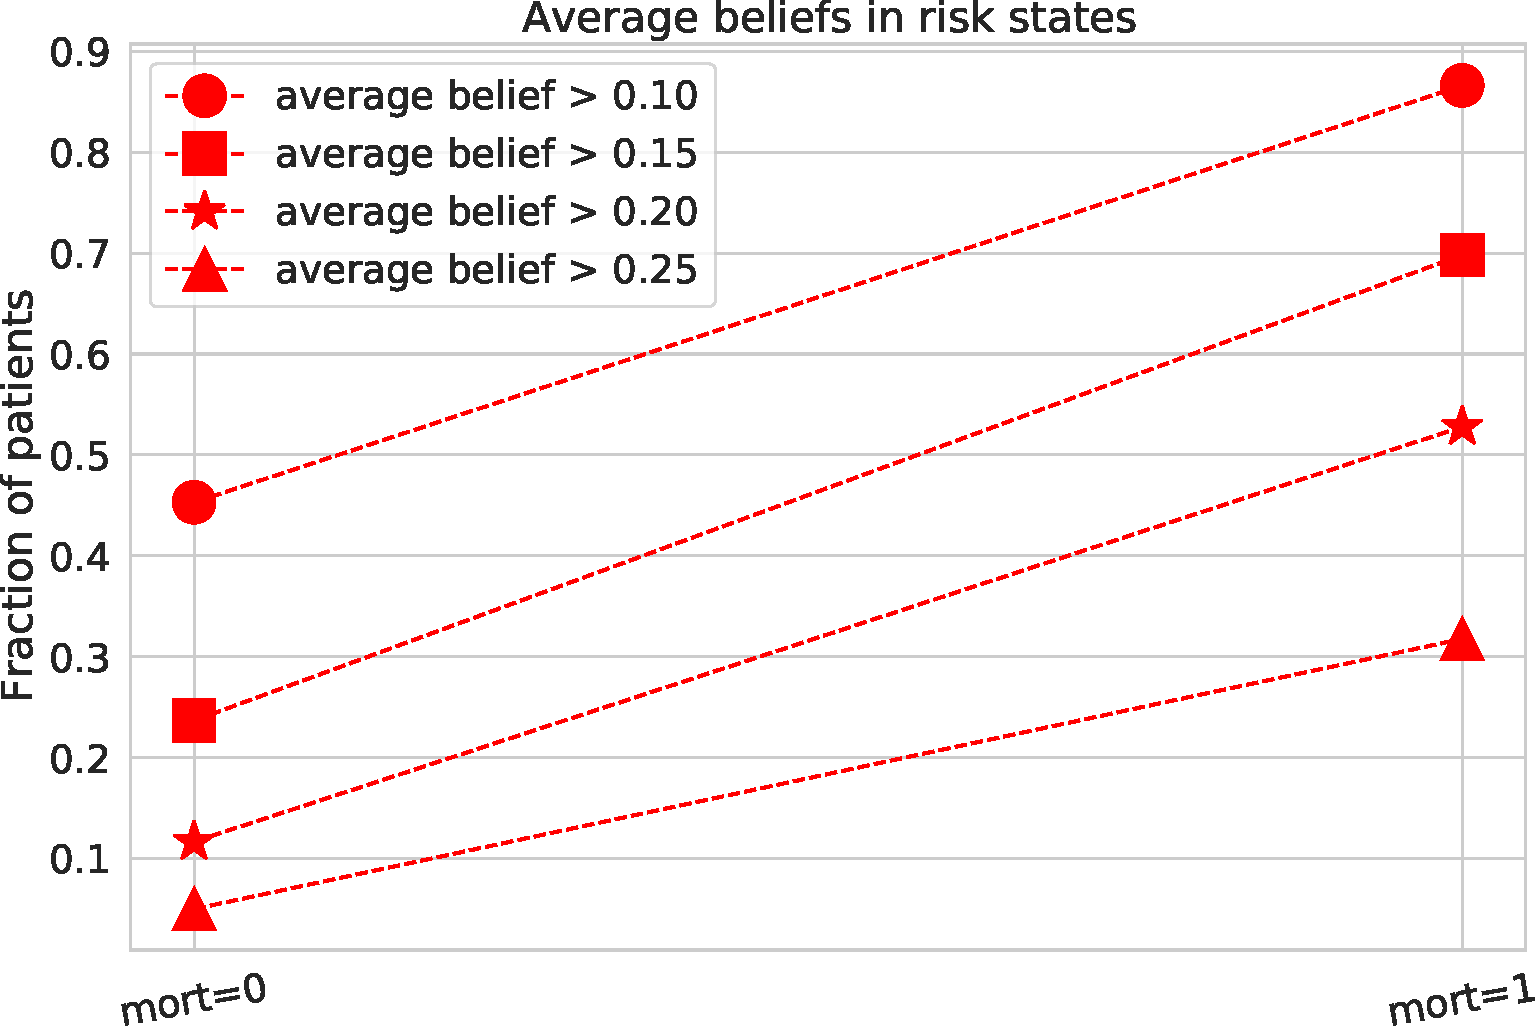
\includegraphics[width=0.5\textwidth]{content/chapters/semi_supervised_pchmm_missing_data/images/avg_beliefs_plots_for_mortality.pdf}
\end{tabular}
\caption[Interpretation of learned PC-HMM for mortality prediction]{
Interpretation of learned PC-HMM on eICU data.
\textbf{\textit{Top Left}}: Gaussian emission distributions of states and their $\eta_k$ (predictor weights).
The red and green states represent high risk (high $\eta_k$).
High risk states seem to represent populations with high heart rate and high creatinine levels (above 1.9mg/dL), which could indicate kidney problems~\citep{baha2021effect}.
\textbf{\textit{Top Right}}: For a patient labeled $y=1$ (who eventually dies), high heart rate and high creatinine are observed throughout the stay, and thus beliefs $b_t$ give highest probability to high risk states.
The probability of state $2$ (green) peak during segments of high creatinine and low oxygen saturation
\textbf{\textit{Bottom}}: We show the average beliefs (averaged over time) of normal patients and risk patients. Clearly, patients at risk spend more time in the risk state compared to the normal patients.
}%endcaption
\label{fig:interpretability_mortality}
\end{figure}

\begin{figure}[!ht]
\begin{center}
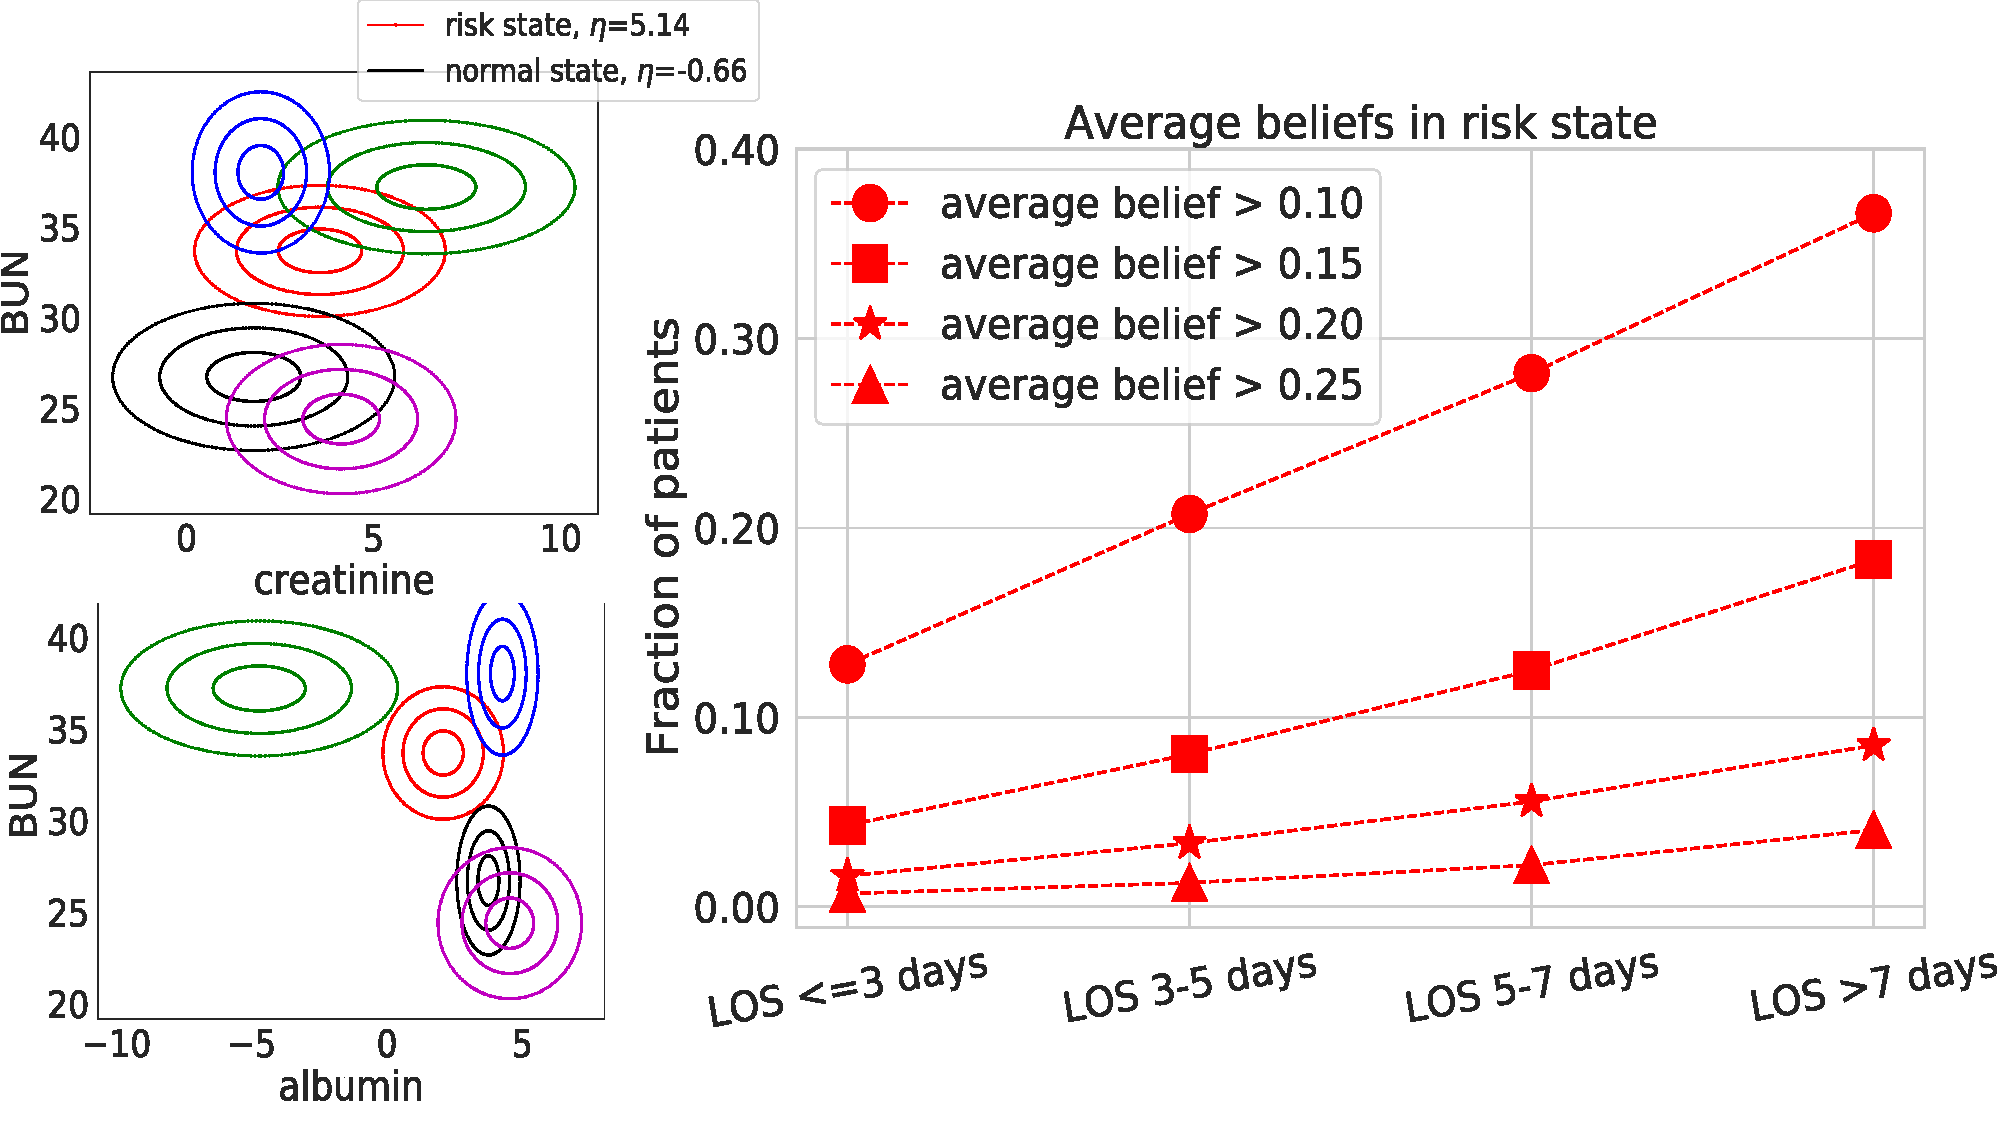
\includegraphics[width=1.0\textwidth]{content/chapters/semi_supervised_pchmm_missing_data/images/interpretability_plot_eicu_2.pdf}
\caption[Interpretability of learned PC-HMM for Length of stay prediction]{\textbf{Left} : Our PC-HMM model reveals five states, representing different risk levels. The red state indicates the `risk state' associated with high BUN and low albumin and high creatinine. \textbf{Right}: We show the average beliefs, averaged over time, in the `risk state'. Notably, as the LOS increases, the average beliefs in the `risk state' increases. 
}%endcaption
\label{fig:interpretability_los_prediction}
\end{center}
\end{figure}

\subsection{Length of Stay Prediction}
Figure \ref{fig:MIMIC_los_prediction_results} plots AUPRC as a function of available labeled data in an SSL setting for MIMIC-IV.
Two major takeaways are apparent.
First, ordinal regression CLMs outperform binary classifiers regardless of whether HMM or neural representations are used.
Second, PC-HMM implementations outperform all other deep learning baselines. Compared to all other baselines, the ordinal regression PC-HMM not only achieves the best performance but also does so with the fewest trainable parameters and lowest training time. 
\begin{figure*}[ht]
\begin{tabular}{@{}c@{\hspace{0.005in}}c@{\hspace{0.005in}}c@{}}
	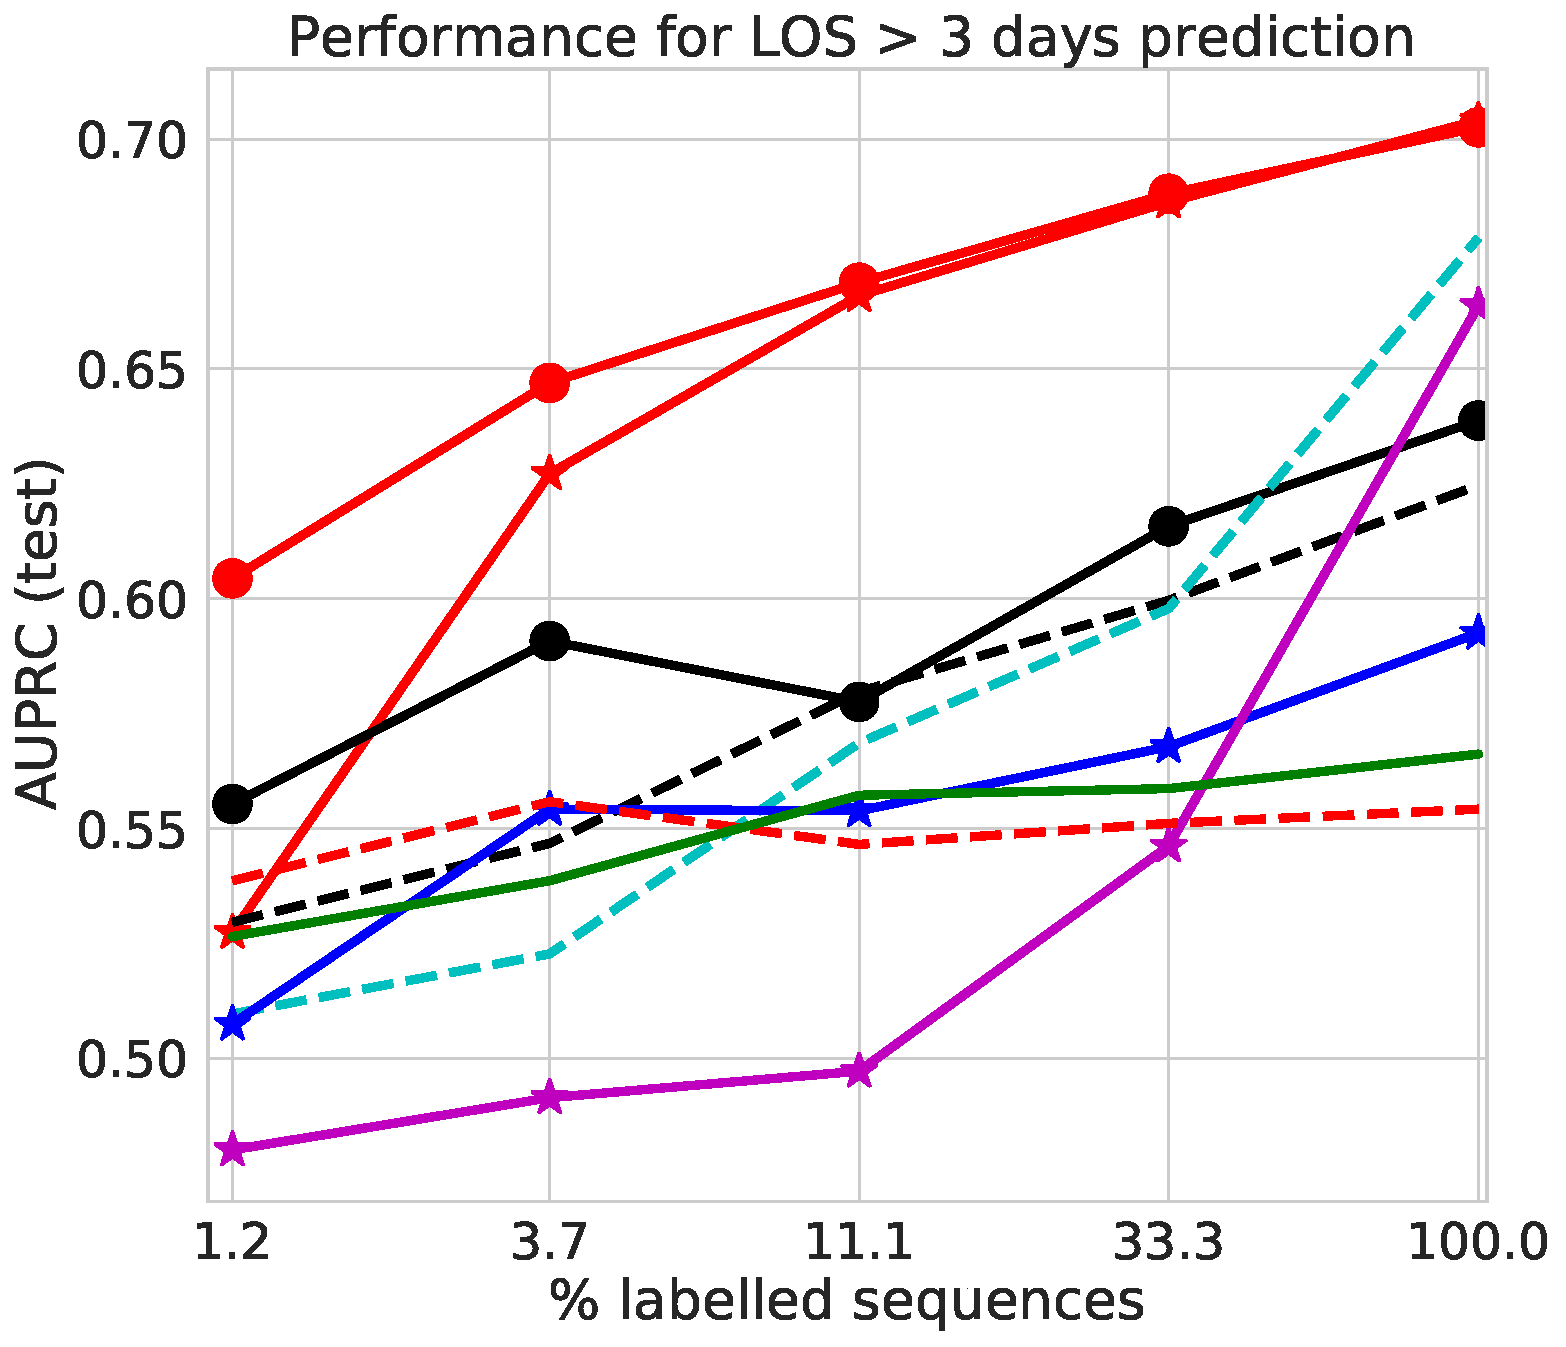
\includegraphics[width=0.35\textwidth]{content/chapters/semi_supervised_pchmm_missing_data/images/perf_los_geq_3_days.pdf}
	&
	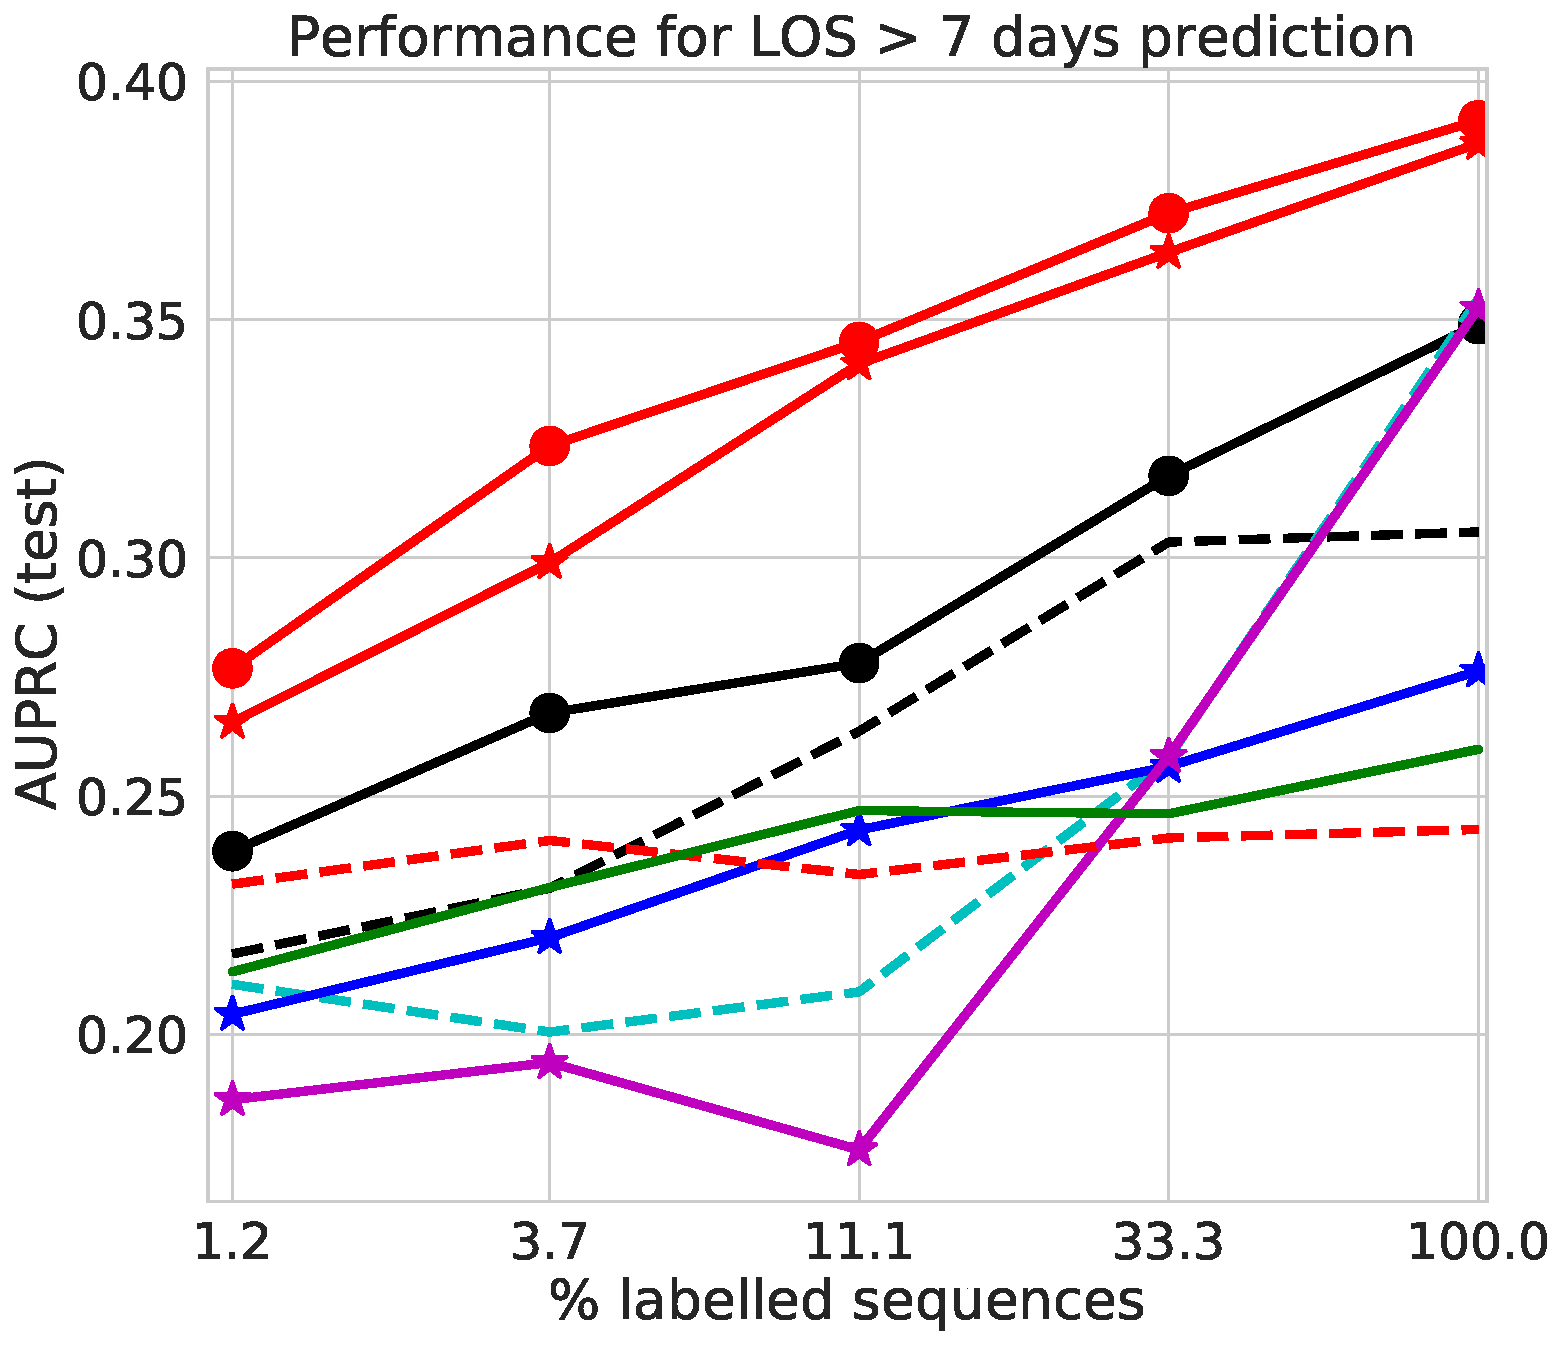
\includegraphics[width=0.35\textwidth]{content/chapters/semi_supervised_pchmm_missing_data/images/perf_los_geq_7_days.pdf}	
 	&
	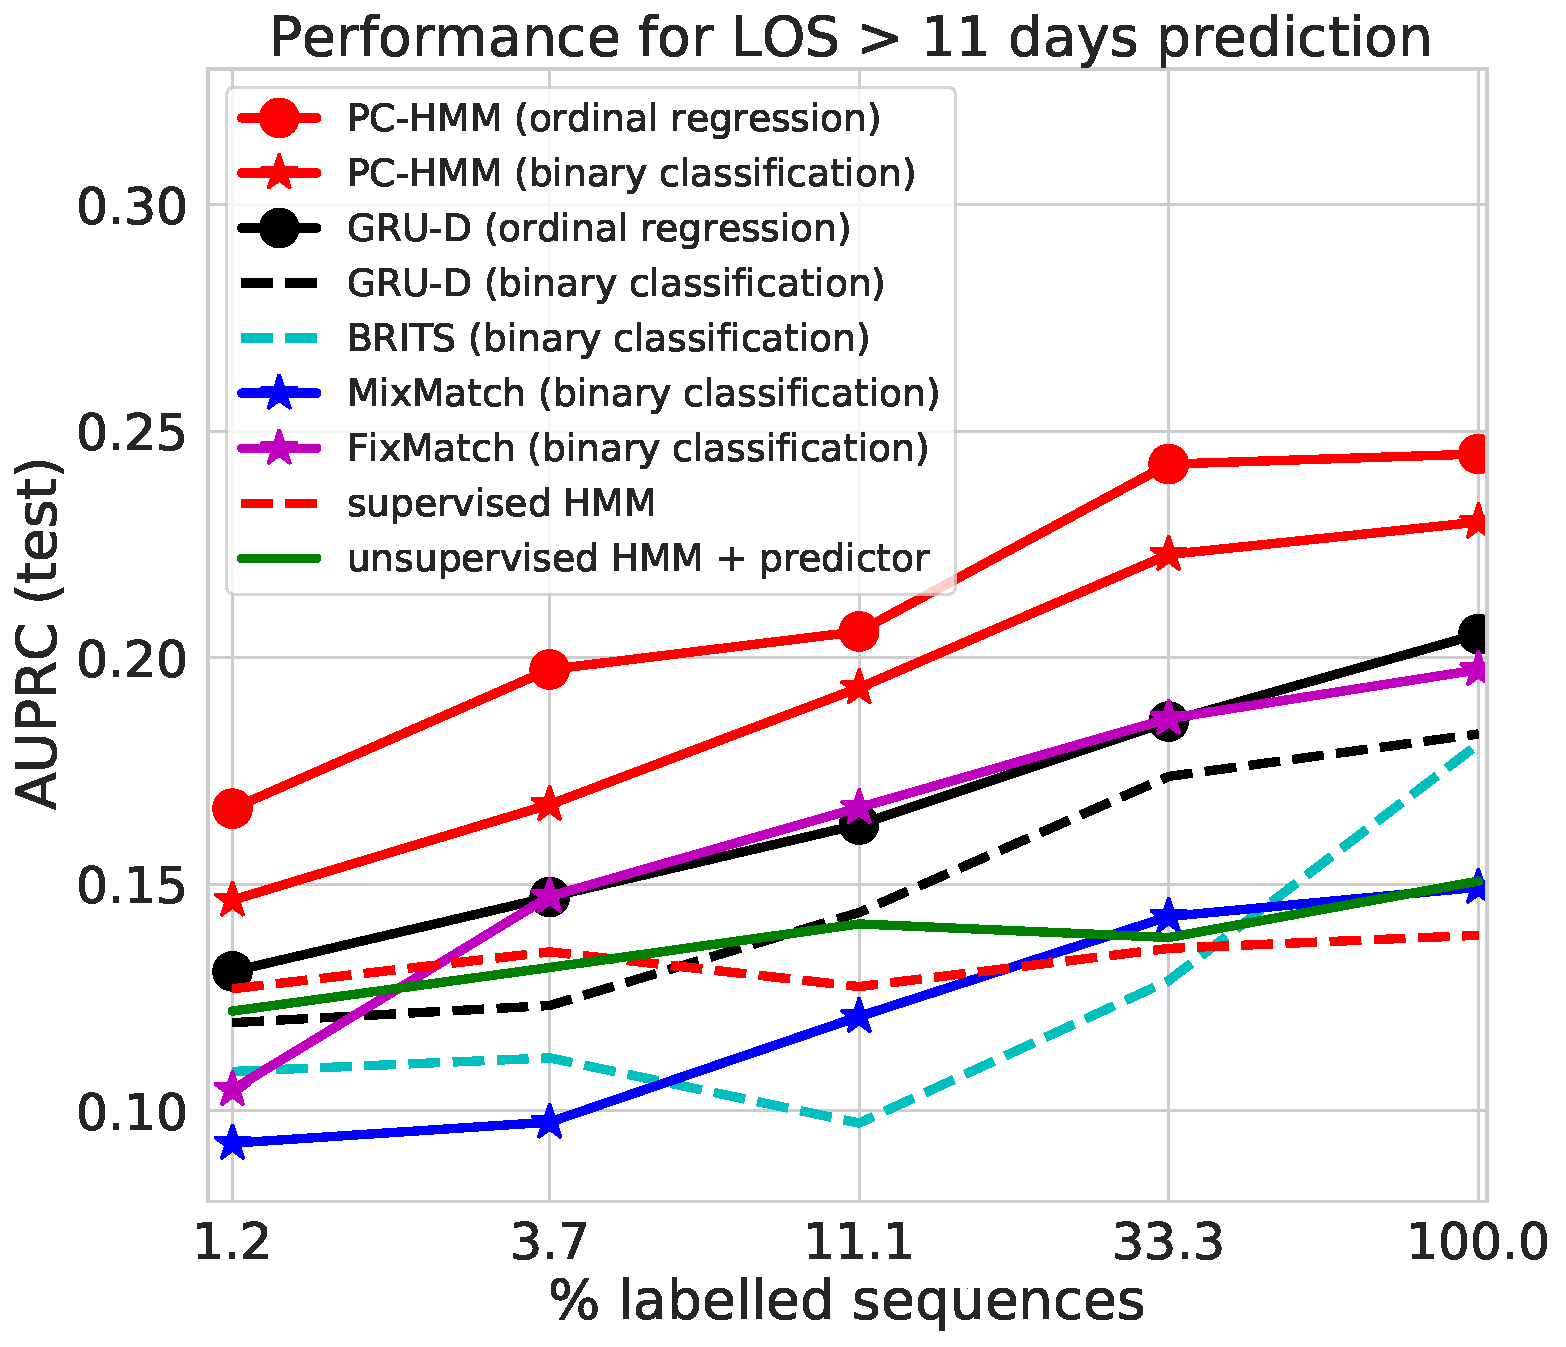
\includegraphics[width=0.35\textwidth]{content/chapters/semi_supervised_pchmm_missing_data/images/perf_los_geq_11_days.pdf}	
\end{tabular}
\caption[AUPRC versus amount of labeled data for length-of-stay prediction on MIMIC-IV at 3 ordinal labels ($>3$, $>7$, and $>11$ days)]{AUPRC (higher is better) versus amount of labeled data for length-of-stay prediction on MIMIC-IV at 3 ordinal labels ($>3$, $>7$, and $>11$ days).
SSL methods (PC-HMM, MixMatch, and FixMatch)
learn from both labeled and unlabeled data.
GRU-D \citep{cheRecurrentNeuralNetworks2018} and BRITS \citep{caoBRITSBidirectionalRecurrent2018} use the labeled set only.
Binary classification models require 3 separate models (1 for each label), whereas ordinal regression using CLMs require a single model to predict all 3 labels. }%endcaption
\label{fig:MIMIC_los_prediction_results}
\end{figure*}

\input{content/chapters/semi_supervised_pchmm_missing_data/fig_results_eicu_los_prediction}


\subsection{Interpretation of Learned PCHMM States}
Our PC-HMM framework enables us to interpret cohorts of vulnerable populations by visualizing the emission distributions for the states that have the highest predictor coefficients $\eta_k$.
% Some of these cohorts from eICU are visualized in Figure \ref{fig:interpretability}. 
On eICU data, Fig.~\ref{fig:interpretability_mortality} shows our PC-HMM identifies states representing high blood urea nitrogen (BUN) and high creatinine (common indicators of kidney failure \citep{baha2021effect}) as the most vulnerable to in-ICU mortality. 
The model transitions to these `high-risk' states as soon as high values of creatinine and BUN are observed in a patient who eventually dies.
Additionally, we illustrate the interpretability of the PC-HMM trained to predict length of stay in Figure \ref{fig:interpretability_los_prediction}, highlighting that longer stays are associated with larger beliefs in the `risk state'.


\subsection{Training times for each model}
\begin{table}[H]
\centering
\begin{tabular}{|l|l|l|l|l|l|l|}
\hline
 & & \multicolumn{5}{l|}{\textit{seconds/epoch} to train each model} \\
\hline
    Dataset & & PC-HMM & GRU-D & MixMatch      & FixMatch      & BRITS     \\
\hline
MIMIC-IV & $D=41$ features & 9   & 43       & 70         & 55         &  48     \\
\hline
eICU    & $D=41$ features & 16        & 70       & 115         & 90   &  75     \\
\hline
\end{tabular}
  \caption[Computation time (seconds/epoch) required per model]{Computation time (seconds/epoch) required by each model. An epoch is completed when every example in the training set is covered at-least once. Although computation time increases when measurements are more frequent, the PC-HMM still requires far lesser time to train due to significantly lesser parameters than the other models.}
    \label{table: training_times}
\end{table}

\subsection{Parameter counts and Hyperparameter search for each model}
\begin{table}[H]
\centering
\begin{tabular}{|l|l|l|l|l|l|}
\hline
     & PC-HMM & GRU-D & MixMatch  & FixMatch      & BRITS     \\
\hline
Parameters & 452-2,102  & 12,739-87,523   & 2,866-45,634  & 2,866-45,634  &  48,850-252,370     \\
\hline
Jobs & 900 & 7,560 & 10,800 & 21,600 &  6,480     \\
\hline
Training time(per job) & 1-2 hrs & 5-6 hrs & 6-8 hrs & 4-6 hrs &  4-5 hrs  \\
\hline
\end{tabular}
  \caption[Range of parameter counts and number of jobs for hyperparameter search per model]{Range of parameter counts and number of jobs for hyperparameter search for each model. The PC-HMM requires the fewest parameters, least number of jobs for hyperparameter search, and the least training time and yet produces the best performance.}
    \label{table: n_params}
\end{table}

\newcommand{\tabitem}{~~\llap{\textbullet}~~}
\begin{table*}[!t]
  \centering
  \begin{tabular}{|l|l|l|}
    \hline
    Model & Hyperparameters searched & Selection criterion\\
    \hline
    PC-HMM & \tabitem learning rate : $0.001, 0.01, 0.1$ & Best validation AUPRC  \\
    & \tabitem states : $5, 10, 20$ & \\
    & \tabitem initialization seeds : 5 & \\
    & \tabitem l2 penalty : $0, 0.01, 0.1, 1$ & \\
    & \tabitem $\lambda$ : $50, 100, 500, 1000, 5000$ & \\
    \hline
    GRU-D & \tabitem learning rate : $0.001, 0.01, 0.1$ & Best validation AUPRC \\
    & \tabitem hidden units : $32, 64, 128$ & with early stopping \\
    & \tabitem hidden layers : $1, 2$ & \\
    & \tabitem initialization seeds : 20 & \\
    & \tabitem l2 penalty : 7 log-spaced values between $10^-6$ and $100$ & \\
    & \tabitem batch-size : $128, 256, 512$ & \\
    \hline
    BRITS & \tabitem learning rate : $0.001, 0.01, 0.1$ & Best validation AUPRC\\
    & \tabitem hidden units : $32, 64, 128$ & with early stopping \\
    & \tabitem initialization seeds : 20 & \\
     & \tabitem hidden layers : $1, 2$ & \\
    & \tabitem dropout : $0, 0.1, 0.25$ & \\
    & \tabitem batch-size : $128, 256, 512$ & \\
    & \tabitem imputation-weight : $0.3, 0.6$ & \\
    & \tabitem label weight : $1.0$ & \\
    \hline
    FixMatch & \tabitem learning rate : $0.001, 0.01, 0.1$ & Best validation AUPRC \\
    & \tabitem hidden units : 16, 32, 64 & with early stopping \\
    & \tabitem initialization seeds : 5 & \\
    & \tabitem hidden layers : $1, 2$ & \\
    & \tabitem batch-size : $128, 256, 512$ & \\
    & \tabitem l2 penalty : 5 log-spaced values between $10^-8$ and $10$ & \\
    & \tabitem pseudo-label thresholds : $0.6, 0.8$ & \\
    & \tabitem augmentation noise variance : $0.1, 0.01$ & \\
    & \tabitem unlabeled strength : $50, 75$ & \\
    & \tabitem Temperature scaling : $0.5$ & \\
    & \tabitem $\alpha$(for MixUp): $0.75$ & \\
    \hline
    MixMatch & Same hyperparameter grid as FixMatch & Best validation AUPRC \\
    & except no psuedo-label thresholds & with early stopping\\
    % \hline
    % Random Forest & \tabitem Fraction of  features : $0.33, 0.66, 1.0$ & Best validation AUPRC \\
    % & \tabitem Max leaf nodes : 32, 64, 128 & \\
    % & \tabitem Min Samples per leaf : 64, 128, 512, 1024 & \\
    % & \tabitem Estimators : 64 & \\
    \hline
  \end{tabular}
  \caption{Hyperparameters for all the models}
  \label{table: hyperparameters}
\end{table*}
\section{Conclusion}
In order to address the growing need to predict reliable LOS outcomes from patient data, we have presented a model that not only outperforms alternatives but also does so with minimal parameters. By taking advantage of the smooth likelihood for ordinal data, we show how the cumulative link framework may be incorporated into any model trainable with gradient descent. When incorporated into the PC-HMM, we observe how generative and discriminative goals are balanced to effectively predict LOS in both fully- and semi-supervised cases. Unlike other candidates for ordinal regression, this established framework maintains a monotonically increasing probability for subsequent ordinal classes that are grouped together. This, along with their loss convexity, make CLMs an ideal candidate to address the novel problem of predicting hospital stays. Promising results on patient time-series datasets exhibit the utility of this model. We plan to explore further use cases such as characterizing disease severity with medical data.

\chapter{Probabilistic Modeling of Data-Driven Missingness in Irregular Time Series Medical Records}
\section{Introduction}
In this chapter, we consider the problem of modeling a time series of several variables gathered at irregularly-spaced times, especially when only a few variables are typically measured at one time. Our motivating application is to model the sequence of vital signs and laboratory values recorded over time in the EHR of a hospitalized patient. Effective models of such data could enable many improvements to both patient care and hospital logistics, such as extrapolating the future state of the patient, facilitating diagnosis of underlying illness, or crafting personalized treatment strategies~\citep{hyland2020early, bica2021real}. 

Realizing these benefits requires a model that can handle the two key aspects of our chosen scenario. First, the model must accommodate the \emph{irregular timing of individual measurements}. Second, the model must capture the \emph{data-dependent patterns of missingness}. To clarify this latter point, whether a specific variable is measured or not in the present moment is often influenced by current or recent measurements of other variables. Intuitively, doctors rarely order lab tests unrelated to the patient's present condition or medical history.

We focus on a specific technical formulation of the generative mechanism for missingness, known as \emph{missing at random} (MAR) \citep{rubin1976inference}. In MAR settings, the presence or absence of a measurement variable (binary indicator of missingness) depends on the values of all observed (non-missing) variables. As one example of MAR, the current value of Troponin, an indicator of heart failure measured via lab processing of a blood draw, could be missing due to other observed vitals indicating normal heart function. As another example, the absence of cholesterol measurements could be attributed to the lack of evident risk factors for heart disease, alongside a normal weight and healthy Body Mass Index (BMI). In contrast to MAR, the  commonly assumed \emph{missing completely at random} (MCAR) setting assumes the missingness indicator arises independently of any observations.

Unfortunately, many common models for time-varying labs and vitals are not capable of handling both irregular timing and data-driven (MAR) missingness assumptions.
Well-known recurrent neural nets for clinical time-series, such as GRU-D~\citep{che2018recurrent} or BRITS~\citep{caoBRITSBidirectionalRecurrent2018}, do allow for arbitrary missingness at each timestep at both training and prediction.
However, these methods assume regular time intervals, necessitating alignment to a uniformly-spaced time grid as a pre-processing step.
%Furthermore, these methods assume MCAR rather than MAR mechanisms.
Another growing line of work directly models irregularly timed measurements via continuous formulation of recurrent networks \citep{pineda1987generalization, pearlmutter1989learning} and more recently via neural networks coupled with differential equation solvers \citep{de2019gru, rubanova2019latent}. However, in these works (as well as works like GRU-D and BRITS) there is no focus on a data-dependent (MAR) missingness mechanism. The current landscape thus lacks a method that can simultaneously handle irregular-spacing and data-dependent missingness.

In this work, our \textbf{primary contribution} is a method that fills this gap. We present a probabilistic generative model for an irregular time series of clinical measurements with an data-driven mechanism that allows arbitrary missingness at any time. 
Irregularly-spaced measurements are handled via an encoder-decoder stochastic differential equation architecture known as the continuous recurrent unit (CRU)~\citep{schirmer2022modeling}. Data driven missingness is handled via regression on time-specific representation vectors produced by the CRU. Our approach  preserves the efficient closed-form updates inside the CRU.

We demonstrate the effectiveness of our approach by examining prediction error
when \emph{extrapolating} the next few hours of a patient's multivariate time series. Across 3 real health records datasets, each containing thousands of patients, we show our approach delivers lower extrapolation error (averaged across 12+ labs and vitals) than several state-of-the-art alternative methods designed for irregularity but not data-dependent missingness. Further sensitivity analyses on synthetic data confirm that our advantage occurs specifically in settings where the MCAR assumptions of baselines are not appropriate.
While our evaluations focus on EHRs for hospitalized patients, our method design is general purpose and useful for any time-series modeling that needs both irregular time and data-dependent missingness.

As a \textbf{contribution to best practices in evaluation}, our experiments report two kinds of error. First, we report
average error across all channels after normalization (as many past works do). Second, we report channel-specific error without normalization, using the raw units of the original physiological measurement. This latter approach is not routinely done in other works, but we find it is valuable way to contextualize our method's gains.


\subsection*{Generalizable Insights about Machine Learning in the Context of Healthcare}

Our work highlights the importance of careful joint modeling of missingness and measured values, using a data-driven (MAR) mechanism, while also accounting for the irregularly-spaced nature of EHR records over time. The choice of what to measure and when carries critical information that can be used to improve understanding of the patient's condition. Hopefully this improved understanding and ability to forecast future patient state could help lead to improved treatment decisions and better outcomes.

\section{Prior Work}
Below, we review several lines of work addressing either missingness or irregular timing.

~\\ \noindent
\textbf{Types of missingness.}
Foundational work in defining the 3 different missing data scenarios MAR (missing at random), MCAR (missing completely at random) and MNAR (missing  not-at random) was done by \citet{rubin1976inference}. 
We situate our proposed model in the MAR category.

~\\ \noindent \textbf{Missngness and deep generative models.} 
\citet{mattei2019miwae} introduced an approach for training deep generative models using importance weighted autoencoders (IWAE) under MAR assumptions. \citet{ipsen2020not} extended that work to cover MNAR assumptions with their not-MIWAE method, which was later specialized to supervised tasks~\citep{ipsen2022deal}. 
Another model called GINA, introduced by \cite{ma2021identifiable} provides identifiability guarantees 
%under mild assumptions, 
for a wide range of MNAR mechanisms. All these works assume  \emph{static} data and are not designed to handle time series. 

~\\
\noindent \textbf{RNNs for regular time series with missing data.} Several prior works tackle missing values with variants of recurrent neural networks (RNNs). \cite{liptonModelingMissingData2016} feed missing value indicators as additional inputs to the model together with forward-fill imputation to enable the model to learn 'real' vs 'filled-in' values. \cite{che2018recurrent} proposed the GRU-D, which extends the well-known GRU architecture \citep{cho2014properties} by incorporating a trainable decay that imputes missing features in a way that interpolates over time between two strategies: forward-fill and the population mean. GRU-D allows the time since the last observation to impact representations in a way that usual regular-grid RNNs do not. However, their experiments required an input time series aligned to a regularly spaced grid.
\cite{caoBRITSBidirectionalRecurrent2018} designed a bidirectional RNN called BRITS that performs imputation and classification/regression jointly in one neural graph. \cite{futomaLearningDetectSepsis2017} proposed a hybrid approach which uses a Gaussian process to impute values which are later fed into an RNN.
More recently, \cite{kim2023probabilistic} proposed a probabalistic  model for regularly spaced time-series with a missing not at random assumption. They extend the not-MIWAE deep generative model \citep{ipsen2022deal} to time-series with a GRU backbone and introduce a novel regularization strategy to enable learning missing values for better downstream classification. Unlike all of these methods, our model does not rely on aligning data to a regularly spaced grid, thereby enabling learning from the raw irregularly spaced time-points.  

~\\
\noindent \textbf{Models for irregular time-series.}
Models for irregular time series belong to several types: (1) interpolation-based models and (2) ODE/SDE-based models, (3) Graph based models, (4) Diffusion based models, (5) Large language models (LLM) based models discussed below and (6) Tensor factorization based models

\emph{Interpolation-based models.} \citet{shukla2019interpolation} propose a semi-parametric  interpolation network where irregularly spaced observations are interpolated to a grid of regularly spaced timepoints before prediction with any standard downstream predictor. \citet{li2020learning} propose an encoder-decoder architecture where the irregularly sampled time-series is assumed to be sampled from a continuous unobserved function. The encoder is a continuous convolution layer to accommodate irregularly sampled inputs, while their decoder uses a kernel smoother to learn a function over a reference set of uniformly spaced times. \cite{shukla2021multitime} propose an attention-based model that converts the irregular time series to a regular grid before prediction. 
%They use a multi time attention model with query time point $t$ and a set of keys and values in the form of a $D$-dimensional multivariate sparse and irregularly sampled time series. 
For all these models, missing values are zero-encoded before training. There is no emphasis on data-dependent missingness.

\emph{ODE/SDE-based models.} \citet{rubanova2019latent} propose a generative model where the latent state is driven by a latent ordinary differential equation (ODE).  
\citet{kidger2020neural} extends that work via a neural-controlled differential equation instead of an ordinary differential equation. 
This allows the model to update the latent state trajectory with incoming observed data. \cite{de2019gru} extends the GRU architecture to incorporate input from an ODE, also in a way that allows observations to influence the latent trajectory. A similar ODE based model has also been proposed by \citet{jia2019neural}.
\cite{chauhan2022coper} extend the continuous state perceiver network \citep{jaegle2021perceiver} to learn the continuous dynamics of a patient, requiring 2 ODE solvers. 
All these works require expensive numerical solvers for training and prediction.

\emph{Graph-based models.} 
\citet{zhang2021graph} introduced RAINDROP, a graph neural network that handles asynchronous and irregularly recorded observations from multiple sensors. It considers sensor dependencies for message passing and generates multi-scale embeddings using hierarchical attention. However, the model estimates missing values using observational embeddings from neighboring vertices without learning a probabilistic model for missingness. Further, it is hard to assess the quality of imputations by their model, since only classification performance on downstream tasks are presented.

\emph{Diffusion based models.}
\citet{tashiro2021csdi} propose a score-based diffusion model trained via self-supervision and is conditioned on observed data for imputation. While their model claims to reduce absolute errors by a $5-20\%$ margin compared to other models, their evaluation depends on intricate adjustments to the denoising function and a self-supervised learning strategy that separates observed values into conditional information and imputation targets for training.

\emph{Large language models.} Recently, \citet{gruver2023large} demonstrated that zero-shot extrapolation with Large Language Models (LLMs) outperform numerous time-series forecasting baselines in performance. However, their approach forecasts each dimension independently and ignores the actual timestamps of measurements. This limitation renders their model ineffective for datasets containing irregular timestamps and correlations between channels. We add the LLMTime baseline to our toy data experiment in Figure \ref{fig:models_generated_seq} and highlight the poor extrapolation performance on synthetic data.

\emph{Tensor factorization based models.} \citep{yin2020logpar} introduced Logistic PARAFAC2, a model designed to handle binary data with missing values by using Bernoulli distributions and a positive-unlabeled learning loss function. This approach improves tensor completion and predictive performance by incorporating uniqueness and temporal smoothness regularization. However, their MIMIC-III dataset is constructed on an eight-hour basis by accumulating clinical features in consecutive time windows. This may not capture all relevant temporal dynamics and could limit the applicability to clinical features that vary within shorter time frames.

~\\ \noindent
Our work directly builds upon the continuous recurrent unit (CRU) by \citet{schirmer2022modeling}. 
%The CRU is designed to perform representation learning for irregular time series. 
As detailed in Sec.~\ref{sec:CRU}, the CRU is an SDE-based method for representation learning on irregular time series.
Hidden representations evolve via a linear time-invariant stochastic differential equation (SDE), with encoder/decoder mappings for added flexibility. 
However, the off-the-shelf CRU model does not model \emph{missingness} at all. Our proposed method extends the CRU to handle data-dependent missingness scenarios.
Recent work by \citet{ansari2023neural} propose a neural continuous discrete state space model (NCDSSM). This is similar to the CRU but it avoids the CRU's restriction to linear time-invariant SDEs. Again, that work does not address learning  missing mechanisms.
\newcommand{\MExp}{{\small \textsc{MExp}}}
\section{Background}
Here, we review the technical problem we are trying to solve as well as the details of \citet{schirmer2022modeling}'s
continuous recurrent unit (CRU). 
This lays a conceptual foundation for our later innovations that incorporate data-dependent missingness mechanisms in Sec.~\ref{sec:CRU_gen_model}.


\paragraph{Problem: Irregular time series with missingness.}
We consider building a model for many multivariate sequences.
%For each sequence, we first define $t_0$ as a special reference start time for each sequence (e.g. the moment of admission to the hospital).
For each sequence, we have observations at a set $\Gamma$ of $L$ distinct irregularly-spaced observation times: $\Gamma=\{ t_1, ..., t_L\}$, which we assume are sorted in ascending order and are all greater than a reference start time $t_0$.

We also have a sequence $\mathbf{x}$ of observed feature vectors, one for each observed time: $\mathbf{x} = \{x_t : t \in \Gamma \}$. 
Each feature vector $x_t \in \mathbb{R}^D$ represents measurements of a fixed set of $D$ variables (sometimes called channels). There may be arbitrary missingness in each $x_t$. 
Let $s_t \in \{0, 1\}^D$ be a binary indicator vector of size $D$ indicating whether a variable is ``seen'' (observed) or not (missing). That is, $s_{td} = 1$ if $x_{td}$ is observed and 0 otherwise.

\subsection{Continuous Recurrent Unit (CRU)}
\label{sec:CRU}

A core building block of our approach is the continuous-time recurrent unit (CRU) by \citet{schirmer2022modeling}. The purpose of the CRU is to provide a  mapping from a \emph{non-missing} irregular time series of length $L$ to a output sequence of representation vectors of the same length $L$. We write the CRU as
\begin{align}
    [h_{t_1} \ldots h_{t_L}], [\tau_{t_1} \ldots \tau_{t_L}] \gets \textsc{CRU}(x_{t_1} \ldots x_{t_L}, \Gamma).
    \label{eq:CRU_as_RNN}
\end{align}
At each observation time $t_\ell$, the CRU produces two $D$-dimensional vectors $h_{t_{\ell}}, \tau_{t_{\ell}}$. That is, $|h_t|{=}|\tau_t|{=}|x_t|{=}D$ for all $t \in \Gamma$. Vector $h_{t_\ell}$ is can be thought of as a decoded representation for data $x_{t_\ell}$.
Vector $\tau_{t_L}$ is meant to encode uncertainty about each data dimension.
%the representation vector and $\tau_t$ represents the uncertainty in the representations at time $t$.

We stress that the CRU as presented by \citet{schirmer2022modeling} assumes that each $x_t$ is fully observed, without any missingness. While they offer a zero-filling heuristic to accommodate missingness, our later experiments show this is inadequate for downstream predictions when data is missing-not-at-random. Instead, our methods in Sec.~\ref{sec:CRU_gen_model} provide an explicit mechanism to handle the data-dependent missingness scenarios.

\paragraph{CRU overview.}
The CRU produces representations via continuous-discrete Kalman-filter forward inference \citep{jazwinski2007stochastic} for a latent variable time-series model.
Internally, the CRU assumes two time-varying continuous random variables: a $M$-dimensional latent vector $z_t$, and a $C$-dimensional encoded feature vector $y_t$. Latent $z_t$ has a \emph{prior} distribution specified by a stochastic differential equation (SDE) model for $z_t$ as a function of $t$.
When this SDE assumes a Gaussian noise process, this ultimately yields a Gaussian prior with time-varying parameters.
%to a linear operation on the noise process
%The solution to the prior SDE in Eq.~\eqref{eq:LTI_SDE_soln} is a Gaussian distribution due to a linear operation on the noise process (which is itself Gaussian).  
We then define a Gaussian \emph{likelihood} that produces encoded features $y_t$ given latent $z_t$. Due to conjugacy between the solution to the prior SDE and the likelihood, \citet{jazwinski2007stochastic} shows that the posterior over $z_t$ given previously observations, $p( z_t | \{y_u : u < t, u \in \Gamma \})$, remains Gaussian with closed-form mean and covariance.

The CRU proceeds by mapping observed time series $x$ to encoded features $y$ and then employing forward Kalman-filter recursions to update the time-varying mean and covariances that summarize the posterior on latent $z$.
Later, a decoder neural network maps the posterior mean and uncertainty from the latent space to the $D$-dimensional data space, producing the sequence of $h$ and $\tau$ values in Eq.~\eqref{eq:CRU_as_RNN}.

We emphasize that although there is an underlying probabilistic model for $z$ and $y$, the actual CRU computations are all \emph{deterministic}, like any other recurrent neural net. Given an input sequence of data values $x$, the CRU will always produce the same latent means, latent covariances, and decoded data representations $h, \tau$.
Our later model thus treats the CRU as a flexible non-linear transformation function, like any other recurrent neural net.

\paragraph{CRU prior on $z$.}
The CRU model assumes a continuous latent vector $z\in \mathbb{R}^M$, which as a function of time $z(t)$ is governed by a linear time invariant (LTI) SDE
\begin{align}
    dz = Azdt + Gd\beta, ~~ p(z_{t_0})=\mathcal{N}(m_0, P_0),
    \label{eq:LTI_SDE}
\end{align}
where $A\in\mathbb{R}^{M\times M}$ is the time-invariant transition matrix, $G\in\mathbb{R}^{M\times B}$ is the diffusion coefficient and $\beta \in \mathbb{R}^B$ is a Brownian motion process (aka Wiener process) with zero mean and diffusion matrix $Q\in \mathbb{R}^{B\times B}$. The initial density condition (at time $t_0$) for the LTI-SDE is Gaussian, with $m_0$ and $P_0$ as the mean and covariance.

Following~\citet{sarkka2019applied}, the solution to Eq.~\eqref{eq:LTI_SDE} has the form
\begin{align}
    \label{eq:LTI_SDE_soln}
    z(t) &= \MExp(A(t-t_0))~z(t_0) + \int_{t_0}^t \MExp(A(t-\gamma))~G ~d\beta(\gamma) \notag
\end{align}
Here $\MExp$ refers to the matrix exponential, which maps a square matrix to another square matrix of the same size (details in the appendix). 
% \todo{See Supp. for details}.

\newcommand{\RRR}{R}

\paragraph{CRU likelihood of $y$ given $z$.}
The CRU model assumes that time-varying vector $y \in \mathbb{R}^C$ is generated by a Gaussian whose mean is a linear function of $z$
\begin{align*}
    y_t \mid z_t \sim \mathcal{N}(\RRR z_t, \sigma_t^2 I_C),
\end{align*}
where matrix $\RRR \in \mathbb{R}^{C \times M}$ and scalar $\sigma_t > 0$ are learnable parameters.

\paragraph{Posterior of $z$ given $y$.}
First, we can provide a formula for $p(z_t|y_{<t})$, our belief about $z_t$ using only previous observations of $y$ values:
\begin{align}
        p(z_t|y_{< t} )=\mathcal{N}(\mu^{-}_{t}, \Sigma^{-}_{t})
\end{align}
where $\mu_t^-$ and $\Sigma_t^{-}$ at time $t$ have analytical solutions \citep{sarkka2019applied} that depend 
also on the value $t'$ indicating the most recent previous observation time before $t$ in $\Gamma$: 
\begin{align}
    \label{eq:CRU_predict}
\mu_t^- &=
\begin{cases}
    \MExp(A(t-t'))m_0 & \text{if } t'=t_0, \\
    \MExp(A(t-t'))\mu_{t'}^+ & \text{if }t'>t_0    
\end{cases}
\\ \notag
\Sigma_t^{-} %= &\mathbb{E}[(z(t)-\mu_t^-)(z(t)-\mu_t^-)^T]\\
    &= \MExp(A(t-t'))\Sigma_{t'}^+\MExp(A(t-t')))^T
    %\\  \notag
    %&
    + \int_{t_0}^t\MExp(A(t-\gamma))GQG^T\MExp(A(t-\gamma))^T d\gamma 
\end{align}
In other words, the LTI SDE is propagated forward from either \emph{initial conditions} (at the beginning of the sequence, when $t'=t_0$) or \textit{updated conditions} (from the most recent previous observation at $t'$).

%Vector $\mu_{t'}^+$, defined below, is the updated mean of $z_{t'}$ after seeing the corresponding observation $y_{t'}$.

Next, we can ask about the distribution of $z_t$ if we condition on additionally knowing the current observation $y_t$ as well as all previous $y$ values. By Bayes theorem, we have
\begin{align*}
    p(z_t|y_{\leq t}) &\propto p(y_t|z_t)p(z_t|y_{<t}), \qquad 
   p(z_t|y_{\leq t}) =\mathcal{N}(\mu_t^+, \Sigma_t^+) \notag
\end{align*}
% where $p(z_t|r_{\leq t}, s_t)$ is a Normal distribution parameterized by $\mu_{t+}$ and $\Sigma_{t+}$. 
We arrive at this closed-form Gaussian because both densities on the right side of the first line are Gaussian. 
Vector $\mu_t^+$ and matrix $\Sigma_{t}^+$ represent the updated mean and covariance of $z_t$, using all observed $y$ values at or before the current time $t$. These are computed using linear-Gaussian formulas of the continuous-discrete Kalman filter~\citep{jazwinski2007stochastic}:
\begin{align}
    \label{eq:CRU_update}
    \mu_{t}^{+} &= \mu_{t}^{-}+K_t(y_t-\RRR \mu_{t}^{-}),
    ~~\Sigma_{t}^{+} = (I_M -K_t \RRR )\Sigma_{t}^{-},
    %\notag \\
    %K_t &= 
    ~~K_t = \Sigma_{t}^{-} \RRR^T(\RRR \Sigma_{t}^{-} \RRR^T + \sigma_t^2 I_C)^{-1}.
\end{align}

\paragraph{CRU summary.}
The CRU has three components: (i) an encoder network $f$ with weights $\psi$, (ii) a decoder network $g$ with weights $\phi$,  and (iii) fixed values $m_0, P_0$ and learnable parameters $A, G, Q, \RRR$ that define the linear-Gaussian SDE model. The main motivation for a non-linear encoder-decoder mapping (where the dimension of the encoded space is lower than the original observation space) is to ensure a gating mechanism that can optimally integrate noisy and sparse observations at arbitrary observation times. This noise modeling is crucial for adjusting the confidence in the observations, which directly affects the update mechanisms in the CRU's state estimation. Moreover, ignoring the encoder-decoder structure would necessitate an extra step of data imputation to accommodate the continuous-discrete Kalman updates, thereby complicating the modeling process.

To process an input sequence with the CRU, we first initialize $\mu^+_{t_0} = m_0$ and $\Sigma^+_{t_0} = P_0$.
Then, iteratively perform the following deterministic algorithm:
\begin{align}
\label{eq:CRU_algorithm}
\text{for~} &\text{each time}~ t \in \Gamma \text{~with adjacent previous time~$t'$}: 
\notag \\
    1.&~ y_t, \sigma_t \gets f_{\psi}( x_t)
    \\ \notag
    2.&~ \mu_t^-, \Sigma_t^- \gets \textsc{Predict}( \mu^{+}_{t'}, \Sigma^{+}_{t'}, t, t') 
    ~\text{via Eq.}~\eqref{eq:CRU_predict}
    \\ \notag 
    3.&~ \mu_t^+, \Sigma_t^+ \gets \textsc{Update}( \mu_t^-, \Sigma_t^-, y_t, \sigma_t )
    ~\text{via Eq.}~\eqref{eq:CRU_update}
    \\ \notag 
    4.&~ h_t, \tau_t \gets g_{\phi}( \mu_t^+, \Sigma_t^+ )
    \notag 
\end{align}
The decoded data representations at each timestep, $h_t \in \mathbb{R}^D$ and $\tau_t \in \mathbb{R}^D$, as well as the latent representation $\mu^+_t \in \mathbb{R}^M$, can then be used in downstream modeling similar to the outputs of any recurrent neural net.
Because the entire iterative algorithm is amenable to automatic differentiation, the computation of gradients of the outputs with respect to all CRU parameters is tractable.

\begin{figure}[!t]
    \centering
    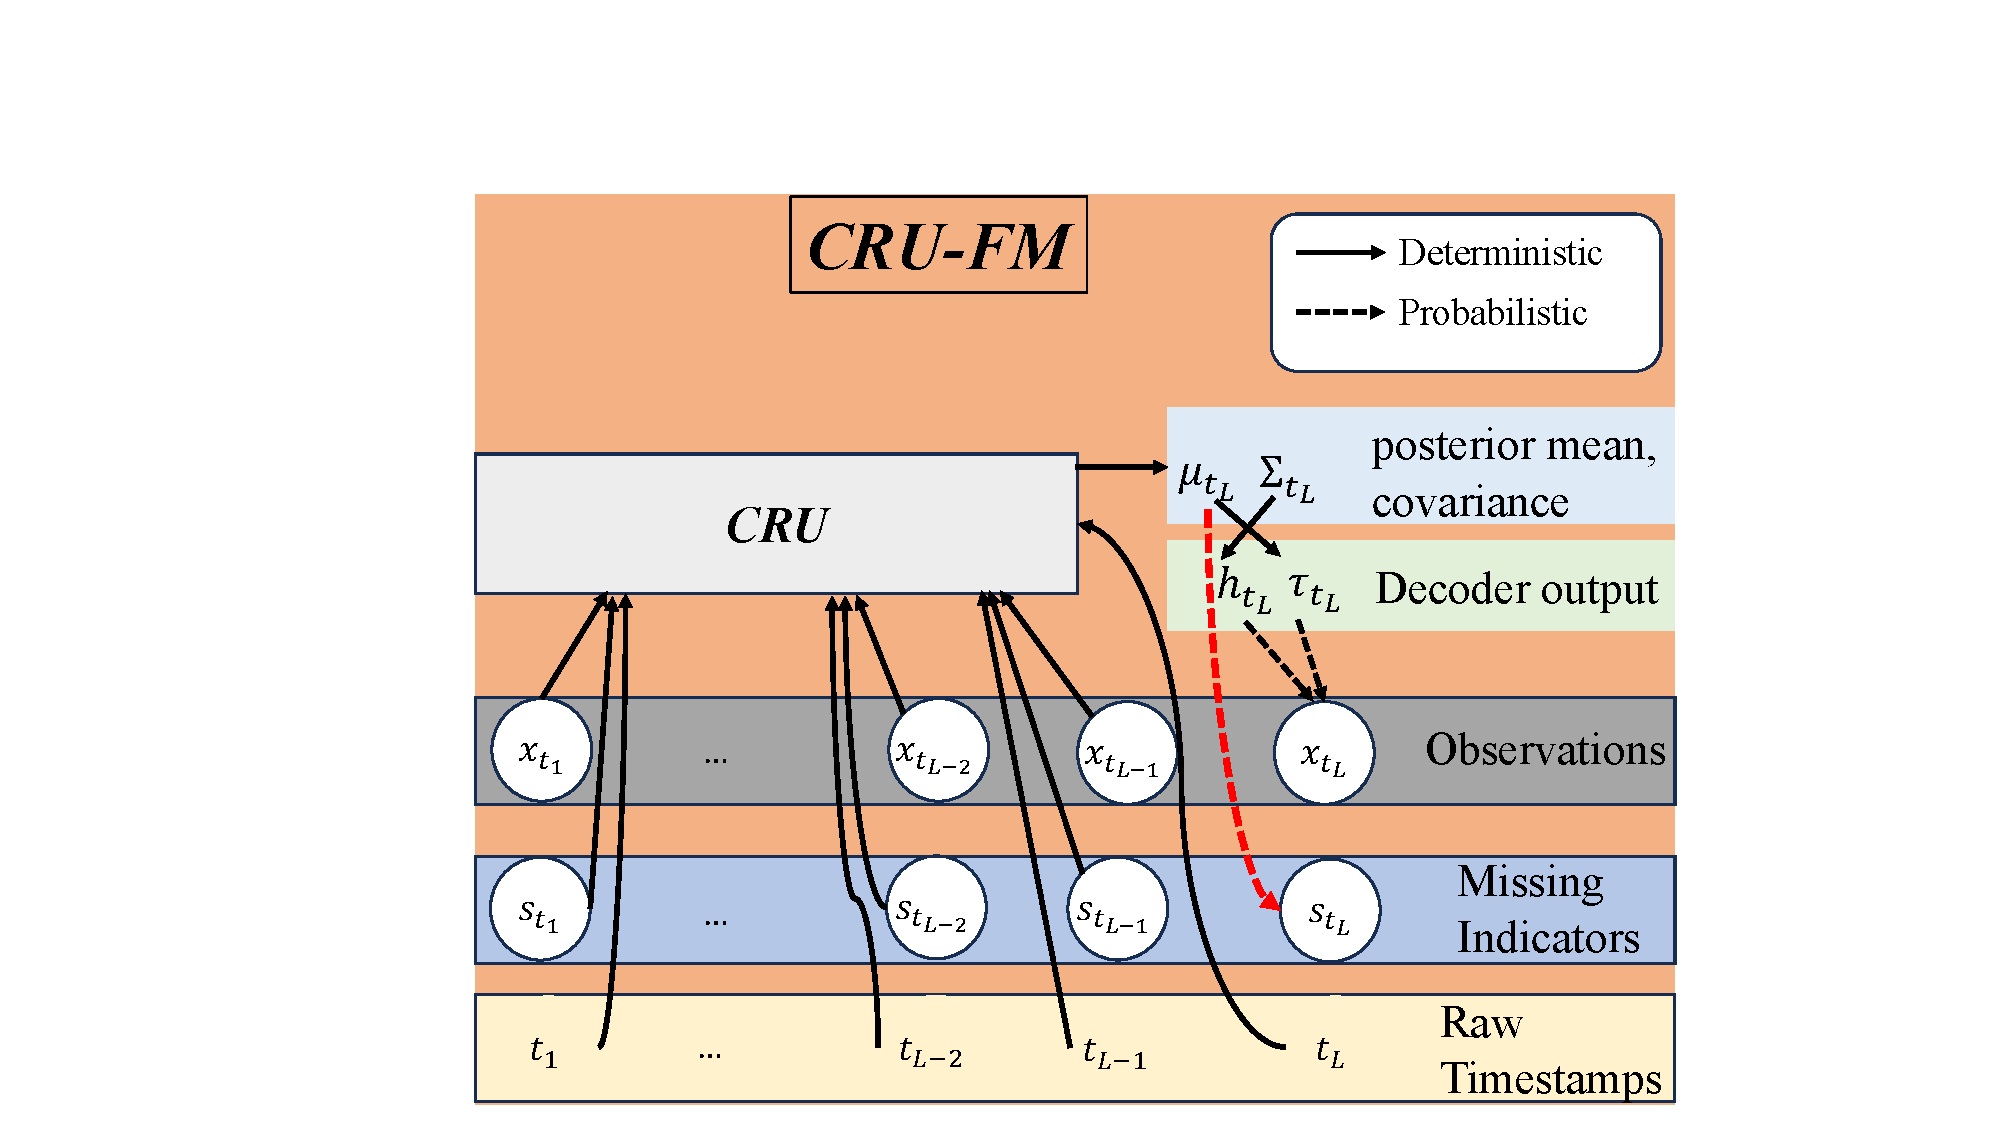
\includegraphics[width=0.9\textwidth]{content/chapters/irregular_time_series_data_driven_missingness/figures/cru_fm_diagram.pdf}
    \caption[Diagram of our proposed CRU-FM model]{Diagram of our CRU-FM model (Sec.~\ref{sec:CRU_gen_model}). We show the extrapolation generative process for data vector $x_{t_L}$ and binary seen/missing indicator $s_{t_L}$ at time $t_L$, conditioning on previous $x_{t_1:t_{L-1}}, s_{t_1:t_{L-1}}$.
    The red line highlights our contribution: a distribution on $s_{t_L}$ that is data-dependent and thus suitable for MAR settings. Dashed lines point to values that are sampled from a distribution, not deterministically computed from predecessors. 
    }%endcaption
    \label{fig:generative_model}
    % \vspace{-.7cm} %% HACK
\end{figure}

\newcommand{\xseen}{x^{\text{S}}}
\newcommand{\xfillzero}{\bar{x}}

\section{Methods}
In order to develop probabilistic models for irregular time series with arbitrary missingness, let us define some essential notation. First, for a given time $t$, let $\xseen_t$ denote the subset of all entries of $x_{t} \in \mathbb{R}^D$ that are \emph{seen} or present, not missing. $\xseen_t$ may vary in size depending on how many entries are missing at time $t$.  Second, let $\bar{x}_{t}$ be a vector of size $D$ constructed from $x_t$ by filling any missing entry with a numerical zero, but otherwise leaving present entries alone. Recalling that $s_t$ is a binary vector indicating the seen entries of $x_t$, we can write $\xfillzero_t \gets x_{t} \odot s_{t}$ to represent the element-wise product (denoted $\odot$) which fills any missing entry with zero.


\subsection{CRU model for seen features only}
\label{sec:CRU_gen_model_from_prev_work}

\citet{schirmer2022modeling} provide the following generative model for $\mathbf{\xseen}$, the \emph{seen} (non-missing) entries of the $D$-dimensional time series $\mathbf{x}$:
\begin{align}
    p( \mathbf{\xseen} ) &= \prod_{t \in \Gamma} p( \xseen_t | \{  \xseen_u : u < t, u \in \Gamma \} ),
    \\ \notag 
    &= \prod_{t \in \Gamma} \prod_{d : s_{td}=1} \mathcal{N}( x_{td} \mid h_{td}, \tau_{td}^2 ),
\end{align}
where $h_t, \tau_t$ are the decoded data representations for time $t$ produced by a CRU given zero-filled input:  $[h_{t_1}, \ldots], [\tau_{t_1}, \ldots] \gets \textsc{CRU}( \bar{x}_{t_1}, \ldots \bar{x}_{t_L}, \Gamma )$. Symbol $\mathcal{N}$ is the Gaussian pdf.

While this model can be fit on irregular time series with arbitrary missingness, we stress that it does not model the missingness indicator $s_t$ as a random variable and thus cannot account for data-dependent missingness mechanisms. Our later experiments show that in both synthetic  and real-world missingness scenarios, this leads to poor recovery of the underlying model and high error in extrapolation.

\subsection{CRU-FM generative model}
\label{sec:CRU_gen_model}
To better capture data-dependent missingness, we propose a generative model of both 
seen features $\mathbf{\xseen}$ and binary seen/missing indicators $\mathbf{s}$ over time. We call this the CRU-FM, emphasizing the joint modeling of both Features and Missingness, and illustrate this model in Fig.~\ref{fig:generative_model}.
The joint distribution is defined as:
%suggest that the generative model fit to data needs to deliberately model both the 
%We call the following our MNAR-CRU model:
\begin{align}
   \label{eq:mnar_cru_model}
   p(\mathbf{\xseen}, \mathbf{s}) 
   &= 
        \prod_{t \in \Gamma}
            p( \xseen_t, s_t | \{  \xseen_u, s_u : u < t, u \in \Gamma \} )
    \\ \notag 
   &=
   \prod_{t \in \Gamma} \left[ 
        \prod_{d : s_{td}=1}
        \mathcal{N}( x_{td} | h_{td}, \tau_{td}^2 )
        \cdot 
        \prod_{d=1}^D
        \text{Bern}( s_{td} | \text{r}(\eta_d^T \mu_t^+) )
        \right]
\end{align}
Here, we again provide zero-filled features $\mathbf{\bar{x}}$ as input to the CRU to obtain the representations: $[h_{t_1}, \ldots], [\tau_{t_1}, \ldots], [\mu^+_{t_1}, \ldots] \gets \textsc{CRU}( \bar{x}_{t_1}, \ldots \bar{x}_{t_L}, \Gamma )$. Note that latent mean $\mu_t^+$ can easily be accessed from step 3 of the CRU algorithm defined in Eq.~\ref{eq:CRU_algorithm}.
For each data dimension $d$, vector $\eta_d \in \mathbb{R}^M$ represents learnable weights for a regression that estimates the probability of observing variable $d$ given the $M$-length vector $\mu^+_t$ from the CRU. Symbol $\text{r}(\cdot)$ denotes the logistic sigmoid function, which maps a real value to a probability in [0,1].

The chosen form of Eq.~\eqref{eq:mnar_cru_model} balances two desiderata. First, we want the generative process for indicator vector $s_t$ to be data-dependent to address MAR scenarios. 
Second, we want to maintain the efficient computational properties of the CRU. Our construction ensures both. The joint over $s_t$ and $x_t$ is clearly dependent on all previous observations $x^S_{1:t-1}$.
However, we can still benefit from the CRU's efficient algorithm in Eq.~\eqref{eq:CRU_algorithm}.


\textbf{Extension.}
A more general extension of our proposed CRU-FM is easily possible, which keeps the same model for $\xseen$ but models each entry of $s_t$ via
\begin{align}
    s_{td} \sim \text{Bern}( r(\eta_d^T \rho(\mu^+_t, h_t, \tau_t, t) )),
    \label{eq:extended_mnar_cru_model}
\end{align}
where function $\rho$ produces a fixed-size vector represention via any deterministic and differentiable mapping of provided representations at time $t$, with a weight vector $\eta_d$ of suitable size. For example, in a hospital care setting, allowing non-linear dependent on the time of day via timestamp $t$ could
%we could allow the probability that feature $d$ is present to depend on the time of day via a nonlinear transformation of the timestamp $t$, to 
capture the fact that typically fewer lab tests are done at night while patients sleep. One example of such a formulation could be : 
\begin{align}
    s_{td} \sim \text{Bern}(r(\eta_{d1}^T\mu_t^+ + \eta_2^Tt)),
    \label{eq:extended_mnar_cru_model_example}
\end{align}
where $\eta_d=\{\eta_{d1}, \eta_{2}\}$
Similarly, by providing decoded data vector $h_t \in \mathbb{R}^D$ and uncertainty $\tau_t \in \mathbb{R}_{+}^D$ as input, the mean and variance values of specific measurements related to feature $d$ could modulate its missingness.  Training this extended CRU-FM would be straightforward. % as described below.

Our later experiments examine only the simpler model in Eq.~\eqref{eq:mnar_cru_model}, so that comparisons directly assess how the addition of data-dependent missingness improves performance.


\subsection{Training}

To train our model, we assume we are given a collection of $N$ irregularly-spaced sequences of the same $D$ possible measurement variables. Each sequence, indexed by $n$, has its own set of observation times $\Gamma_n$, its own seen feature time series $\mathbf{\xseen}_n$, and its own binary indicator vector time series $\mathbf{s}_n$. We assume each sequence is independent and identically-distributed according to the CRU-FM model in Eq.~\eqref{eq:mnar_cru_model}.

We thus frame the goal of fitting the CRU-FM model to $N$ patient records as finding the CRU parameters $\theta$ (defined in Sec.~\ref{sec:CRU}, encompassing the SDE parameters as well as encoder and decoder weights) and data-dependent regression weight $\eta$ (defined in Eq.~\eqref{eq:mnar_cru_model}) that maximize the log likelihood of all $N$ observed sequences under our chosen model. Equivalently, we solve the following optimization problem
\begin{align}
    \theta^*, \eta^* \gets \arg\!\min_{\theta, \eta} 
    ~\lambda \eta^T \eta
    - \sum_{n=1}^N \log p_{\theta, \eta}( \xseen_n, s_n )
\end{align}
where scalar hyperparameter $\lambda > 0$ governs the strength of regularization on regression weights $\eta$ that govern the data-dependent generation of each $s_t$.
Recall that our model's density function $p_{\theta, \eta}(\mathbf{\xseen}_n, \mathbf{s}_n)$ is defined in Eq.~\eqref{eq:mnar_cru_model}. The notation $p_{\theta, \eta}$ reminds us to view this density as a function of parameters $\theta, \eta$. Evaluation of this log likelihood objective and its gradients with respect to $\theta, \eta$ is straightforward using modern automatic differentiation.



%We assume each sequence $x_\tau$, with observation indicator, $s_\tau$ is being mapped to a target sequence $o_\tau$. The training objective is to minimize the loss 
%\begin{align}
%    \mathcal{L}(o_\tau)=\sum_{t \in \tau}\mathcal{N}(o_t|h_t, \tau_t) + \sum_{t \in \tau}\log\text{Bern}(s_t|\sigma(\eta^T \mu_t^+cv b))
%\end{align}
%where $h_t$ and $\tau_t$ are the outputs from the CRU at time time $t$ and $\eta$ are learned weights. 

\subsection{Implementation Details}

We solve parameter estimation using the Adam optimizer \citep{kingma2014adam} training for 100 epochs. We perform hyperparameter search across 2 different batch sizes (64 and 128), 3 different learning rates (0.001, 0.005, and 0.01), and 6 possible regularization strengths $\lambda$ (between $10^{-6}$ and $0.1$) and the choose the configuration with lowest RMSE on the validation set. Details for reproducibility are in the Supplement. For all experiments involving both the basic zero-fill CRU model as well as our CRU-FM model, we use the efficient implementation of CRU proposed by \cite{schirmer2022modeling} as \emph{f-CRU}. This method simplifies the dynamics of $z(t)$ by representing matrix A as a weighted average of K basis matrices with shared orthogonal eigenvectors, reducing the matrix exponential's complexity from $O(M^3)$ to $O(KM)$ in Eq.~\eqref{eq:LTI_SDE}.

\subsection{Evaluating Extrapolations}
\label{sec:evaluating_extrapolations}
In later experiments, we wish to evaluate how well our model can extrapolate beyond the provided observation times $\Gamma$. For each sequence of interest, we'll suppose we have additional future times of interest $\Gamma^*$ (all larger than the times in $\Gamma$).
%The procedure below makes \emph{predictions} $\hat{x}^*_t$ of future feature values for all $t\in \Gamma^*$, conditioning \emph{only} on the observed $x_t$ for $t \in \Gamma$. 

%may still be truly missing: our evaluations only use the observed ones, satisfying $s^*_{td} = 1$. 

Given parameters $\theta$ defining our CRU-FM model, we make extrapolative \emph{predictions} $\hat{x}^*_t$ of future feature values for all $t\in \Gamma^*$. The procedure is a straightforward sequence of steps, all of which condition \emph{only} on the observed $x_t$ for $t \in \Gamma$.
First, we obtain representations $h_t, \tau_t$ for each $t$ in the union of $\Gamma \cup \Gamma^*$ by running the CRU algorithm forward as in Eq.~\eqref{eq:CRU_algorithm}.
For the observed times in $\Gamma$, the algorithm runs as written.
For the heldout times in $\Gamma^*$, we modify the algorithm to just do forward prediction and decoding. No observation in $x^*$ impacts the extrapolation. We skip step 1, for step 2 we define $t'$ as the last time in $\Gamma$, we skip step 3, and for step 4 we compute $h_t, \tau_t \gets g_{\phi}(\mu^-_t, \Sigma^-_t)$. Ultimately, we predict the most likely feature value at each dimension and time, via
\begin{align}
    \hat{x}^*_{td} \gets h_{td}, \text{for all}~ t \in \Gamma^*, ~d : s^*_{td} {=} 1
\end{align}
%Finally, we can assess error by comparing the estimated value to the (heldout) actual value. 

Across all future times, we then compute and report error between the prediction $\hat{x}^*_t$ and the seen ground-truth features $x^{*\text{S}}_t$, using only dimensions $d$ where we have ground-truth (satisfying $s^*_{td} = 1$) and ignoring the others.

\begin{figure}[!t]
    \centering
    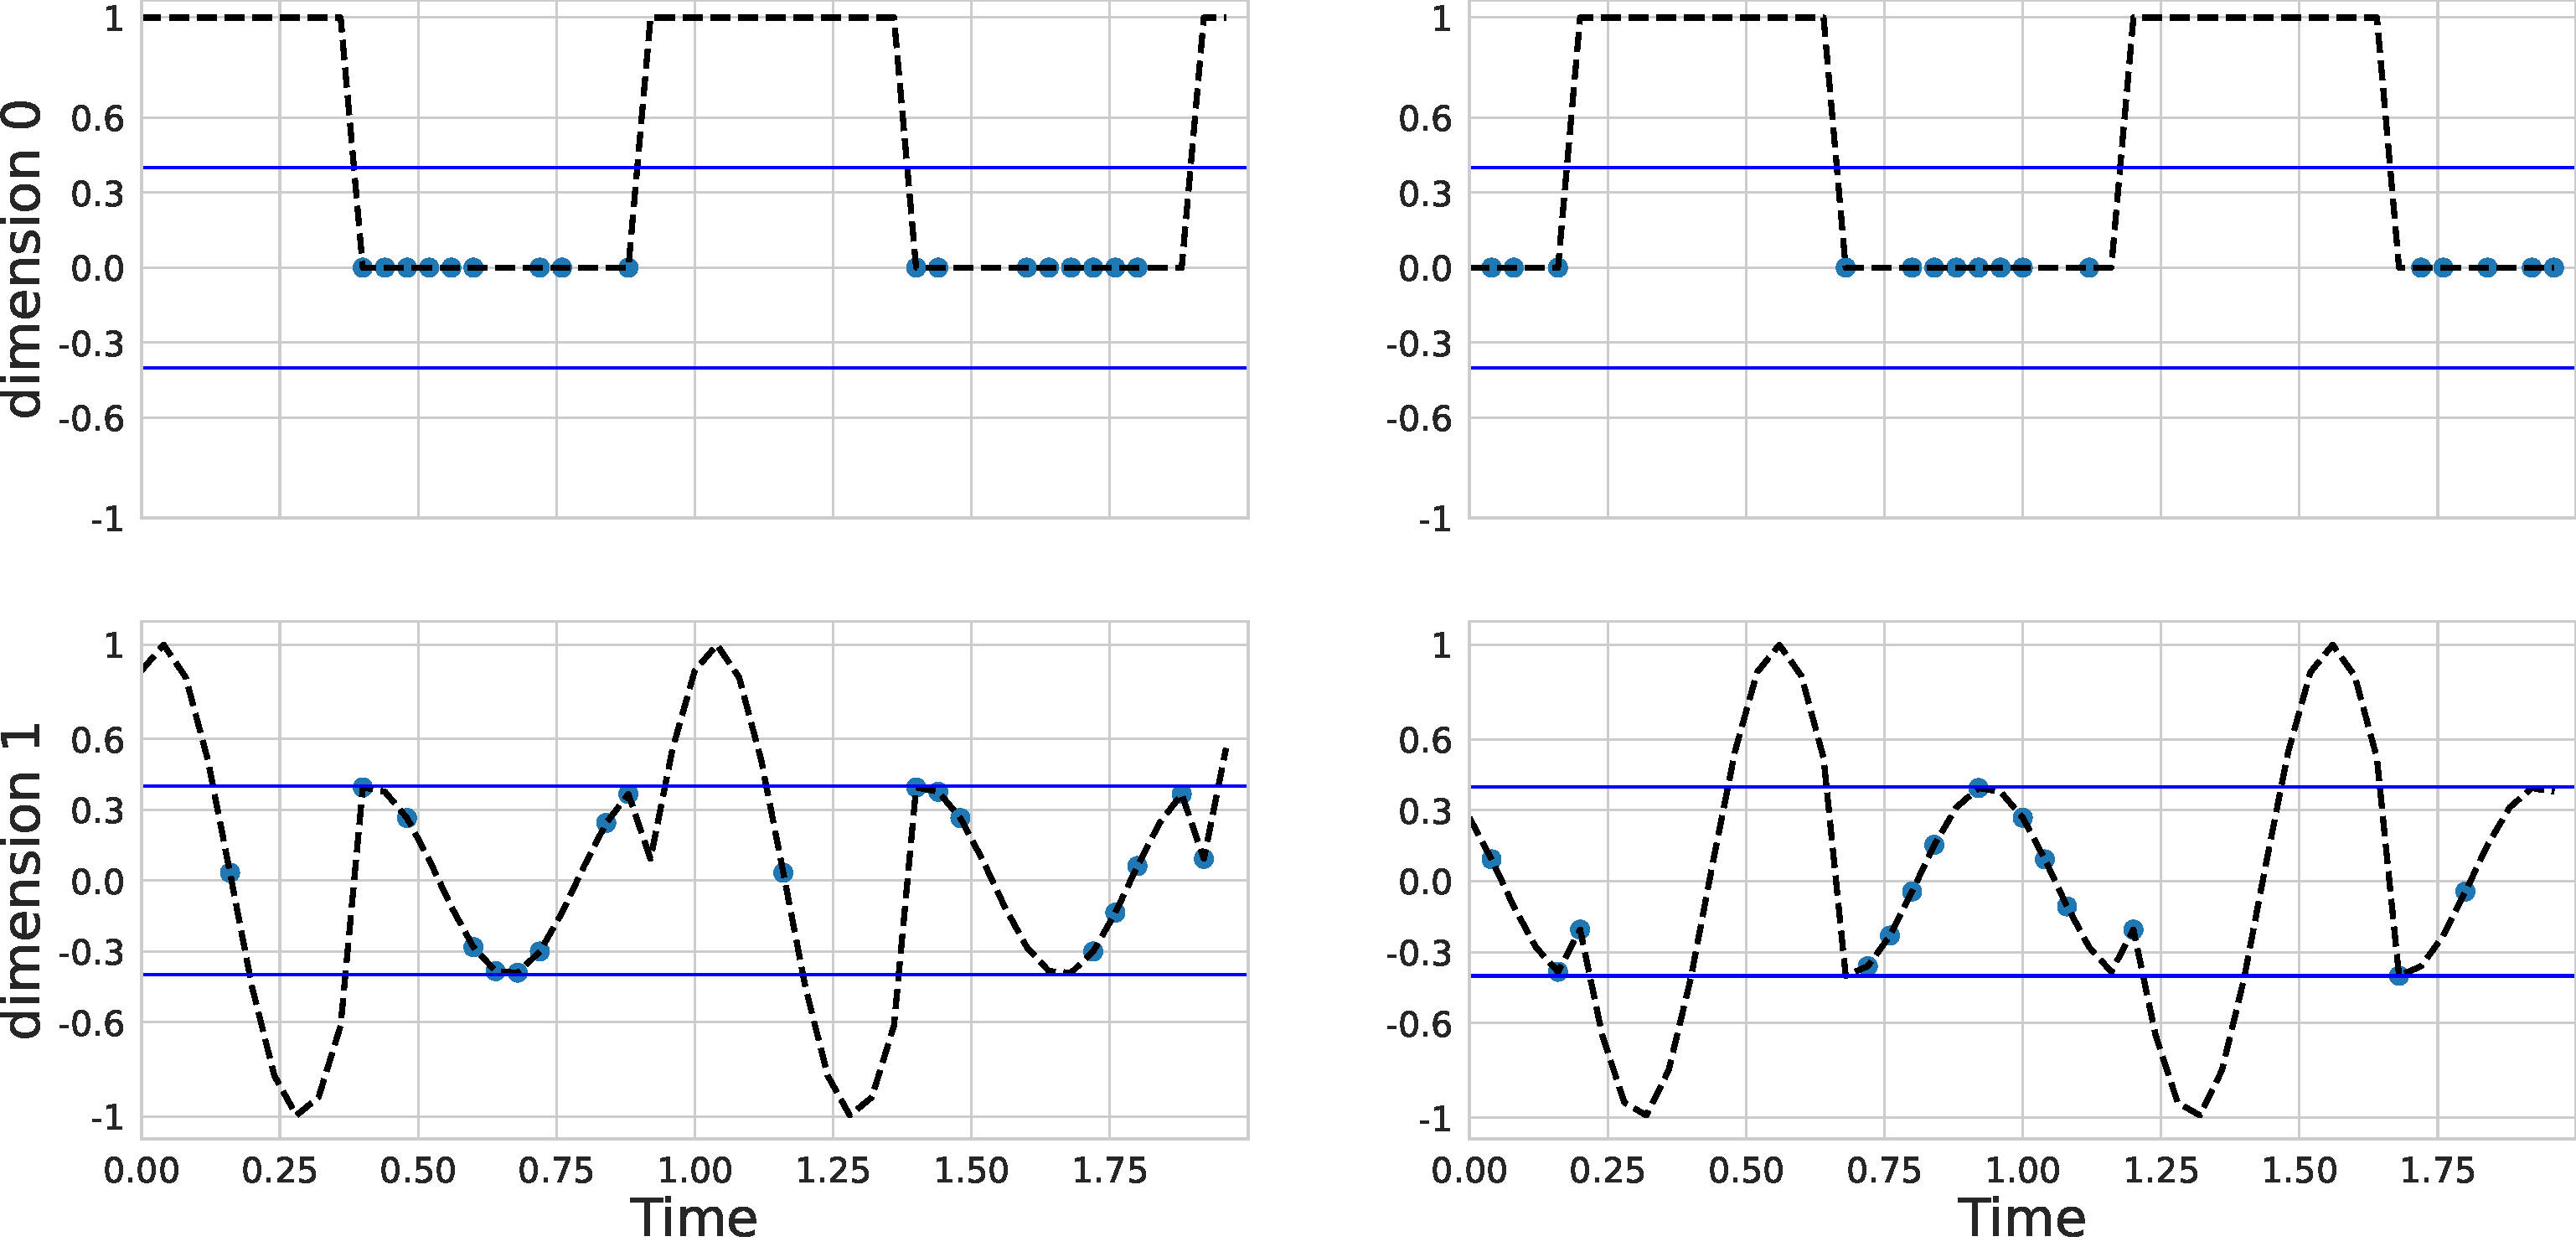
\includegraphics[width=0.9\textwidth]{content/chapters/irregular_time_series_data_driven_missingness/figures/toy_data.pdf}
    \caption[Examples of generated sequences for the synthetic task]{Two examples of generated sequences for the synthetic task. The dashed black lines represent the true data-generating process. The circular dots represent the observations at irregular timepoints. To incorporate data-dependent missingness, the probability of observing a value within the solid blue lines is 0.6; outside the lines is $p_{\text{S}}=0.0006$.}
    \label{fig:toy_example_sequences}
\end{figure}

\section{Experimental Results}
We now assess our CRU-FM model experimentally.
First, we study a synthetic task where we can control the missingness mechanism precisely (varying between data-dependent and data-independent). 
Second, we study extrapolation performance on 3 real open-access datasets of critical care electronic health records (EHR).

%as well as on thre large open-access datasets of critical care electronic health records (EHR): Physionet(specifically the computing in cardiology challenge 2012 \citep{silva2012predicting}) and MIMIC-IV \citep{johnson2020mimic}. 


We compare to 6 total competitive baselines for irregular time series modeling.
First, 
\citet{schirmer2022modeling}'s CRU model (Sec.~\ref{sec:CRU_gen_model_from_prev_work}) is a natural baseline, as it represents removing the data-dependent missingness mechanism of our CRU-FM.
Additionally, we compare to 
 mTAND \citep{shukla2021multitime}, pVAE \citep{li2020learning},
 Latent ODE~\citep{rubanova2019latent}, and Neural CDE~\citep{kidger2020neural}. 
On the synthetic task, we also compare to an additional recent LLM baseline for time series forecasting called LLMTime \citep{gruver2023large}. Due to its poor performance, we did not apply it to any EHRs.
%on this toy task, we did not spend time applying this baseline to later large EHR datasets.


\subsection{Synthetic Experiments}
\label{sec:synthetic_experiment}


\textbf{Purpose.}
We designed a synthetic extrapolation task with $D{=}2$ data channels to assess how well each model can learn from hundreds of sequences drawn from a known data-generating process that includes data-dependent missingness (defined in equations \ref{eq:gen_data_toy_eq} and \ref{eq:seen_proba_toy}).
Figure~\ref{fig:toy_example_sequences} illustrates two example sequences.
The top channel is a square wave with a sequence-specific phase offset.
The bottom channel is a sinusoid whose amplitude and phase depend on the  current value of the top channel.  
As detailed below, our data-generation process introduces missingness in a channel at different rates depending on whether the channel's current value is inside or outside the illustrated blue horizontal bounds. 

This process results in significant missingness in the top (first) channel. Thus, in order to deliver good extrapolations for both channels, a model must accurate model dependencies in feature values and missingness jointly across channels.

\textbf{Setup.}
To generate each sequence (indexed by $n$), we draw a horizontal offset $b_n \sim \text{Unif}([0,2])$. 
This value informs a deterministic ``true'' time-varying data-generation function $x_{n,d}(t)$ for each dimension $d$: we have a square wave for $d=1$ and a sine wave for $d=2$ 
\begin{align}
    x_{n,1}(t) &= \operatorname{sgn}(\sin(4\pi t+b_n))
    \\ \notag 
    x_{n,2}(t) &= \sin(4\pi t+b_n) \cdot x_{n,1}(t)
    + 0.4 \cdot \cos(4\pi t+b_n) \cdot (1-x_{n,1}(t))
\label{eq:gen_data_toy_eq}
\end{align}

For each sequence $n$, a set $\Gamma_n$ of observation times is drawn with 50 elements, each one i.i.d. uniform within $(0, 2)$. At each time $t \in \Gamma_n$, the indicator controlling whether dimension $d$ is seen or missing is then sampled so that inside the blue lines of Fig.~\ref{fig:toy_example_sequences}, there is a good chance of observation (60\%), but outside the lines the chance is lower:
\begin{align}
     p( s_{ntd} = 1 ) =
 \begin{cases}
 0.6 & \text{if } -0.4 < x_{n,d}(t) < 0.4 \\
 p_{\text{S}} & \text{otherwise }
 \end{cases}    
 \label{eq:seen_proba_toy}
\end{align}
Here, scalar $p_{\text{S}} {>} 0$ determines the chance of seeing an outside-the-lines value. By default, we fix $p_{\text{S}} {=} 0.0006$, yielding a data-dependent missingness mechanism for both channels. 
Later sensitivity analyses study what happens as $p_{\text{S}}$ increases toward 0.6 (MCAR scenario).


\textbf{Extrapolation task.}
We generated 1000 sequences (keeping only the $x_{nt}, s_{nt}$ values at times in $\Gamma_n$), divided into train/valid/test splits of size 700/150/150. 
After training and tuning any model, we measure extrapolation on each test sequence by providing data up to time $t=1.5$, then obtaining from each model the \emph{most likely} predicted value for each channel at each heldout time in $(1.5, 2.0)$.



%  The MNAR conidtion is as follows : 
% \[
% p(s_{n,k}(t)=1|f_{n,k}(t)) =
% \begin{cases}
% 0.6 & \text{if } -0.4 < f_{n,k}(t) < 0.4 \\
% 0.0006 & \text{otherwise }
% \end{cases}
% \]
% where $s_{n,k}(t)$ is an indicator for observing data in the $k^{th}$ channel of the $n^{th}$ sequence at time $t$. $s=1$ if data is observed and 0 otherwise. 2 example sequences are shown in figure \ref{fig:toy_example_sequences}. We generate 800 sequences and divide the train/valid/test splits as 500/150/150. We choose the best model as the one with the lowest validation mean-squared-error in the extrapolated segment (highlighted by dashed lines at $t>1.5$ in figure \ref{fig:models_generated_seq}).



\begin{figure*}[!ht]
\centering
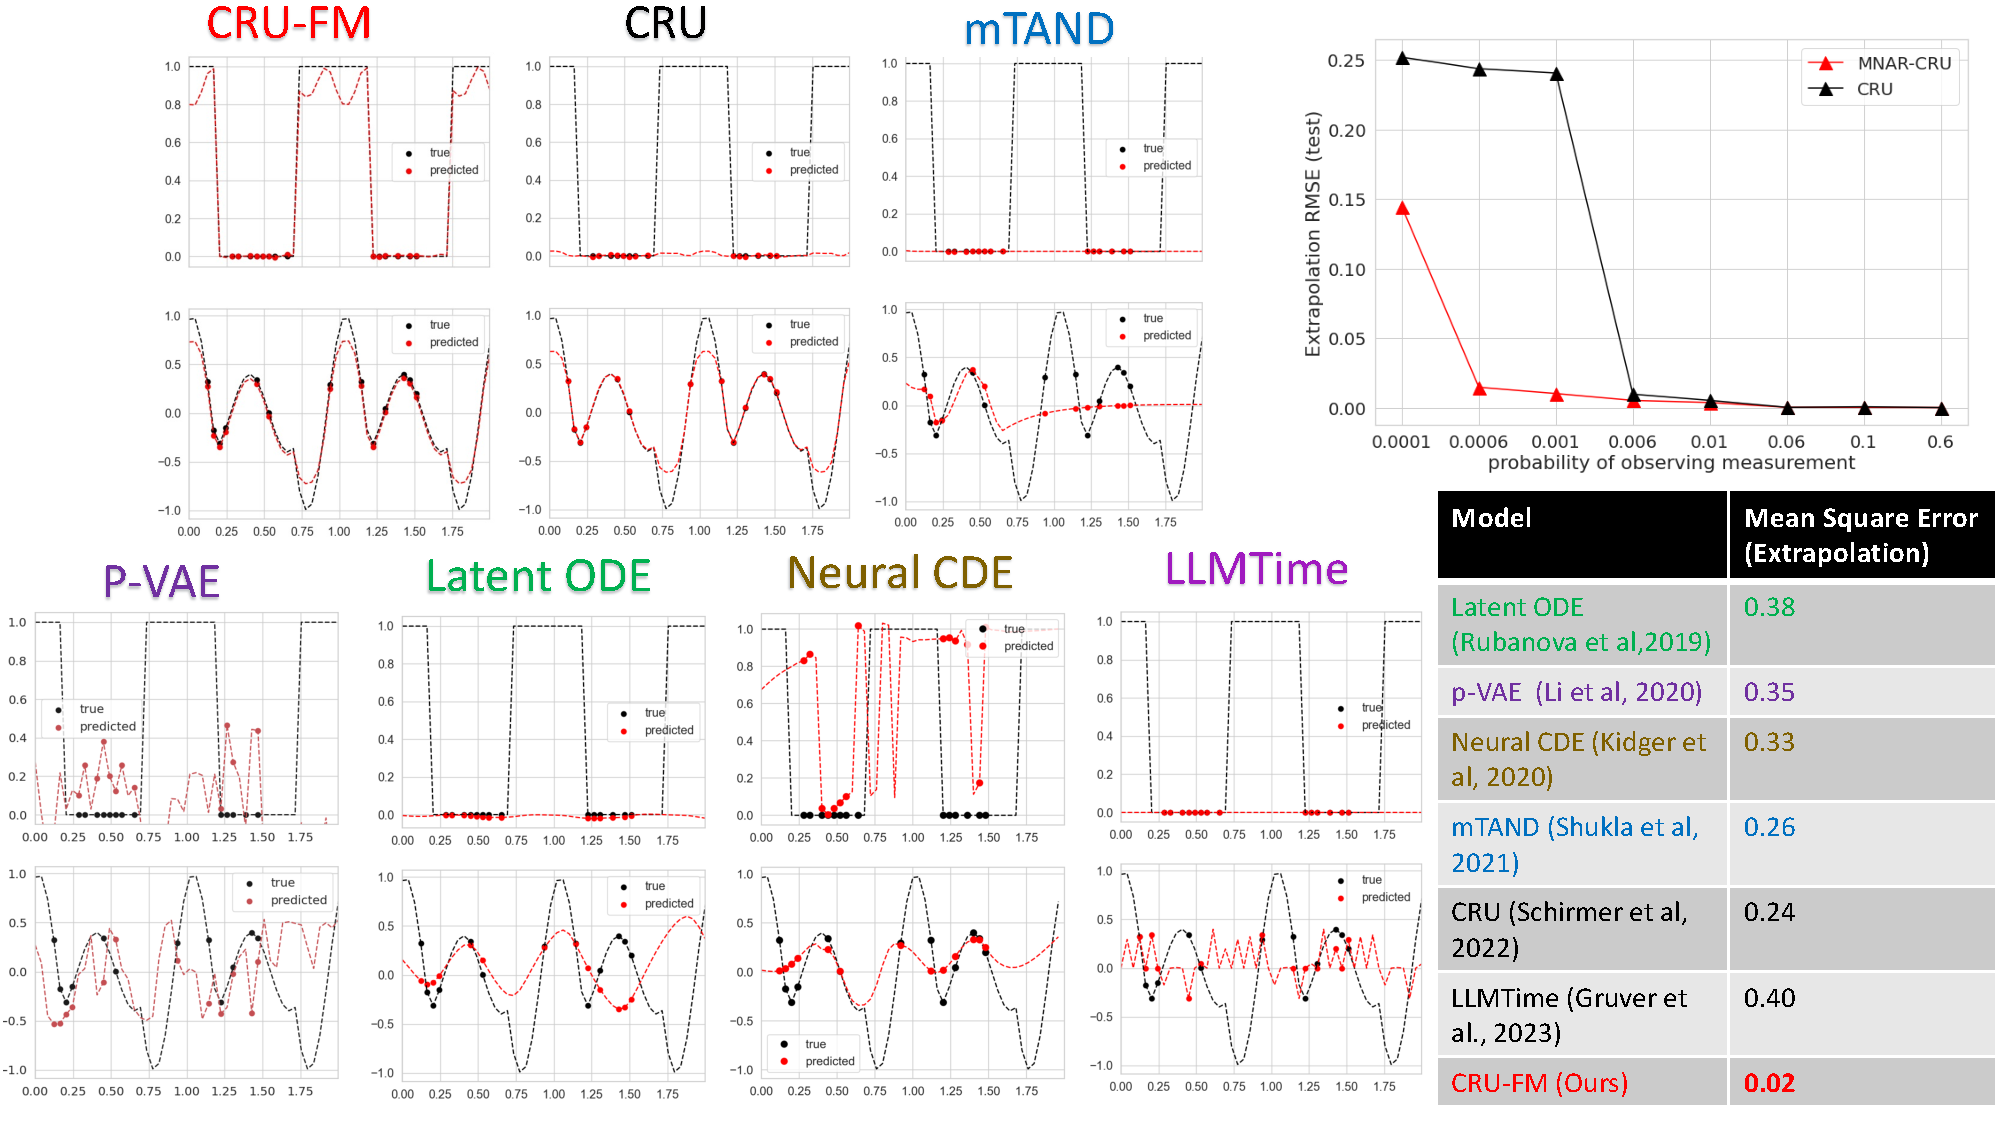
\includegraphics[width=1.0\textwidth]{content/chapters/irregular_time_series_data_driven_missingness/figures/toydata_extrapolation_improved.pdf}
\caption[Synthetic task results comparing CRU-FM to competitors]{Synthetic task results comparing CRU-FM to competitors.
\emph{Left:} Visuals of reconstruction ($t \in (0, 1.5)$) and extrapolation ($t \in (1.5, 2)$) for the \emph{same} 2-channel test sequence when missingness is data-dependent ($p_{\text{S}} {=} 0.0006$).
Black (red) lines indicate true (reconstructed) values. To fairly compare models, we evaluate each one's most likely prediction $\hat{x}_{t}$ (mode of the predictive distribution). 
For example, for our CRU-FM we set $\hat{x}_{t} = h_{t}$ (via Eq.~\eqref{eq:mnar_cru_model}).
This choice eliminates extraneous randomness needed to sample from a predictive distribution.  \emph{Bottom Right:}
Extrapolation results on the synthetic task sequences comparing MNAR-CRU, CRU, MTAND and p-VAE. The black/red dots are the observed/predicted values at each irregularly sampled time point. The black/red line is the true/reconstructed sequence. Each model is trained until $t=1.5$ and the extrapolated from $t=1.5$ to $t=2$. MNAR-CRU generates sequences that are closer to the ground-truth and also achieves the least mean squared error on the extrapolation task. We attribute this improved performance of the MNAR-CRU to the model's ability to learn the true missingness probability in each sequence. \textit{Top right :} We examine how extrapolation error changes as the probability of observing a measurement (denoted as $p_{obs}$) outside the (-0.4, 0.4) bounds changes. As $p_{obs}$ increases (MNAR assumption relaxes), as expected the CRU and MNAR-CRU perform similarly. For low values $p_{obs} \leq 0.006$, MNAR-CRU’s better-specified missingness model notably improves extrapolation (via a joint model of $x_t$ and $s_t$).
}%endcaption
\label{fig:models_generated_seq}
\end{figure*}

\textbf{Results: Head-to-head comparison with competitor models :}
Fixing $p_{\text{S}} = 0.0006$ to ensure data-dependent missingness, we compare the extrapolation error of our CRU-FM with all competitors.
In the lower right panel of Fig.~\ref{fig:models_generated_seq},
CRU-FM delivers by far the lowest overall mean squared error on the test set of 150 sequences (0.02 vs. 0.24 for the next best competitor, the CRU). 

To understand possible reasons for CRU-FM's improved performance, we show plots of sequence-specific reconstructions/extrapolations from each model 
(left panels of Fig.~\ref{fig:models_generated_seq}).
These plots confirm CRU-FM recovers the underlying ``true'' model structure best, especially looking at the more difficult first (top) channel.
All models are trained on the same 700 sequences, few of which do have rare cases of observations from the top of the square wave. 
We suggest our model handles this top channel better than alternatives because it is the only tested model capable of data-dependent missingness. 
CRU-FM's
 latent representations $\mu_t$ are informed by both features $x_t$ and seen/missing indicators $s_t$, enabling learning of dependencies between channels (e.g. steep slope in channel 2 is indicative of a crest in channel 1 even when channel 1 is often missing). 
%ltimately resulting in superior extrapolative performance.

%It's important to note that data points are not $100\%$ missing at the crest of the square-wave but have a very low probability of observation: 0.0006. Given that our training involves 700 sequences drawn from the same process (see Fig 2 and the equation below it), the model does encounter a number of sequences that include observations in the crest/peak of the square wave. Thanks to our joint model, the variables \(x_t\) and \(s_t\) are informed by posterior means (\(\mu_t^+\)), enabling learning of dependencies between channels (e.g. steep slope in channel 2 is indicative of a crest in channel 1, ultimately resulting in superior extrapolative performance.

As illustrated in Fig.~\ref{fig:models_generated_seq}, 
the second (bottom) channel is extrapolated similarly well by both the CRU and the CRU-FM, both much better than other models.
We suggest two possible reasons CRU is similar to CRU-FM on this channel.
First, channel 2 spends less time outside the (-0.4, 0.4) bounds and is thus typically observed.
Second, unlike the sharp jump of the square wave in channel 1, the true function of channel 2 transitions \textit{smoothly} across the (-0.4, 0.4) bounds, so sane extrapolations are possible even for simpler models.

\textbf{Results: Sensitivity analysis to missingness mechanism.}
To further verify that capturing the data-dependent missingness of our model is the primary reason for success,
we sweep $p_{\text{S}}$ from 0.0006 to 0.6 (MCAR). At each value,
we resample all train/valid/test data and retrain the CRU-FM and CRU. As expected, the top-right panel in Fig.~\ref{fig:models_generated_seq} shows that our CRU-FM yields far lower error in the data-dependent missingness setting, but becomes indistinguishable from the CRU in the MCAR setting. This helps rule out other confounding explanations for which model is superior, like better tuning or lucky initialization.


\textbf{Results : Parameter Learning on Toy Data}
We show the capability of our model to learn the missingness parameter for each channel in our toy example in figure \ref{fig:learning_missingness_mechanism}
\begin{figure}[h]
    \centering
    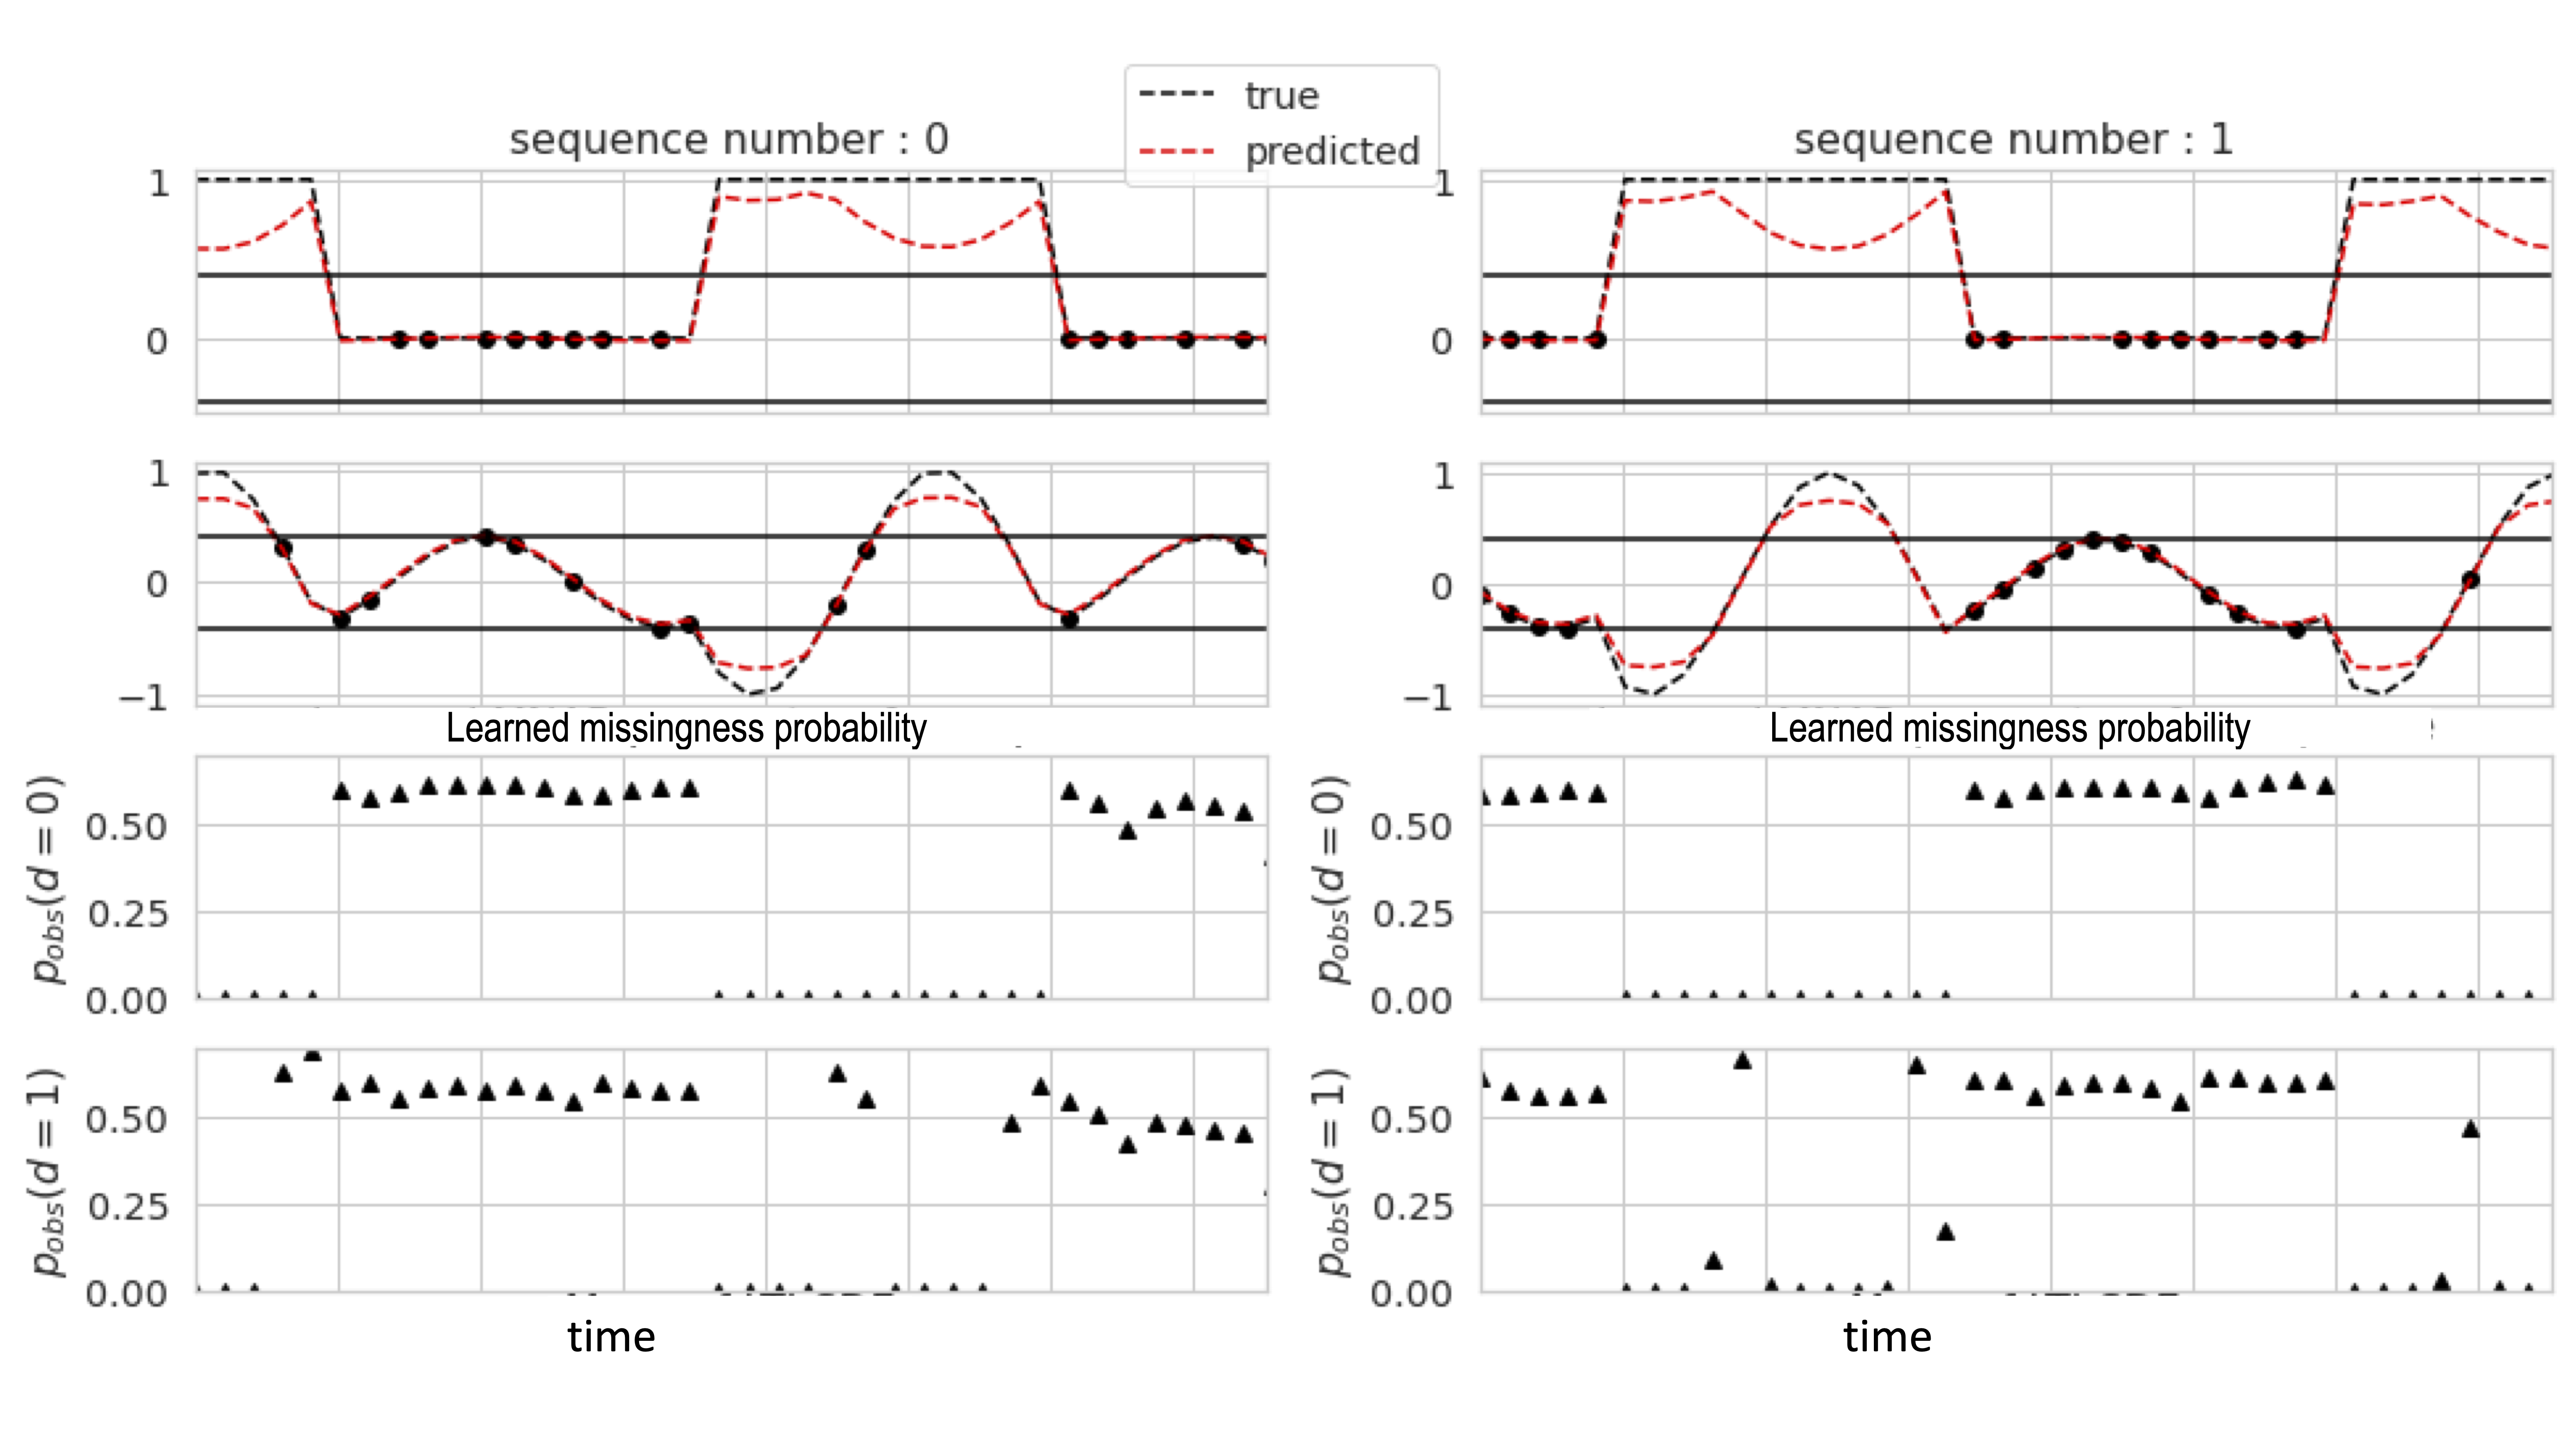
\includegraphics[width=1.0\textwidth]{content/chapters/irregular_time_series_data_driven_missingness/figures/learning_mnar_mechanism.png}
    \caption[Demonstration of our CRU-FM model’s ability to learn the data-dependent missingness mechanism]{Demonstration of our CRU-FM model's ability to learn the data-dependent missingness mechanism. \textit{Top 2 rows : } We show the 2 channels of data from 2 representative sequences from our toy experiment (details in section \ref{sec:synthetic_experiment}). The black dashed line and the red dashed line represent the true and reconstructed sequences respectively. The black dots represent the observed values at irregularly spaced timepoints. \textit{Bottom 2 rows : } Learned probabilities of observing a measurement in each of the channels above.
    Remember, we set the data-dependent missingness mechanism as follows : the probability of observing a value outside the dashed black lines for each channel is 0.0006 and the probability of observing a measurement within the dashed black lines is 0.6. This mechanism is learned by our model (the black upward arrows show the learned probabilities of observing a value). The ability of our model to learn these data-dependent missingness mechanisms leads to improved downstream extrapolation performance.}
    \label{fig:learning_missingness_mechanism}
\end{figure}


\subsection{Results on Real EHR Datasets}
Next, we examine extrapolation error when trained models from different competitor methods get to observe the first 24 hours of patient health-records (labs and vitals) then must extrapolate the same measurements over the next 6-24 hours. We evaluate on 3 separate large EHR datasets that are all de-identified and publicly available.

\textbf{Physionet-2012 setup.} 
The Physionet-2012 challenge dataset \citep{silva2012predicting} is available at \href{https://physionet.org/content/challenge-2012/1.0.0/.}{https://physionet.org/content/challenge-2012/1.0.0/}. 
%contains 8000 ICU stays.
We only include 8000 ICU stays lasting at-least 48 hours and exclude static measurements, following earlier analyses by \citet{rubanova2019latent}.
For each stay, we model all 37 labs and vitals available in released data (see Tab.~\ref{tab:physionet_features} for feature details and missingness rates).
Our train/valid/test splits have 4800/1600/1600 patient stays.
\begin{table}[!ht]
    \centering
    \begin{tabular}{|c|c|c|c|} \hline 
         Feature&  Min&  Max& Observation rate per hour  (averaged over first 48 hours)\\ \hline 
         Weight&  0.0&  300& 0.640\\ \hline 
         Albumin&  0.00&  4.70& 0.012\\ \hline 
         ALP&  0&  1024& 0.016\\ \hline 
         ALT&  0&  11030& 0.016\\ \hline 
         AST&  0&  16200& 0.016\\ \hline 
         Bilirubin &  0&  45.8& 0.016\\ \hline 
         BUN&  0&  170& 0.071\\ \hline 
         Cholesterol&  0&  240& 0.002\\ \hline 
         Creatinine&  0&  16& 0.072\\ \hline 
 DiasABP& 0& 268&0.768\\ \hline 
 FiO2& 0& 1&0.170\\ \hline 
 GCS& 0& 15&0.327\\ \hline 
 Glucose& 0& 1075&0.067\\ \hline 
 HCO3& 0& 42&0.070\\ \hline 
 HCT& 0& 61.8&0.095\\ \hline 
 HR& 0& 211&1.170\\ \hline 
 K& 0& 9.4&0.075\\ \hline 
 Lactate& 0& 31&0.043\\ \hline 
 Mg& 0& 7.7&0.070\\ \hline 
 MAP& 0& 300&0.757\\ \hline 
 Mechvent& 0& 1&0.162\\ \hline 
 Na& 0& 165&0.070\\ \hline 
 NiDiasABP& 0& 161&0.497\\ \hline 
 NIMAP& 0& 165.3&0.493\\ \hline 
 NiSysABP& 0& 296&0.500\\ \hline 
 PaC02& 0& 98&0.122\\ \hline 
 Pa02& 0& 500&0.121\\ \hline 
 pH& 0& 187&0.127\\ \hline 
 platelets& 0& 1047&0.074\\ \hline 
 RespRate& 0& 95&0.277\\ \hline 
 Sa02& 0& 100&0.041\\ \hline 
 SysABP& 0& 278&0.768\\ \hline 
 Temp& -17.8& 42.2&0.454\\ \hline 
 TroponinI& 0& 46.2&0.002\\ \hline 
 TroponinT& 0& 24.9&0.010\\ \hline 
 Urine& 0& 11000&0.713\\ \hline 
 WBC& 0& 528&0.067\\ \hline
    \end{tabular}
    \caption{List of features for Physionet}
    \label{tab:physionet_features}
\end{table}


\textbf{MIMIC-IV setup.} 
 Out of single-hospital MIMIC-IV dataset \citep{johnson2020mimic}, we select 
 43,883 ICU stays that last at least 30 hours.
For each stay, we track 37 time-varying labs and vitals used in prior works \citep{Gong, Nestor} (see Tab.~\ref{tab:mimic_features} for feature missingness details).
Our train/valid/test splits have 28084/7022/8777 patient-stays. 
\begin{table}[!ht]
    \centering
    \begin{tabular}{|c|c|c|c|} \hline 
         Feature&  Min&  Max& Observation rate per hour  (averaged over first 48 hours)\\ \hline 
         CRP&  0.4&  286& 0.0005\\ \hline 
         Bilirubin (direct)&  0.1&  19.7& 0.0015\\ \hline 
         Venous CO2 pressure&  20&  97& 0.008\\ \hline 
         Fibrinogen&  71.39&  792.22& 0.008\\ \hline 
         Glucose (blood)&  68&  313& 0.024\\ \hline 
         pH (venous)&  7.09&  7.53& 0.011\\ \hline 
         Height&  135&  193& 0.012\\ \hline 
         Albumin&  1.7&  4.5& 0.008\\ \hline 
         TroponinT&  0.01&  10.40& 0.011\\ \hline 
 Resp rate& 8& 35&0.014\\ \hline 
 Pa02& 51& 478&0.037\\ \hline 
 PaC02& 22& 78&0.037\\ \hline 
 pH (Arterial)& 7.09& 7.53&0.039\\ \hline 
 Bilirubin (total)& 0.2& 25.28&0.016\\ \hline 
 AST& 10& 6958.04&0.016\\ \hline 
 ALT& 5& 5200&0.016\\ \hline 
 Weight& 43.4& 158.9&0.014\\ \hline 
 Lactic acid& 0.6& 15&0.033\\ \hline 
 PT& 10.2& 52.7&0.043\\ \hline 
 Calcium& 6.5& 10.4&0.056\\ \hline 
 Phosphorus& 1.2& 9.0&0.056\\ \hline 
 Magnesium& 1.3& 3.2&0.060\\ \hline 
 ABP (systolic)& 78& 178&0.700\\ \hline 
 ABP (diastolic)& 34& 110&0.700\\ \hline 
 Temperature& 35.4& 38.6&0.220\\ \hline 
 Glucose (serum)& 63& 399&0.061\\ \hline 
 Platelets& 23& 570&0.060\\ \hline 
 Hemoglobin& 6.3& 15.2&0.070\\ \hline 
 Creatinine& 0.4& 8.7&0.060\\ \hline 
 Hematocrit& 19.4& 45.2&0.070\\ \hline 
 Potassium& 2.9& 6.4&0.070\\ \hline 
 HCO3& 10& 37&0.060\\ \hline 
 Chloride& 85& 121&0.070\\ \hline 
 Sodium& 120& 154&0.070\\ \hline 
 Resp Rate& 8& 35&0.950\\ \hline 
 O2 sat& 88& 100&0.940\\ \hline 
 Heart rate& 49& 133&0.960\\ \hline
    \end{tabular}
    \caption{List of features for MIMIC-IV}
    \label{tab:mimic_features}
\end{table}


\begin{figure}[!hp]
    \centering
    \begin{tabular}{l c c c}
        \rotatebox{90}{\hspace{3em}MIMIC-IV} 
        &
        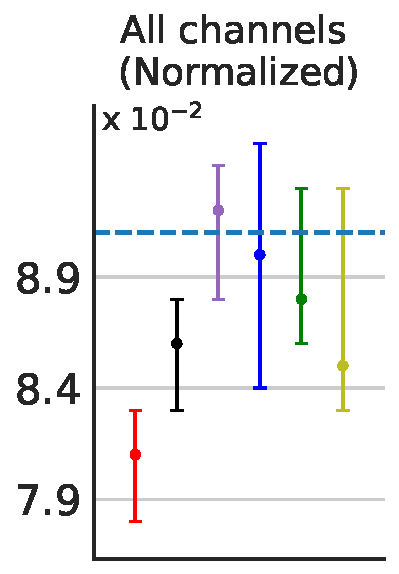
\includegraphics[height=5.2cm]{content/chapters/irregular_time_series_data_driven_missingness/figures/mimic_evaluation_summary.pdf} 
        &
        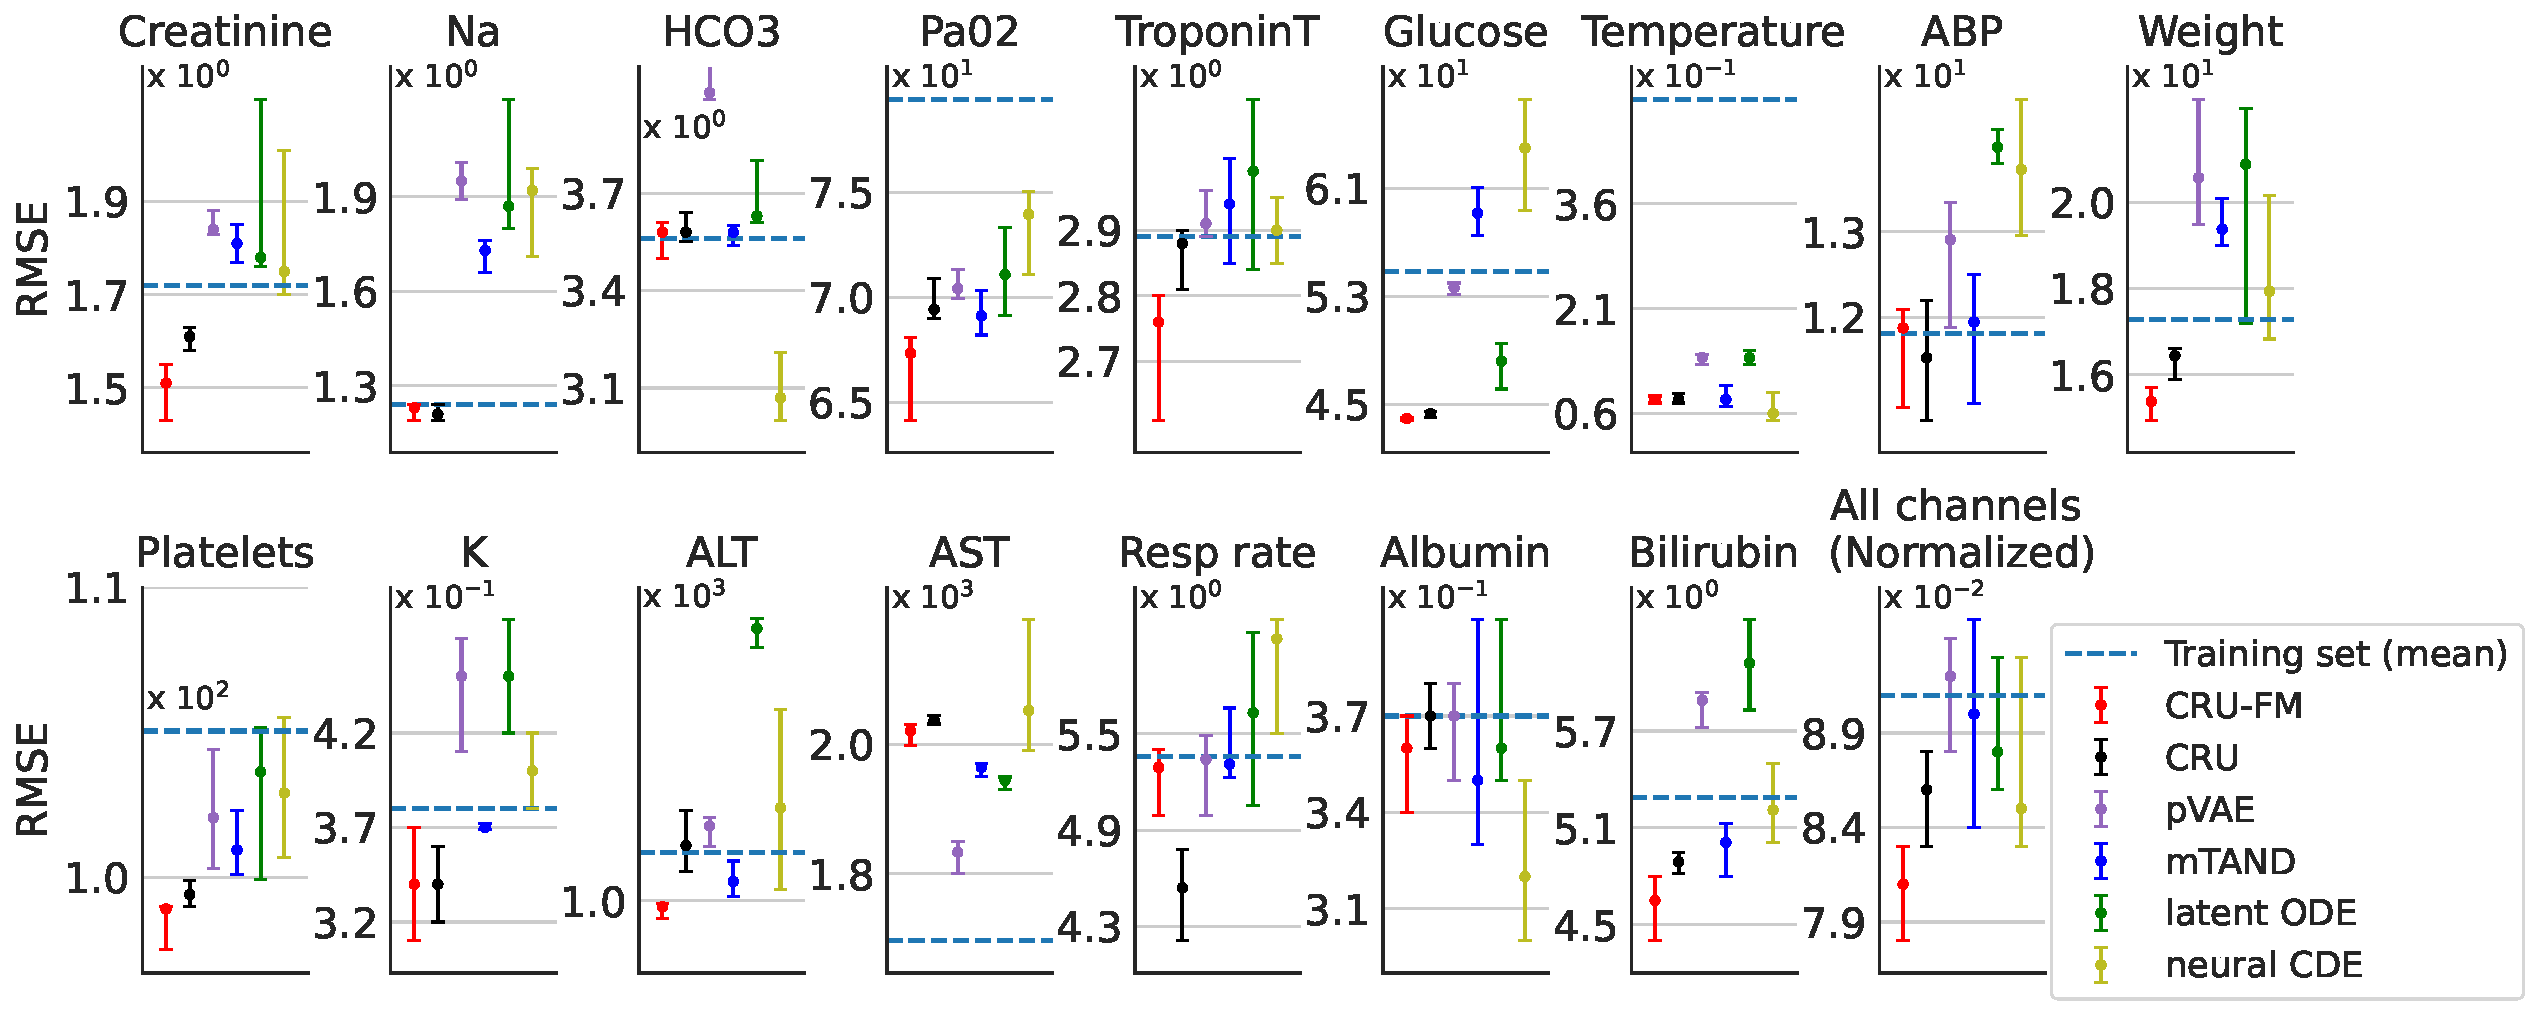
\includegraphics[trim={0 0 590 0},clip,height=5.2cm]{content/chapters/irregular_time_series_data_driven_missingness/figures/mimic_evaluation.pdf} 
        &
        \raisebox{1.5cm}{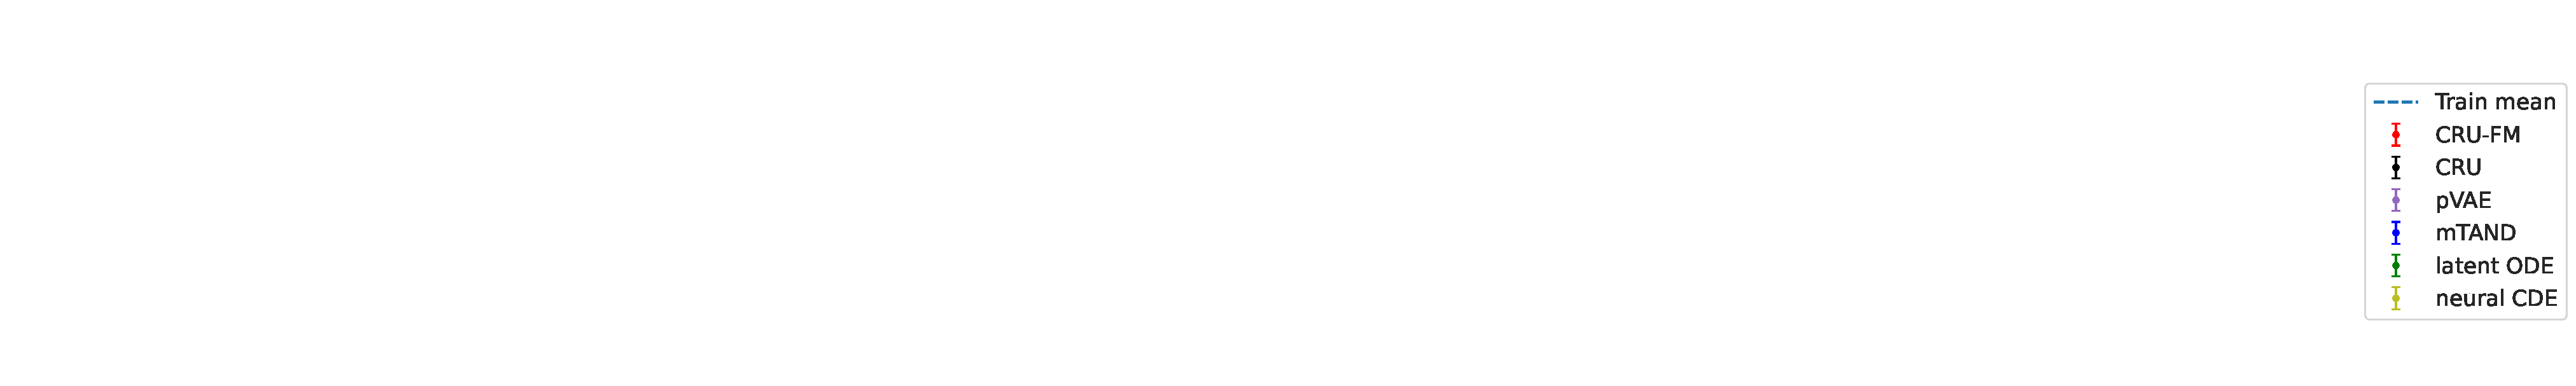
\includegraphics[height=3.5cm]{content/chapters/irregular_time_series_data_driven_missingness/figures/legend.pdf}}
    \\~\\
        \rotatebox{90}{\hspace{4em} Physionet} 
        & 
        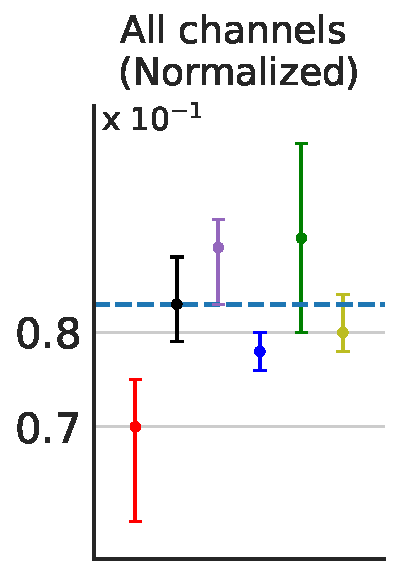
\includegraphics[height=5.2cm]{content/chapters/irregular_time_series_data_driven_missingness/figures/physionet_evaluation_summary.pdf} 
        &
        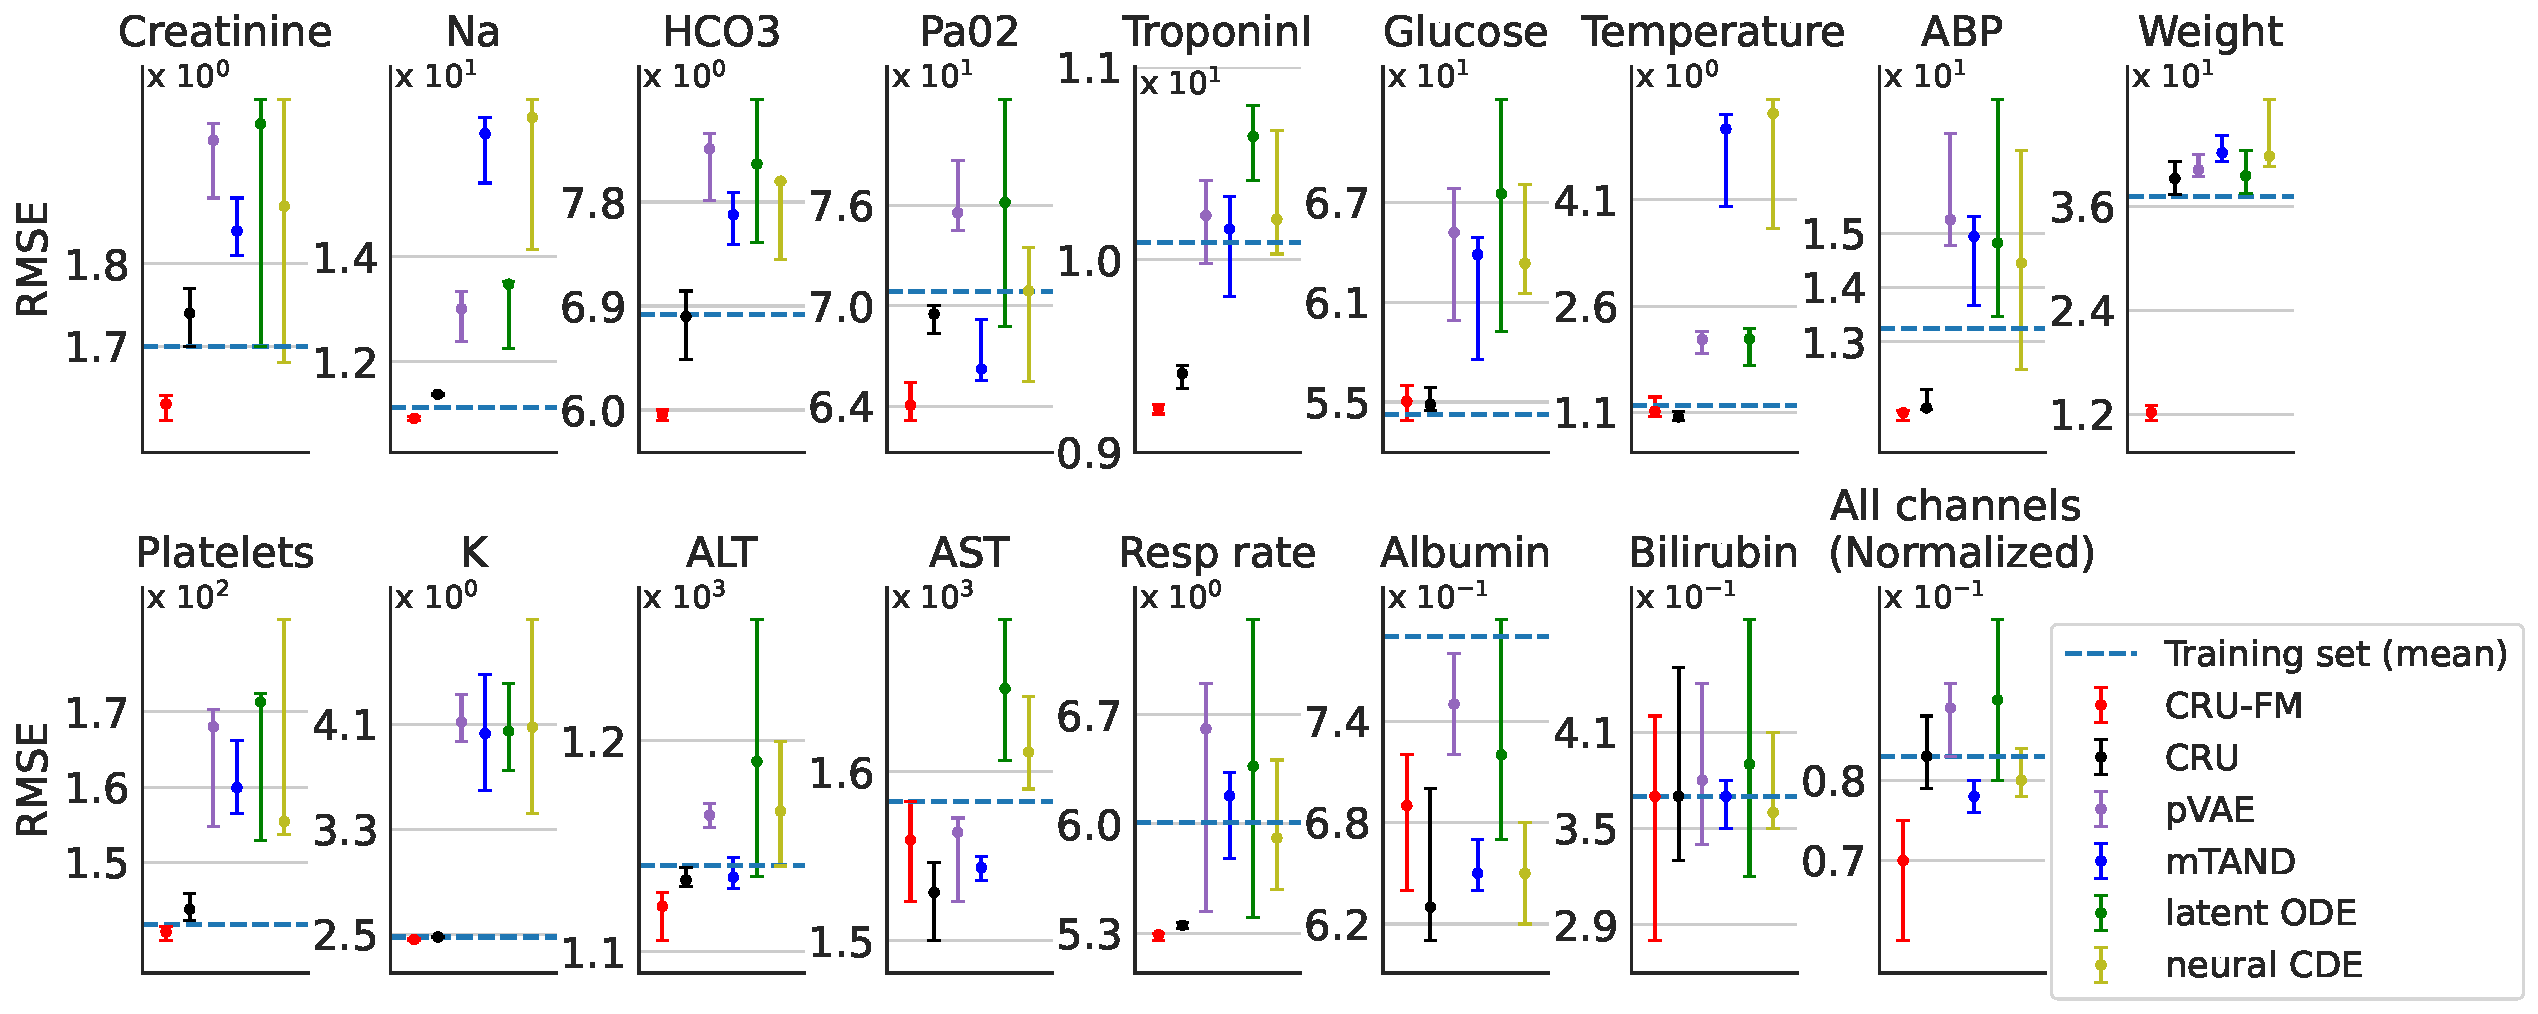
\includegraphics[trim={0 0 590 0},clip,height=5.2cm]{content/chapters/irregular_time_series_data_driven_missingness/figures/physionet_evaluation.pdf}
    \\~\\
        \rotatebox{90}{\hspace{4em} eICU}
        &
        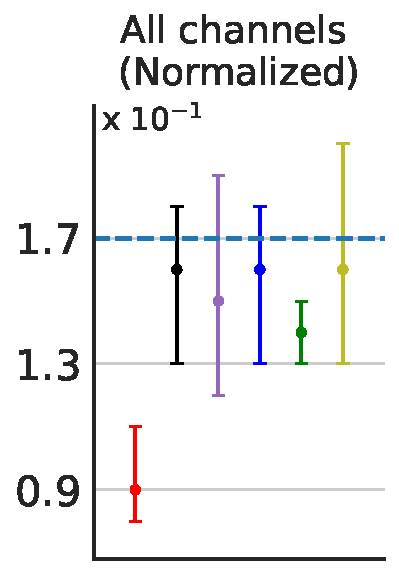
\includegraphics[height=5.2cm]{content/chapters/irregular_time_series_data_driven_missingness/figures/eicu_evaluation_summary.pdf} 
        &
        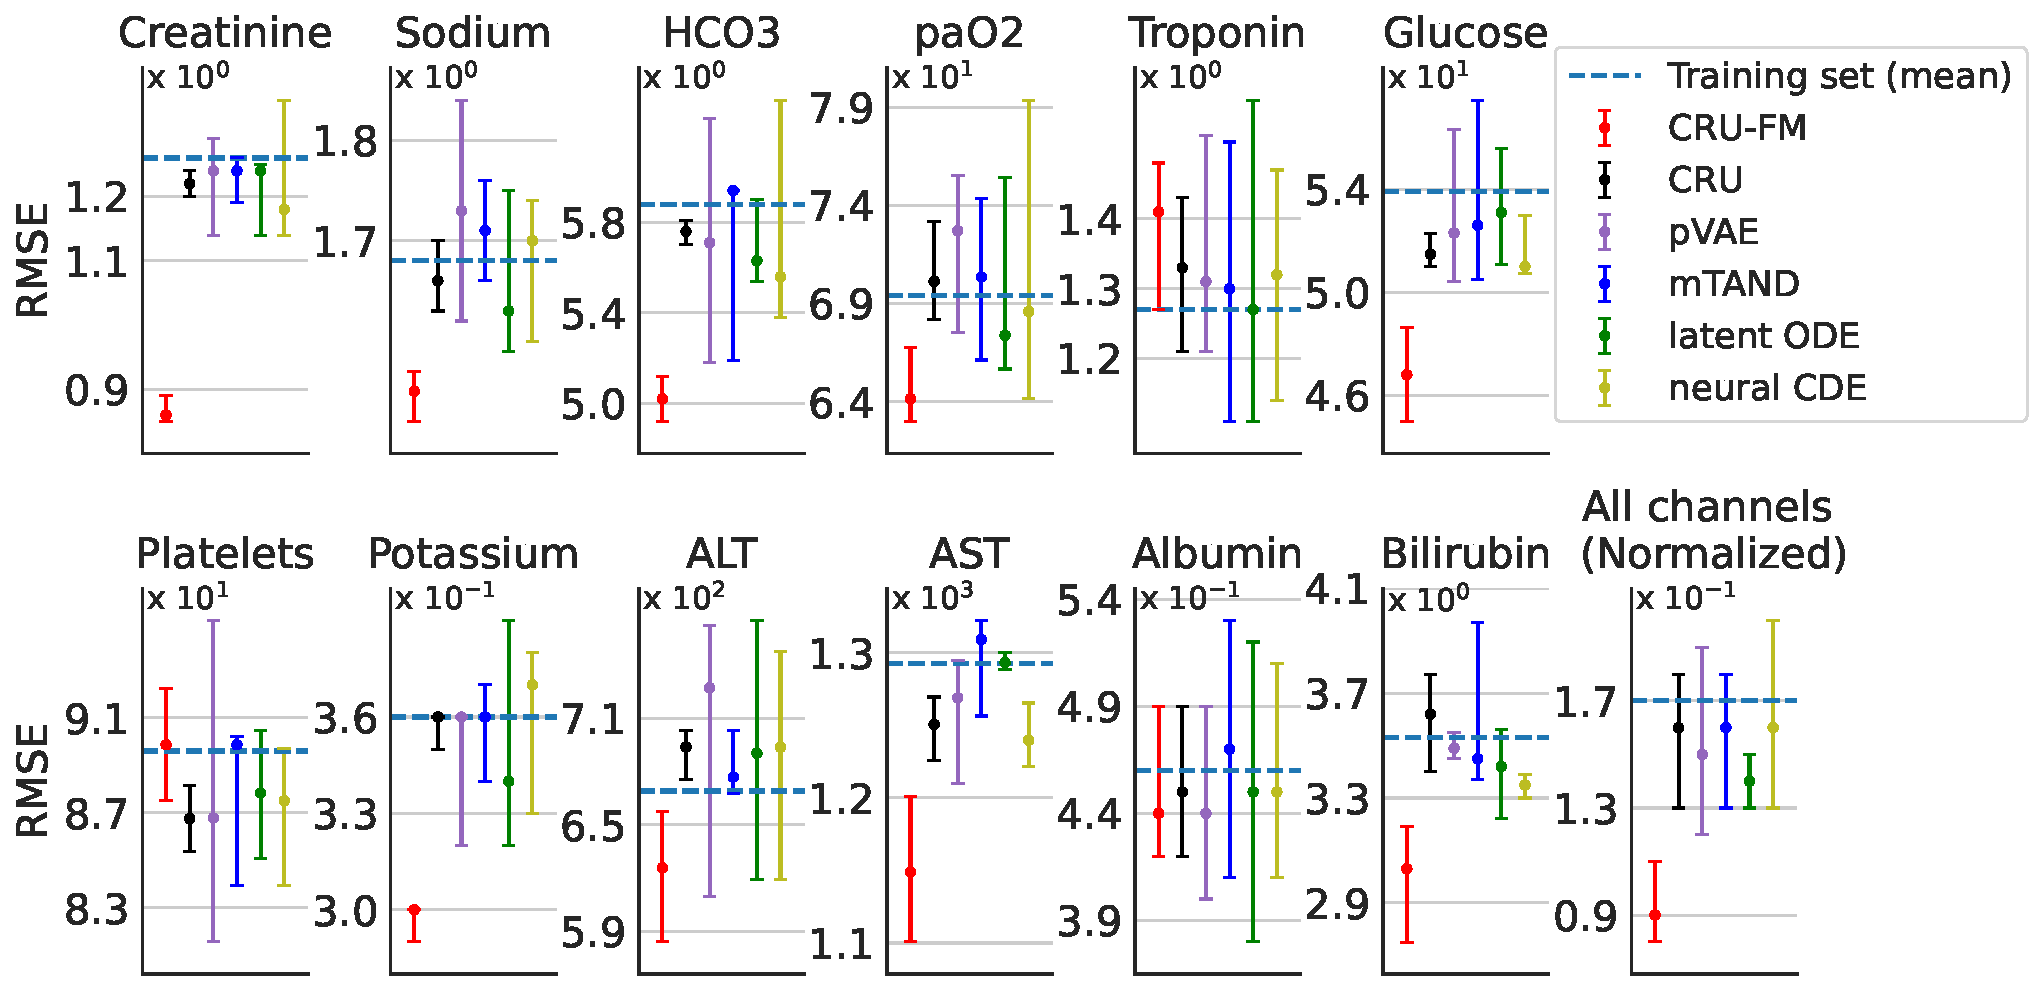
\includegraphics[trim={0 0 355 0},clip,height=5.2cm]{content/chapters/irregular_time_series_data_driven_missingness/figures/eicu_evaluation.pdf}
    \end{tabular}
    \caption[Comparison of extrapolating measurements with our CRU-FM v/s 5 competitor methods on 3 EHR datasets]{Comparison of our CRU-FM with 5 competitor methods, in terms of extrapolation error (RMSE, lower is better) on MIMIC-IV, Physionet, and eICU test sets. For each test patient-stay, the first 24 hours of data are provided as input, and methods must extrapolate the next 6-24 hours of available measurements. Confidence intervals show the 5th and 95th percentiles of the mean RMSE across 100 bootstrapped samples of the test set. 
    Our CRU-FM clearly outperforms competitors in overall error across all channels (left column). Per-channel error comparisons (right columns) for select channels also show clear wins in a majority of cases (CRU-FM's confidence interval is lower and does not overlap with others). Expanded per-channel results for all datasets in App. Fig. \ref{fig:all_channels_evaluation_extended}  
    }%endcaption
    \label{fig:real_data_evaluation}
\end{figure}

\textbf{eICU setup.} 
 Out of the over 200,000 ICU-stays in the multi-hospital eICU dataset \citep{johnson2020mimic}, we select 
 all patient stays that last at least 30 hours.
For each stay, we track 12 labs (see Tab.~\ref{tab:eicu_features}).
We exclude channels like respiratory rate, temperature and arterial blood pressure as these measurements are collected more regularly.
Our train/valid/test splits have 63555/15889/19862 patient-stays. 
\begin{table}[ht]
    \centering
    \begin{tabular}{|c|c|c|c|} \hline 
         Feature&  Min&  Max& Observation rate per hour  (averaged over first 48 hours)\\ \hline 
         TroponinT&  0.01&  11.8& 0.002\\ \hline 
         Bilirubin&  0.01&  12.8& 0.002\\ \hline 
         ALT&  6.00&  2565.8& 0.017\\ \hline 
         AST&  8.00&  3773.2& 0.017\\ \hline 
         Albumin&  1.30&  4.30& 0.019\\ \hline 
         HCO3&  9.00&  44.09& 0.022\\ \hline 
         PaO2&  37.0&  447.0& 0.023\\ \hline 
         Platelets&  27.0&  504.0& 0.047\\ \hline 
         Creatinine&  0.36&  9.07& 0.054\\ \hline 
 Glucose& 64.0& 442.0&0.056\\ \hline 
 Sodium& 119.0& 156.0&0.059\\ \hline 
 Potassium& 2.7& 6.2&0.065\\\hline
    \end{tabular}
    \caption{List of features for eICU}
    \label{tab:eicu_features}
\end{table}


\textbf{Measuring uncertainty.}
For each method on each dataset, we record its RMSE when extrapolating on the test set. To construct uncertainty intervals, we follow \citet{raschka2018model} and perform bootstrap sampling (with replacement) from the entire test set 100 times. For each of the 100 sets, we evaluate the RMSE and report the median, 5th and 95th percentiles.
%in  Fig.~\ref{fig:real_data_evaluation}. 

\paragraph{Results: Overall extrapolation error.}
For each dataset in Fig.~\ref{fig:real_data_evaluation}, a panel labeled ``All channels (normalized)'' reports  overall performance across all examined vitals and labs (even those not depicted in other panels).
This requires normalizing actual and predicted values from each channel to a 0-1 scale using the min and max estimates from the training set, then computing the average RMSE.
Across all 3 datasets, our CRU-FM consistently scores better than any competitor on this overall error.



In addition to our CRU-FM and the 5 competitor methods for irregular time series, we include a simpler baseline that always predicts the mean of the training set values for each channel. 
This baseline predicts the same future for all patients and thus is not clinically useful.
Our all-channel results suggest surprisingly that some competitor methods do not always surpass even this baseline.
Previous studies~\citep{shukla2021multitime, rubanova2019latent} have overlooked such simple baselines, focusing solely on comparing neural network methods. We include it to demonstrate that existing complex models frequently do not outperform such basic approaches, indicating a key need for improvement in the present landscape of irregular time series methods we hope our method fills.

\paragraph{Results: Individual feature extrapolation.}
Other panels in Fig.~\ref{fig:real_data_evaluation} each show RMSE for a specific vital sign or lab  common across datasets. We report such RMSE values in the corresponding variable's original units (un-normalized) to help contextualize any gains shown on a physiological scale more familiar to clinicians.
Not all vitals or labs are shown here due to space constraints; see Figure \ref{fig:all_channels_evaluation_extended} for results on an extended list of channels beyond those in Figure \ref{fig:real_data_evaluation}.
%on the overlapping set of 11 labs common across all 3 datasets. 
Across the extended channels shown in Fig.~\ref{fig:all_channels_evaluation_extended}, we find the CRU-FM model achieves the clearly lowest RMSE (the red interval lies below the interval for any other method by visual inspection) in 11/16 features from physionet, 8/16 from MIMIC-IV, and 7/12 from eICU. In several other cases, the CRU-FM is essentially ``tied'' with one or more other methods. These per-channel results, together with the CRU-FM's overall win, suggest the value of our approach.

CRU-FM does not seem clearly superior to alternatives on channels such as respiratory rate that are collected more frequently, perhaps because they are less likely to be missing and there is less need for a data-dependent mechanism. However, for lab measurements such as Creatinine, Troponin, ALT that are measured less frequently, the CRU-FM outperforms other baselines in at least 2/3 datasets. 

\paragraph{Qualitative visuals of extrapolations.} We  illustrate examples of extrapolation on 3 randomly picked patient stays in Figure \ref{fig:example_extrapolation_eICU}.
These plots illustrate improved extrapolations (and interpolations) for our CRU-FM compared to the CRU. 

\begin{figure}[htbp]
    \centering 
    \begin{tabular}{cc}
        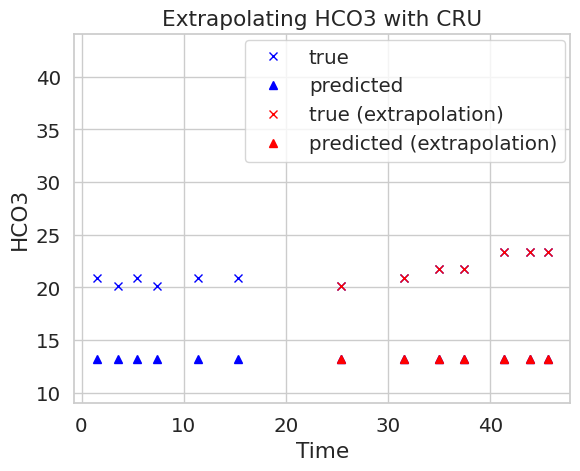
\includegraphics[width=0.45\linewidth]{content/chapters/irregular_time_series_data_driven_missingness/figures/true_vs_predicted_HCO3_cru.png} & 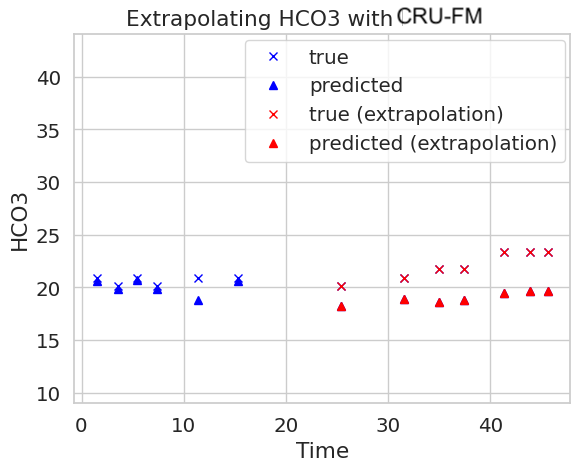
\includegraphics[width=0.45\linewidth]{content/chapters/irregular_time_series_data_driven_missingness/figures/true_vs_predicted_HCO3_mnar_cru.png} \\
        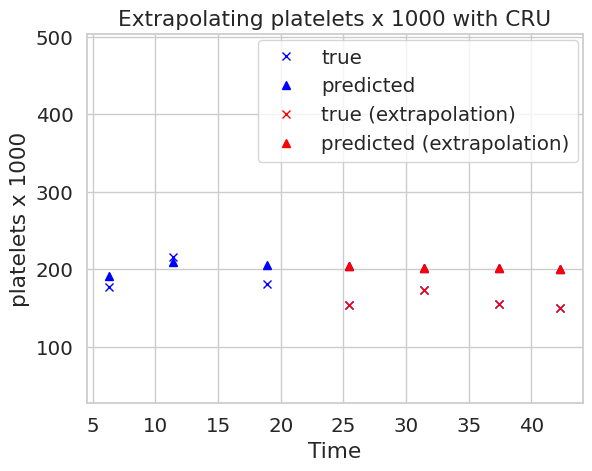
\includegraphics[width=0.45\linewidth]{content/chapters/irregular_time_series_data_driven_missingness/figures/true_vs_predicted_platelets_cru.png} & 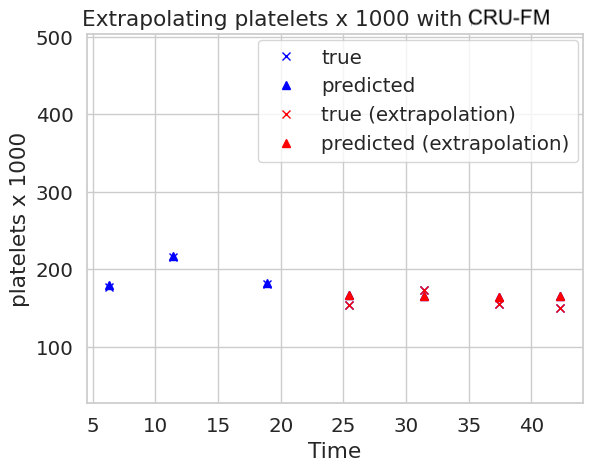
\includegraphics[width=0.45\linewidth]{content/chapters/irregular_time_series_data_driven_missingness/figures/true_vs_predicted_platelets_mnar_cru.png} \\
        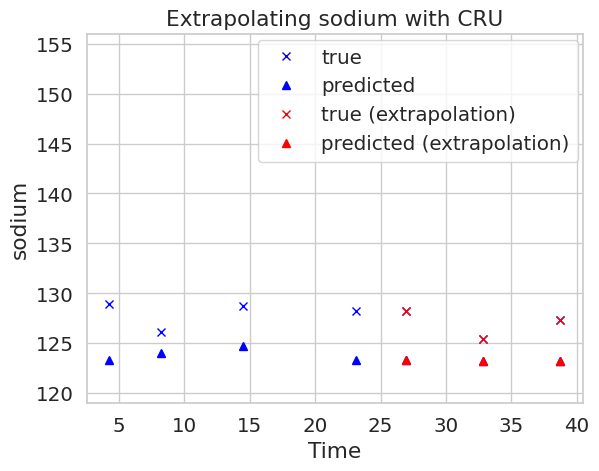
\includegraphics[width=0.45\linewidth]{content/chapters/irregular_time_series_data_driven_missingness/figures/true_vs_predicted_sodium_cru.png} & 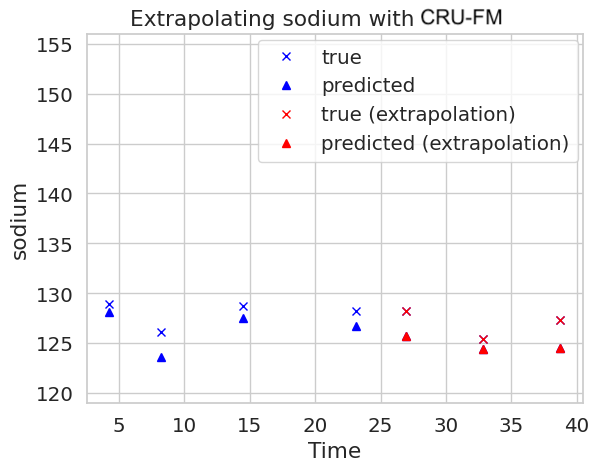
\includegraphics[width=0.45\linewidth]{content/chapters/irregular_time_series_data_driven_missingness/figures/true_vs_predicted_sodium_mnar_cru.png} \\
    \end{tabular}
    \caption{Illustrative examples of predicted trajectories from the eICU dataset, demonstrating that our CRU-FM outperforms the CRU in both extrapolation and interpolation of sequences.} 
    \label{fig:example_extrapolation_eICU} 
\end{figure}

\paragraph{Alternative method: CRU for concatenation of features and missingness mask.}
To confirm that improvements in our model stem from its ability to learn the mechanism of missing data, we introduced another baseline in which the missingness indicator mask $s_t$ is incorporated into the CRU as extra input feature channels. 
Below, we report results comparing our CRU-FM with the vanilla CRU with both features and missingness masks as inputs.

\begin{table}[ht]
\centering
\label{tab:cru_fm_vs_cru_w_mask}
\begin{tabular}{lcc}
\toprule
Lab Measurement & CRU-FM (test RMSE) & CRU w/ missing mask (test RMSE) \\ 
\midrule
creatinine & \textbf{0.86 (0.85, 0.89) }& 1.25 (1.22, 1.29) \\
potassium & \textbf{0.30 (0.29, 0.30)} & 0.38 (0.36, 0.41) \\
Sodium & \textbf{1.55 (1.52, 1.57)} & 1.77 (1.70, 1.82) \\
Platelets x 1000 & \textbf{89.86 (87.53, 92.22)} & 91.75 (89.66, 93.29) \\
Glucose & \textbf{46.81 (45.00, 48.63)} & 53.66 (53.10, 55.15) \\
HCO3 & \textbf{5.02 (4.92, 5.12)} & 6.01 (5.88, 6.18) \\
paO2 & \textbf{64.16 (63.00, 66.78)} & 73.22 (69.04, 77.21) \\
albumin & \textbf{0.44 (0.42, 0.49)} & 0.51 (0.48, 0.53) \\
ALT & \textbf{625.80 (584.00, 657.63)} & 696.52 (688.74, 705.81) \\
AST & \textbf{1148.96 (1100.80, 1200.86)} & 1248.19 (1236.01, 1271.91) \\
Bilirubin & \textbf{3.03 (2.75, 3.19)} & 3.80 (3.65, 3.84) \\
Troponin & 1.41 (1.27, 1.48) & \textbf{1.31 (1.20, 1.44) }\\
\bottomrule
\end{tabular}
\caption[Test RMSE of CRU (w/missing mask as input) and our CRU-FM on eICU dataset]{Comparing Test RMSE of CRU (w/missing mask as input) and our CRU-FM on the eICU dataset. In 11 out of 12 channels, our proposed method does better in terms of test RMSE.}
\end{table}


\paragraph{Predicting future missingness of a channel.} 
We additionally conduct  an experiment on the eICU and MIMIC-IV datasets assessing how jointly modeling features and missingness can predict future missingness of one particular channel (creatinine), chosen because it is infrequently observed and as a blood draw is likely to depend on data-driven decision-making. 
 
For each sequence in the test set :
	In interval $24h<t''<24h+w$ (window length) :
		Predict $s_{t'', creatinine} \in \{0, 1\}$ (predict if a measurement will be observed)

We trained a linear classifier (L2-penalized logistic regression) for 4 distinct scenarios that vary the input features fed into the classifier listed below:
\begin{itemize}
\item MCAR: input feature is just p, where p  is the patient-specific rate of observing a creatinine measurement in the first 24 hours (before the prediction interval)

\item Last observation only (MAR simple): classify $s_{t'', creatinine}|X_{obs},t'$, where $t'\in \mathbb{R}^D$ and $X_{obs}$, $t'\in \mathbb{R}^D$ is the last observed time point and measurement for each channel before 24 hours.

\item Modeling features only (MAR CRU) : classify $s_{t'', creatinine}|\mu_{t'_{24}}$ , where $\mu_{t'_{24}}$ refers to the representation vector  at time t=24 produced by the CRU model.

\item Modeling features + missingness (MAR CRU-FM) : classify $s_{t''}, creatinine|\mu_{t_{24}}$, where $\mu_{t_{24}}$ refers to the representation vector  at time t=24 produced by our model
\end{itemize}

Below for each model and possible window length, we report AUROC intervals computed from 100 bootstrapped samples on test set. % for various window lengths.

\begin{table}[ht]
\centering
\label{tab:missingness_classification_experiement}
\resizebox{.95\textwidth}{!}{
\begin{tabular}{llcccc}
\toprule
Dataset & Window Len. & MCAR & MAR Simple & MAR CRU & MAR CRU-FM \\ 
\midrule
\multirow{3}{*}{eICU} & 2 hours & 0.61 (0.57, 0.62) & 0.61 (0.59, 0.61) & 0.64 (0.63, 0.66) & \textbf{0.70 (0.69, 0.72)} \\
                      & 4 hours & 0.62 (0.58, 0.63) & 0.62 (0.60, 0.62) & 0.65 (0.63, 0.67) & \textbf{0.72 (0.70, 0.75)} \\
                      & 6 hours & 0.64 (0.60, 0.64) & 0.64 (0.62, 0.65) & 0.68 (0.66, 0.69) & \textbf{0.73 (0.71, 0.74)} \\
\hline
\multirow{3}{*}{MIMIC-IV} & 2 hours & 0.64 (0.63, 0.66) & 0.65 (0.63, 0.66) & 0.67 (0.66, 0.69) & \textbf{0.72 (0.69, 0.73)} \\
                          & 4 hours & 0.67 (0.64, 0.69) & 0.67 (0.66, 0.67) & 0.69 (0.68, 0.70) & \textbf{0.74 (0.70, 0.74)} \\
                          & 6 hours & 0.70 (0.69, 0.72) & 0.68 (0.66, 0.69) & 0.69 (0.68, 0.71) & \textbf{0.75 (0.72, 0.76)} \\
\bottomrule
\end{tabular}
}%endresizebox
\caption[Performance comparison for predicting future missingness of a channel]{The table presented above clearly illustrates the superiority of our model's approach—utilizing our CRU-FM’s representation vector for predicting the likelihood of a measurement occurring within a specified window, yields better AUROC compared to the alternative methods of relying solely on past observations or the simplistic strategy of utilizing a patient-specific observation rate (MCAR). Additionally, the improvement in AUROC as the window length increases can be attributed to the increase in ground truth positives.}
\end{table}

\paragraph{Extrapolation performance on extended list of channels}
In figure \ref{fig:all_channels_evaluation_extended}, we report the extrapolation performance on an extended list of channels beyond those reported in figure \ref{fig:real_data_evaluation}.
\begin{table*}[!tp]
    \centering
    \begin{tabular}{|l |c|}
        \hline        \rotatebox{90}{\hspace{3em}MIMIC-IV} 
        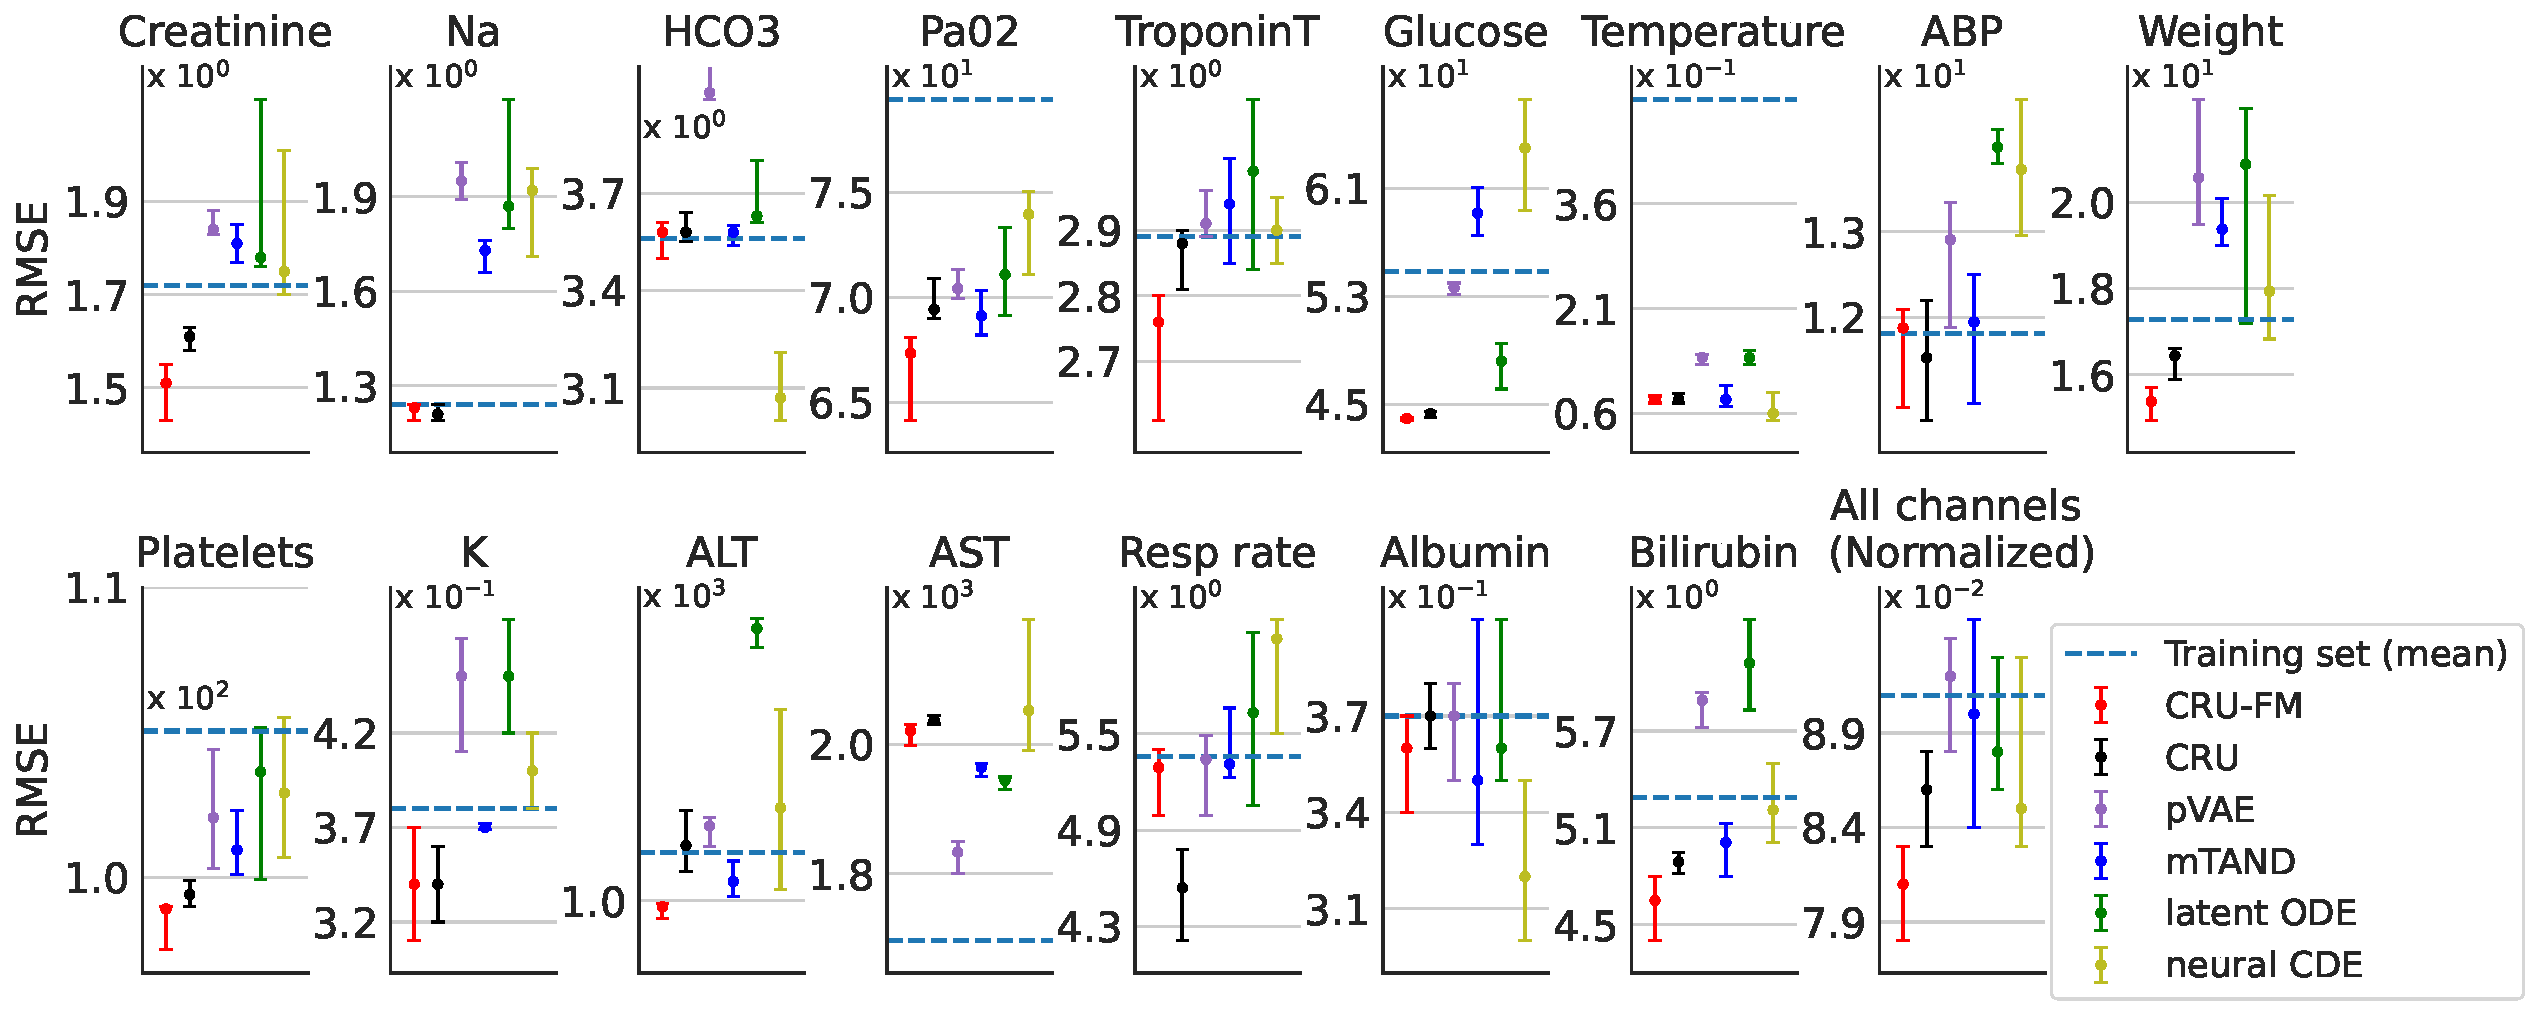
\includegraphics[width=0.95\textwidth]{content/chapters/irregular_time_series_data_driven_missingness/figures/mimic_evaluation.pdf} 
        \\~\\
        \hline
        \rotatebox{90}{\hspace{4em} Physionet} 
        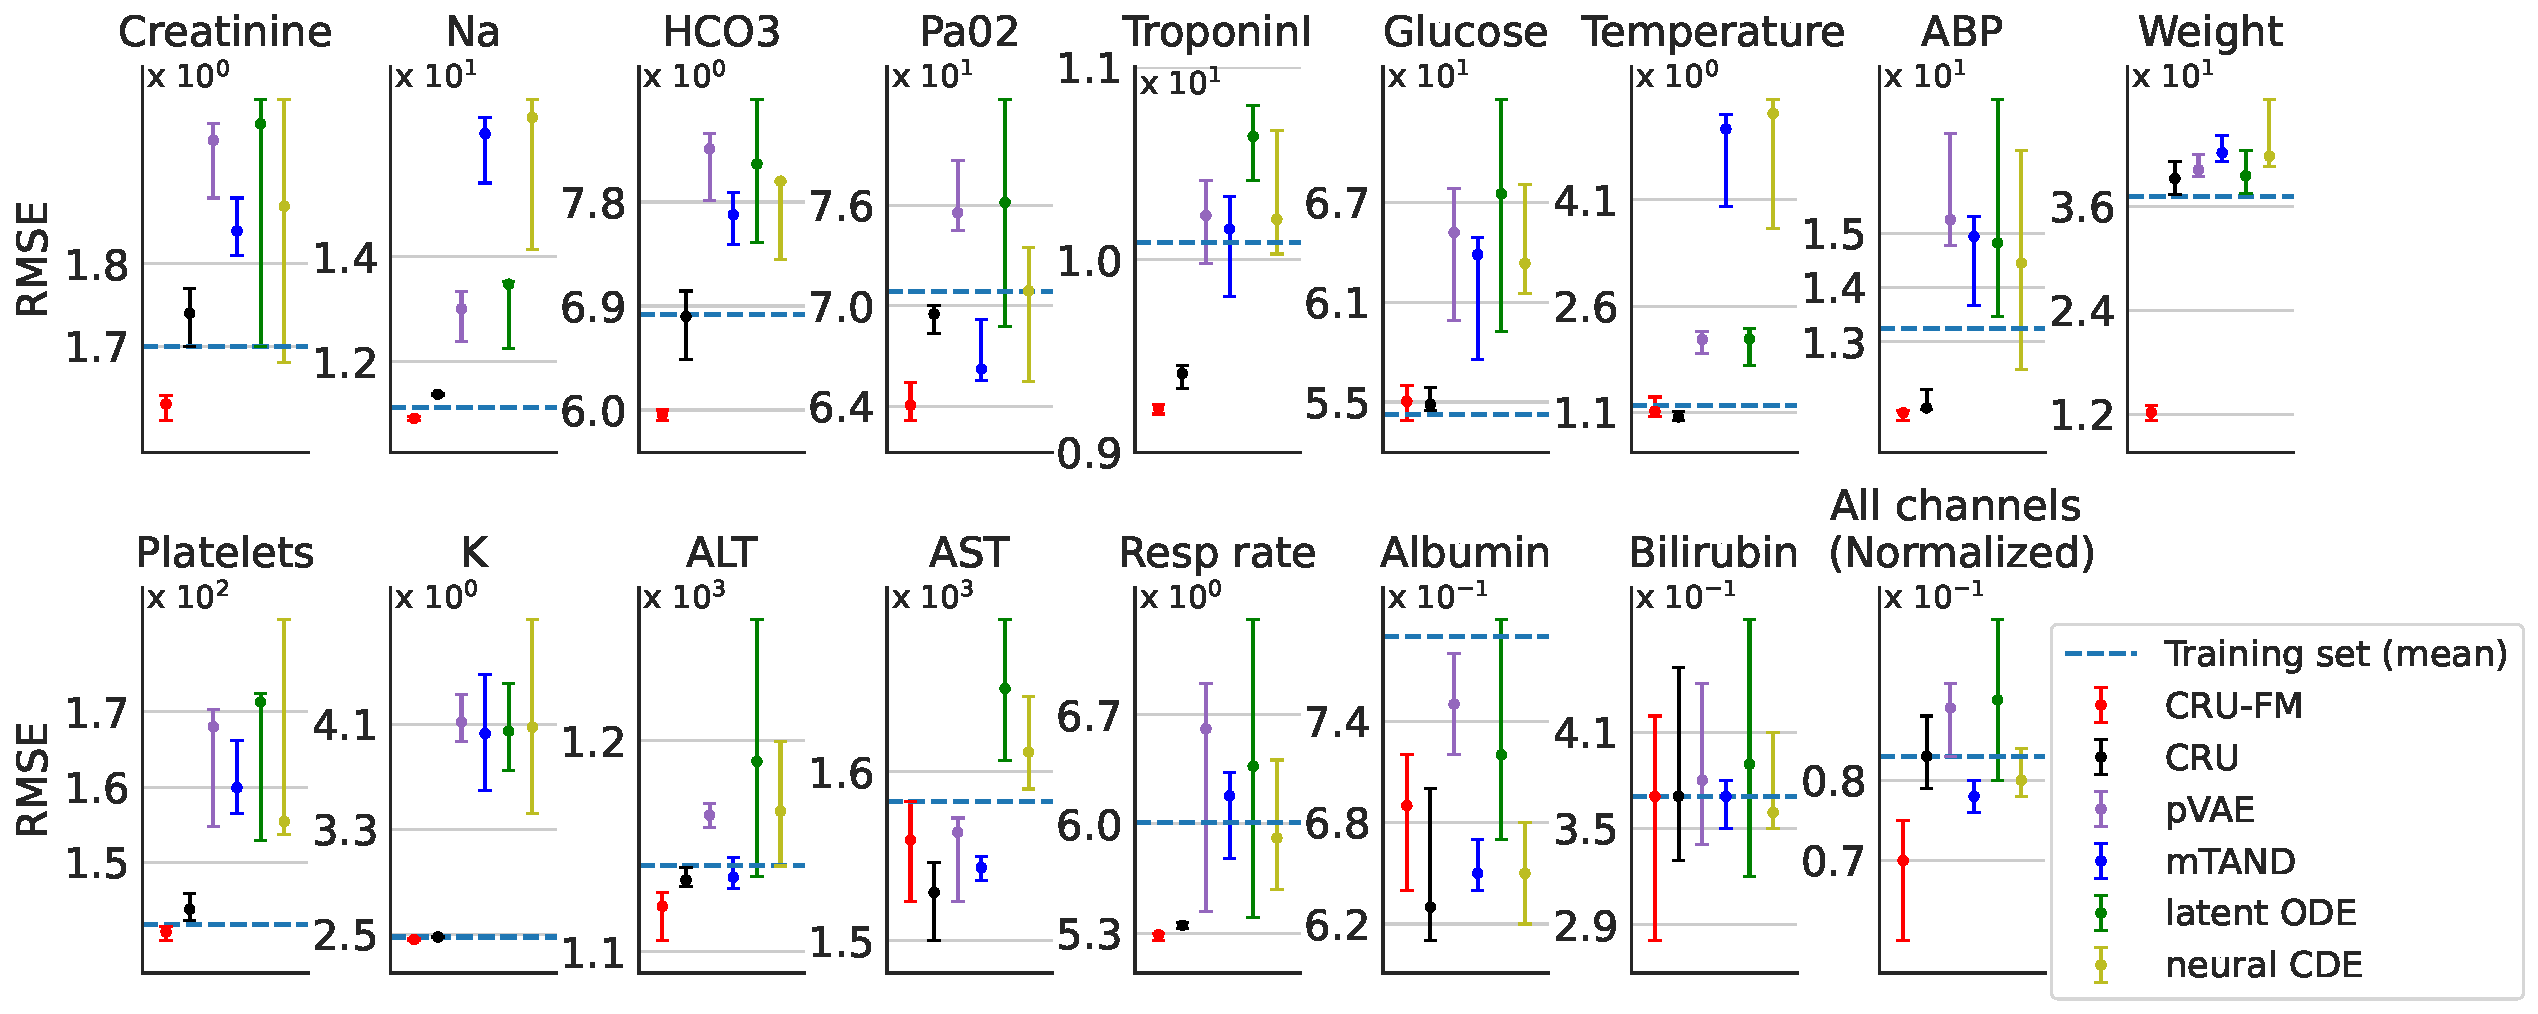
\includegraphics[width=0.95\textwidth]{content/chapters/irregular_time_series_data_driven_missingness/figures/physionet_evaluation.pdf} 
        \\~\\
        \hline
        \rotatebox{90}{\hspace{4em} eICU}
        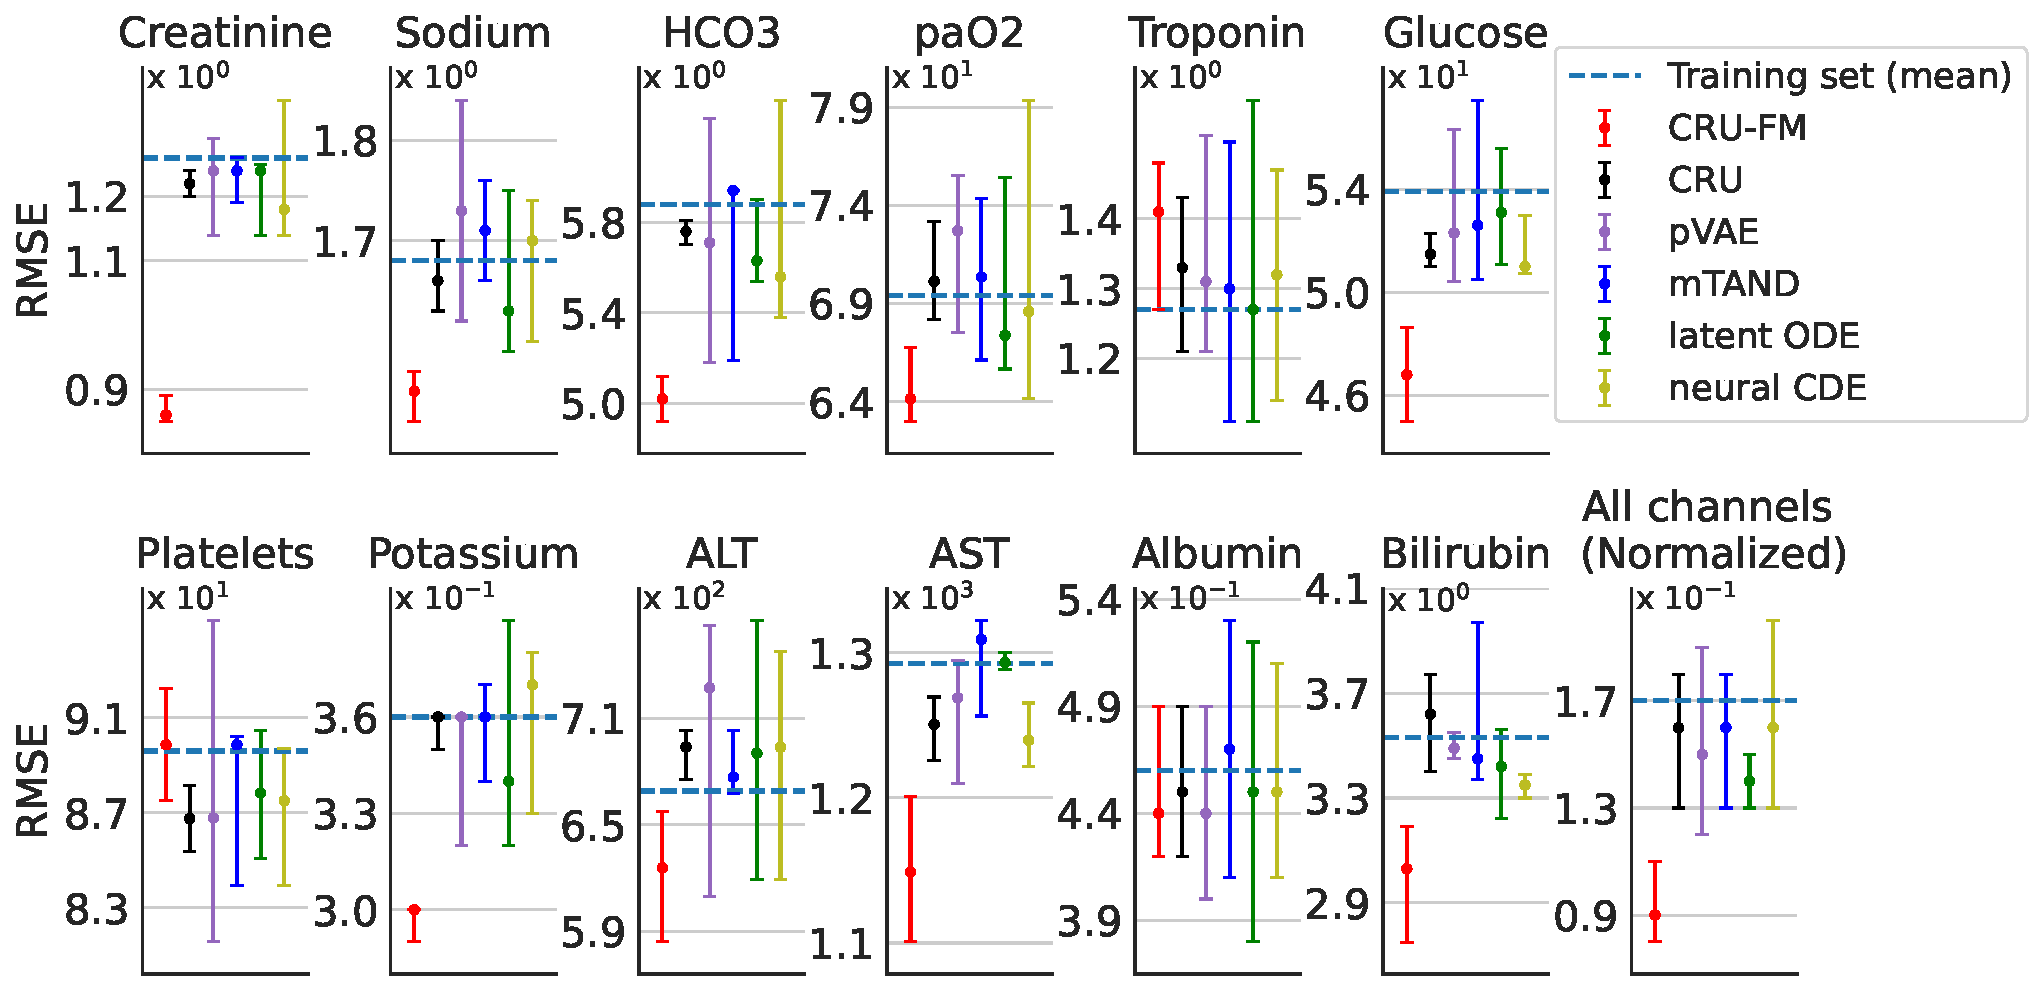
\includegraphics[width=0.95\textwidth]{content/chapters/irregular_time_series_data_driven_missingness/figures/eicu_evaluation.pdf}\\
        \hline
    \end{tabular}
    \caption[Extrapolation performance on extended list of channels on 3 EHR datasets comparing 5 baselines with our CRU-FM]{RMSE comparison of our CRU-FM with 5 baselines after training on the first 24 hours of data and extrapolating the next 24 hours of measurements on MIMIC-4, Physionet, and eICU. Confidence intervals represent the 5th and 95th percentiles from 100 bootstrapped samples from the test set. Our CRU-FM outperforms baselines in 8/16 channels in MIMIC-4, 11/16 channels on Physionet and 7/12 channels in eICU (RMSE confidence intervals are lower and do not overlap with baselines). The training set mean baseline is added to uncover a gap in existing studies \citep{shukla2021multitime, rubanova2019latent}, which overlooked a simple yet effective benchmark that, while showing decent RMSE performance, falls short in complex clinical decision-making settings.}
    \label{fig:all_channels_evaluation_extended}
\end{table*}

\section{Conclusion}
We present a novel approach to modeling irregular time series data that can learn mechanisms for \emph{data-dependent missingness}. On all 3 large EHR datasets studied, our improved handling of missingness yields noticeably lower overall extrapolation error than several recent competitors.
While joint modeling of missingness indicators and observed features could be accomplished with many model architectures, by building upon \citet{schirmer2022modeling}'s  CRU backbone our implementation benefits from efficient computations and avoids the need for expensive ODE/SDE solvers.
Future work could investigate the even more flexible missing-not-at-random (MNAR) setting for irregular time series; 
though empirically every MNAR model has a MAR counterpart with equal fit 
\citep{molenbergsCounterpart2008} and thus the choice of MNAR requires belief in the underlying model assumptions not easily confirmed via empirical error analysis alone. More research is also necessary to ensure that our model's superior extrapolation capabilities translate effectively into enhanced clinical understanding and improved patient care. Additionally, while our comparisons are currently limited to other irregular time series models, examining how our approach stacks up against different types of models could provide broader insights. Lastly, identifying which specific vitals or lab results our methods most effectively predict remains an open question.

\chapter{Conclusion and Outlook}
% Summarize main question
This thesis thesis has explored the question of how to evaluate, train, and benchmark machine learning models for decision making problems. \

% Summarize BPR
In Chapter 3, we demonstrated how decision-aware model selection can lead to better public health outcomes.
We also introduced a new evaluation metric called Best Possible Reach which quantifies the decision quality of Top $K$ allocation problems.

% Summarize DAML
This work was extended in Chapter 4 where we demonstrate how a model can be \emph{trained} to maximize both decision quality and probabalistic maximum likelihood, in addition to answer the question of \emph{how to rank} locations based on predicted scores. \
The proposed Decision-Aware Maximum Likelihood method was compared to a small number of other decision aware methods, and found to be superior on the given tasks. \
We also explored problems beyond public health, including a wildlife conservation task.

% Summarize benchmarking
In Chapter 5 we turned our attention to understand why some decision-aware learning methods perform better than others, and to provide practical guidance for practitioners looking to implement these methods. \
Here we decomposed the analysis of decision-aware methods into two components: what solutions does the method prefer, and which solutions is the method capable of learning via gradient descent. \
We also found that many tasks used in common decision-aware benchmarks do not actually benefit from decision-aware methods, and propose several open-source alternatives. 

% Summarize thesis and suggest future benchmarking working
Taken together, these contributions provide end-to-end guidance for the training and evaluation of decision-aware machine learning techniques.
However, crucial open questions remain. Although we have demonstrated the importance of more careful benchmarking comparisons between methods, we still lack an analytical understanding of when decision-aware learning is beneficial, and how this depends on the structure of the downstream optimization problem and the role predictions play in determining the final decision. \
Future work should therefore develop new benchmark tasks that more clearly expose the conditions under which decision-aware learning offers advantages over decision-unaware two-stage approaches. \
Aditionally, new training methods are needed that make more principled use of prediction error within decision-aware learning as suggested in Chapter \ref{chap:daml}. \
Rather than discarding predictive accuracy as irrelevant, these methods should identify which errors are decision-critical and allocate learning effort accordingly, avoiding overemphasis on errors that are either too easy to correct or unlikely to affect the downstream decision. \

% suggest DTR, patient intervention, and inference
Beyond the largely social-science focused problems considered in this thesis, decision-aware methods have widespread applications in many domains. \
One particularly exciting domain is that of machine learning training and inference itself. \
In the twilight of Moore's Law, the rise of expensive foundation model inference has made computational efficiency more important than ever. \
Recent work has shown that by simply sampling more model outputs at test time, performance (as measured by at least one sample getting the correct response) can improve log-linearly with compute \citep{brownLargeLanguageMonkeys2024}.\
This has trasformed the simple act of using a model to output predictions into a budgeting problem. \
How we spend resources at test-time is a meaninful axis of model improvement: \cite{muennighoffS1SimpleTesttime2025a} showed consistent improvement over several-orders of magnitude, taking models from 0 to 60\% accuracy on challenging math datasets, and outperforming pretrined models with many more parameters. \
Here decision-aware methods can help answer the question of how to best spend fixed computational budgets to achieve optimal results from model inference. \
Furthermore, if model inference is now a decision task, should we be training all models in a budget conscious, decision aware way? \
We hope that the methods and findings of this thesis help to explore these questions in future work.
%%%%%%%%%%%%%%%%%%%%%%%%%%%%%%%%%%%%%%%%%%%%%%%%%
% bibliography
%%%%%%%%%%%%%%%%%%%%%%%%%%%%%%%%%%%%%%%%%%%%%%%%%

\bibliographystyle{plainnat}
{
\singlespacing
% \newpage
\phantomsection
\addcontentsline{toc}{chapter}{Bibliography}
% % The following assumes your references are in .bib format.  
\bibliography{refs/thesisbib}
}

\end{document} 